\باب{گھومتے مشین کے بنیادی اصول}
%proof read entire chapter
اس باب میں مختلف گھومتے مشینوں کے بنیادی اصولوں پر غور کیا جائے گا۔ظاہری طور پر مختلف مشین ایک ہی قسم کے اصولوں پر کام کرتے ہیں جنہیں اس باب میں اکٹھا کیا گیا ہے۔

\حصہ{قانون فیراڈے}
\اصطلاح{قانون فیراڈے}\فرہنگ{فیراڈے!قانون}\حاشیہب{Faraday's law}\فرہنگ{Faraday's law} کے تحت جب بھی کسی لچھے کا ارتباط بہاو  \عددیء{\lambda} وقت کے ساتھ تبدیل ہو، اس لچھے میں برقی دباو پیدا ہو گا:
\begin{align}
e=\frac{\partial \lambda}{\partial t}=N \frac{\partial \phi}{\partial t}
\end{align}
چونکہ ہمیں برقی دباو کی قیمت نا کہ اس کے \عددیء{\mp}  سے دلچسپی ہے لہٰذا اس مساوات میں منفی کی علامت کو نظر انداز کیا گیا ہے۔

گھومتے مشین میں ارتباط بہاو کی تبدیلی مختلف طریقوں سے پیدا کی جا سکتی ہے۔مثلاً  لچھے کو ساکن مقناطیسی بہاو میں گھما کر یا  ساکن لچھے میں مقناطیس گھما کر، وغیرہ وغیرہ۔

ان برقی مشینوں میں لچھے مقناطیسی قالب\فرہنگ{قالب}\حاشیہب{magnetic core}\فرہنگ{core}  پر لپیٹے جاتے ہیں۔ اس طرح کم سے کم مقناطیسی دباو سے زیادہ سے زیادہ مقناطیسی بہاو حاصل کیا جاتا ہے اور لچھوں کے مابین مشترکہ مقناطیسی بہاو بڑھایا جاتا ہے۔ مزید قالب کی شکل تبدیل کر کہ مقناطیسی بہاو کو ضرورت کے مقام پر پہنچایا جاتا ہے۔

ان مشینوں کے قالب میں مقناطیسی بہاو وقت کے ساتھ تبدیل ہوتا ہے لہٰذا قالب میں بھنور نما برقی رو\فرہنگ{بھنور نما برقی رو}\فرہنگ{برقی رو!بھنور نما}\حاشیہب{eddy currents}\فرہنگ{eddy currents} پیدا ہوتا ہے۔ان بھنور نما برقی رو کو کم سے کم کرنے کی خاطر  باریک لوہے کی پتری\فرہنگ{پتری}\حاشیہب{laminations}\فرہنگ{laminations} تہہ در تہہ رکھ قالب بنایا جاتا ہے ۔  آپ کو یاد ہو گا، ٹرانسفارمر کا قالب بھی اسی طرح بنایا جاتا ہے۔

\حصہ{معاصر مشین}
شکل \حوالہ{شکل_گھومتے_مشین_دو_قطب_ایک_دور_معاصر_بنیادی_شکل}  میں \اصطلاح{معاصر} برقی جنریٹر کا ایک بنیادی شکل دکھایا گیا ہے۔ اس کے قالب میں ایک مقناطیس ہے جو کہ گھوم سکتا ہے۔ مقناطیس کا مقام اس کے میکانی زاویہ \عددیء{\theta_m} سے بتلائی جاتی ہے۔ افقی لکیر سے گھڑی کے مخالف زاویہ \عددیء{\theta_m} ناپا جاتا ہے۔

یہاں کچھ باتیں وضاحت طلب ہیں۔ اگر مقناطیس ایک مقررہ رفتار سے، فی سیکنڈ \عددیء{n}  مکمل چکر کاٹتا ہو تب ہم کہتے ہیں کہ اس مقناطیس کے گھومنے کا تعدد \عددیء{n}  ہرٹز\حاشیہب{Hertz} ہے۔اسی بات کو یوں بھی بیان کیا جاتا ہے کہ مقناطیس \عددیء{60n} چکر فی منٹ\فرہنگ{چکر فی منٹ}\حاشیہب{rounds per minute, rpm} کی رفتار سے گھوم رہا ہے۔ آپ جانتے ہیں کہ ایک چکر \عددیء{360\degree} زاویہ یا \عددیء{2 \pi} ریڈیئن\حاشیہب{radians}  پر مشتمل ہوتا ہے لہٰذا  گھومنے کی اس رفتار کو \عددیء{2\pi n} ریڈیئن فی سیکنڈ بھی کہہ سکتے ہیں۔ یوں اگر مقناطیس \عددیء{f} ہرٹز کی رفتار سے گھوم رہا ہو تب یہ \عددی{2\pi f} ریڈیئن فی سیکنڈ کی رفتار سے گھومے گا جس کو \عددی{\omega} سے ظاہر کیا جاتا ہے۔
\begin{align}
\omega =2\pi f
\end{align}
اس کتاب میں گھومنے کی رفتار کو عموماً ریڈیئن فی سیکنڈ میں بیان کیا جائے گا۔
\begin{figure}
\centering
%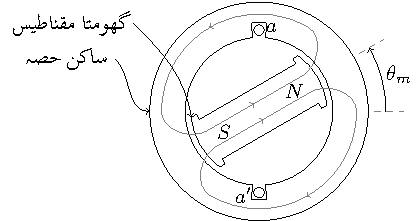
\includegraphics{figRotatingMachPrinciplesTwoPoleSinglePhaseSynchronousMachineBasic}
\begin{tikzpicture}
\stator{2}{90}
\rotor{2}{30}
%FLUX
\begin{scope}[rotate=30]
\pgfmathsetmacro{\delAngle}{30}   %smooth flux entry into stator
\draw[gray] (0,\rT/5)--++(0:0.8*\rR) to [out=0,in=-90+\delAngle] (\delAngle:\sRo-0.2) arc (\delAngle:180-\delAngle:\sRo-0.2)coordinate (leftUpperFlux);
\draw[gray,<-](0,\rT/5)--++(180:0.8*\rR) to [out=180,in=-90-\delAngle] (leftUpperFlux);
\draw[gray,->] (90-1:\sRo-0.2) to [out=180,in=0](90+1:\sRo-0.2);
\draw[gray] (0,-\rT/5)--++(0:0.8*\rR) to [out=0,in=90-\delAngle] (-\delAngle:\sRo-0.2) arc (-\delAngle:-180+\delAngle:\sRo-0.2)coordinate (leftLowerFlux);
\draw[gray,<-](0,-\rT/5)--++(180:0.8*\rR) to [out=180,in=90+\delAngle] (leftLowerFlux);
\draw[gray,->] (-90+1:\sRo-0.2) to [out=180,in=0](-90-1:\sRo-0.2);
\draw node at (0:0.6*\rR){$N$};
\draw node at (180:0.6*\rR){$S$};
\end{scope}
\slotEmptyCircle{90,-90}
\slotName{90/a/right,270/a'/left}
\draw [gray,dashed](0:\sRo+0.1)--++(0:0.5);
\draw [gray,dashed](30:\sRo+0.1)--++(30:0.5);
\draw[->] ([shift={(0:\sRo+0.3)}]0,0) arc (0:30:\sRo+0.3);
\draw node at (30/2:\sRo+0.6){$\theta_m$};
\draw node[left,->] at (160:1.4*\sRo){\RL{ساکن حصہ}};;
\draw[->] (160:1.4*\sRo) to [out=-45,in=180] (180:\sRo);
\draw node[left,->] at (145:1.4*\sRo){\RL{گھومتا مقناطیس}};;
\draw[->] (145:1.4*\sRo) to [out=-45,in=100] (185:\rR);
\end{tikzpicture}
\caption{دو قطب، یک دوری معاصر جنریٹر۔}
\label{شکل_گھومتے_مشین_دو_قطب_ایک_دور_معاصر_بنیادی_شکل}
\end{figure}

شکل \حوالہ{شکل_گھومتے_مشین_دو_قطب_ایک_دور_معاصر_بنیادی_شکل} میں  مشین کے دو مقناطیسی  قطب ہیں، اس لئے اس کو دو قطبی مشین کہتے ہیں۔ ساکن قالب میں، اندر کی جانب دو  شگاف ہیں، جن میں  \عددیء{N} چکر کا لچھا موجود ہے۔ لچھے کو \عددیء{a} اور \عددیء{a'} سے ظاہر کیا گیا ہے۔اس لچھے کی بنا اس مشین کو ایک لچھے کا مشین بھی کہتے ہیں۔ چونکہ یہ لچھا جنریٹر کے ساکن حصہ پر پایا جاتا ہے لہٰذا  یہ لچھا  بھی ساکن  ہو گا جس کی بنا اسے  \اصطلاح{ساکن لچھا}\فرہنگ{ساکن لچھا}\حاشیہب{stator coil}\فرہنگ{stator coil} کہتے ہیں۔

مقناطیس کا مقناطیسی بہاو شمالی قطب\حاشیہب{north pole}  \عددیء{N} سے خارج ہو کر خلائی درز میں سے ہوتا ہوا، باہر گول قالب میں سے گزر کر، دوسرے خلائی درز میں سے ہوتا ہوا، مقناطیس کے جنوبی قطب\حاشیہب{south pole}   \عددیء{S} میں داخل ہو گا۔ اس مقناطیسی بہاو کو  ہلکی سیاہی کے لکیروں سے دکھایا گیا ہے۔  یہ  مقناطیسی بہاو، سارا کا سارا، ساکن لچھے میں سے بھی گزرتا ہے۔شکل \حوالہ{شکل_گھومتے_مشین_دو_قطب_ایک_دور_معاصر_بنیادی_شکل}  میں مقناطیس سیدھی سلاخ کی مانند دکھایا گیا ہے۔

 شکل \حوالہ{شکل_گھومتے_مشین_رداس_اور_مقناطیسی_بہاو}  میں مقناطیس تقریباً گول ہے اور اس کے محور کا زاویہ \عددیء{\theta_m} صفر کے برابر ہے۔مقناطیس اور ساکن قالب کے بیچ صفر زاویہ،  \عددیء{\theta=0\degree} ، پر خلائی درز کی لمبائی کم سے کم اور نوے  زاویہ، \عددیء{\abs{\theta}=90\degree} ، پر زیادہ سے زیادہ ہے۔کم خلائی درز پر ہچکچاہٹ کم ہو گی جبکہ زیادہ خلائی درز  پر ہچکچاہٹ زیادہ ہو گی لہٰذا \عددی{\theta=0\degree} پر خلائی درز سے زیادہ مقناطیسی بہاو گزرے گا جبکہ \عددی{\theta=90\degree} پر کم بہاو گزرے گا۔خلائی درز کی لمبائی یوں تبدیل کی جاتی  ہے کہ  خلائی درز میں سائن نما مقناطیسی بہاو پیدا ہو۔ مقناطیسی بہاو مقناطیس سے قالب میں عمودی زاویہ پر داخل ہوتا ہے۔  اگر خلائی درز میں \عددیء{B} سائن نما ہو
\begin{align}
B=B_0 \cos \theta_p
\end{align}
تب کثافت مقناطیسی بہاو \عددی{B} صفر زاویہ \عددیء{\theta_p=0\degree}، پر زیادہ سے زیادہ اور نوے زاویہ، \عددیء{\abs{\theta_p}=90\degree} ، پر صفر ہو گی اور خلائی درز میں مقناطیسی بہاو  \عددیء{\theta_p} کے ساتھ تبدیل ہو گا۔\عددیء{\theta_p} کو مقناطیس کے شمالی قطب  سے گھڑی کے مخالف رخ ناپا جاتا ہے۔  شکل \حوالہ{شکل_گھومتے_مشین_رداس_اور_مقناطیسی_بہاو}  میں  ساکن حصے کے باہر نوکیلی لکیروں کی لمبائی  سے  کثافت مقناطیسی بہاو کی مطلق قیمت اور لکیروں کے رخ سے بہاو کا رخ دکھایا گیا ہے۔اس شکل میں ہلکی سیاہی سے \عددیء{-40\degree}، \عددیء{60\degree} اور \عددیء{160\degree} زاویوں پر رداسی رخ  دکھایا گیا ہے۔زاویات \عددیء{-40\degree} اور  \عددیء{60\degree}  پر مقناطیسی بہاو رداسی رخ  جبکہ  \عددیء{160\degree} پر مقناطیسی بہاو رداسی رخ کے مخالف ہے۔یوں شکل \حوالہ{شکل_گھومتے_مشین_رداس_اور_مقناطیسی_بہاو} میں  آدھے خلائی درز میں کثافت مقناطیسی بہاو  رداسی رخ جبکہ باقی آدھے میں مخالف رداسی رخ ہو گا۔ خلائی درز میں کثافت مقناطیسی بہاو \عددیء{B} اور  \عددیء{\theta_p} کا ترسیم  سائن نما ہو گا۔ شکل \حوالہ{شکل_گھومتے_مشین_رداس_اور_مقناطیسی_بہاو_مقناطیس_گھوما_ہے}  میں مقناطیس دوسرے زاویہ پر دکھایا گیا ہے۔یاد رہے کثافت مقناطیسی بہاو کی مطلق قیمت  مقناطیس کے شمالی قطب پر زیادہ سے زیادہ ہو گی اور شمالی قطب پر کثافت مقناطیسی بہاو رداسی رخ ہو گی۔ شکل \حوالہ{شکل_گھومتے_مشین_رداس_اور_مقناطیسی_بہاو_مقناطیس_گھوما_ہے} میں خلائی درز میں کثافتِ مقناطیسی بہاو \عددیء{B}، زاویے \عددیء{\theta_p} اور \عددیء{\theta_m} دکھائے گئے ہیں جہاں سے درج ذیل لکھا جا سکتا ہے۔
\begin{gather}
\begin{aligned}\label{مساوات_گھومتے_مشین_کثافت_بالمقابل_میکانی_زاویہ}
B&=B_0 \cos \theta_p\\
\theta_p&=\theta-\theta_m
\end{aligned}
\end{gather}
یوں درج ذیل ہو گا۔
\begin{align}
B=B_0 \cos (\theta-\theta_m)
\end{align}
%
\begin{figure}
\centering
%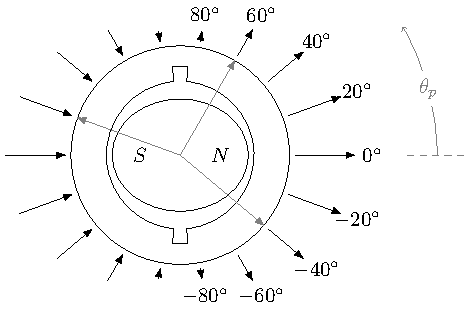
\includegraphics{figRotatingMachPrinciplesFluxVersusAngle}
\begin{tikzpicture}
%grid
%\draw[gray] (-\sRo,-\sRo) grid (\sRo,\sRo);
\stator{2}{90}
%elliptic rotor
\draw (-90:\rR-2*\gap) to [out=0,in=-90] (0:\rR) to [out=90,in=0] (90:\rR-2*\gap) to [out=180,in=90] (180:\rR) to [out=-90,in=180] (-90:\rR-2*\gap);
\draw node at (0:0.6*\rR){$N$};
\draw node at (180:0.6*\rR){$S$};
%flux
\foreach \angle in {-80,-60,...,80}{
\draw[-latex] (\angle:\sRo+\gap)--++(\angle:cos \angle) node[shift={(\angle:0.3)}] {$\angle\degree$};}
\foreach \angle in {100,120,...,260}{
\draw[latex-] (\angle:\sRo+\gap)--++(\angle:-cos \angle);}
%
\draw[gray,-latex] (0,0)--(-40:\sRo);
\draw[gray,-latex] (0,0)--(60:\sRo);
\draw[gray,-latex] (0,0)--(160:\sRo);
%
\draw[gray,dashed] (0:\sRo+2)--++(0:1);
\draw[gray,->] (0:\sRo+2.5) arc (0:30:\sRo+2.5);
\draw node[gray,fill=white] at (15:\sRo+2.5){$\theta_p$};
\end{tikzpicture}
\caption{کثافتِ مقناطیسی بہاو اور زاویہ کا تبدیلی۔}
\label{شکل_گھومتے_مشین_رداس_اور_مقناطیسی_بہاو}
\end{figure}

شکل  \حوالہ{شکل_گھومتے_مشین_رداس_اور_مقناطیسی_بہاو_مقناطیس_گھوما_ہے} میں مقناطیس اور اس کا سائن نما مقناطیسی دباو پیش کیا گیا ہے۔ جیسا شکل \حوالہ{شکل_گھومتے_مشین_مقناطیسی_دباو_سمتیہ}  میں دکھایا گیا ہے، ایسے مقناطیسی دباو کو عموماً ایک سمتیہ سے ظاہر کیا جاتا ہے جہاں سمتیہ کا طول مقناطیسی دباو کا حیطہ اور سمتیہ کا رخ مقناطیس کے شمال کو ظاہر کرتا ہے۔
\begin{figure}
\centering
%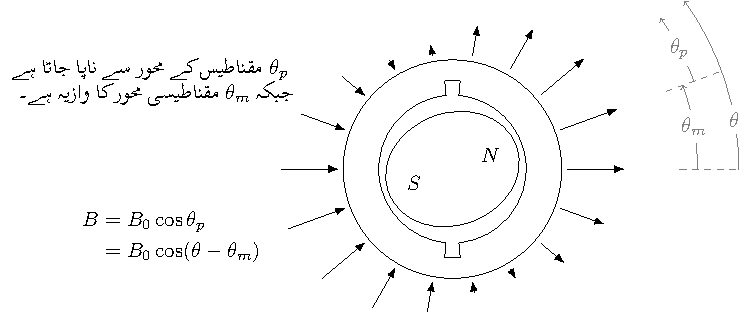
\includegraphics{figRotatingMachPrinciplesFluxVersusAngleTiltedRotor}
\begin{tikzpicture}
%grid
%\draw[gray] (-\sRo,-\sRo) grid (\sRo,\sRo);
\stator{2}{90}
%elliptic rotor
\begin{scope}[rotate=20]
\draw (-90:\rR-2*\gap) to [out=0,in=-90] (0:\rR) to [out=90,in=0] (90:\rR-2*\gap) to [out=180,in=90] (180:\rR) to [out=-90,in=180] (-90:\rR-2*\gap);
\draw node at (0:0.6*\rR){$N$};
\draw node at (180:0.6*\rR){$S$};
%flux
\foreach \angle in {-80,-60,...,80}{
\draw[-latex] (\angle:\sRo+\gap)--++(\angle:cos \angle) ;}
\foreach \angle in {100,120,...,260}{
\draw[latex-] (\angle:\sRo+\gap)--++(\angle:-cos \angle);}
%
\draw[gray,dashed] (0:\sRo+2)--++(0:1);
\draw[gray,->] (0:\sRo+2.5) arc (0:16:\sRo+2.5);
\draw node[gray,fill=white] at (8:\sRo+2.5){$\theta_p$};
\end{scope}
%
\draw[gray,dashed] (0:\sRo+2)--++(0:1);
\draw[gray,->] (0:\sRo+2.3) arc (0:20:\sRo+2.3);
\draw node[gray,fill=white] at (10:\sRo+2.3){$\theta_m$};
%
\draw[gray,dashed] (0:\sRo+2)--++(0:1);
\draw[gray,->] (0:\sRo+3) arc (0:36:\sRo+3);
\draw node[gray,fill=white] at (10:\sRo+3){$\theta$};
%text
\draw node[left,align=right] at (150:1.6*\sRo){\RL{ $\theta_p$ مقناطیس کے محور سے ناپا جاتا ہے}\\ \RL{اور $\theta_m$ مقناطیسی محور کا زاویہ ہے۔}};
\draw node[left] at (200:1.8*\sRo){$\begin{aligned}  B&=B_0 \cos \theta_p\\&=B_0 \cos (\theta-\theta_m)  \end{aligned}$};
\end{tikzpicture}
\caption{کثافت مقناطیسی بہاو اور مقناطیس کا زاویہ۔}
\label{شکل_گھومتے_مشین_رداس_اور_مقناطیسی_بہاو_مقناطیس_گھوما_ہے}
\end{figure}
%
\begin{figure}
\centering
%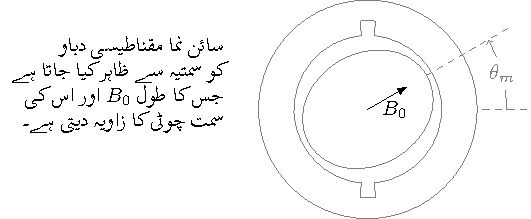
\includegraphics{figRotatingMachPrinciplesFluxVector}
\begin{tikzpicture}
%grid
%\draw[gray] (-\sRo,-\sRo) grid (\sRo,\sRo);
\begin{scope}[draw=gray]
\stator{2}{90}
\end{scope}
%elliptic rotor
\pgfmathsetmacro{\angle}{30}
\begin{scope}[rotate=\angle]
\draw[gray] (-90:\rR-2*\gap) to [out=0,in=-90] (0:\rR) to [out=90,in=0] (90:\rR-2*\gap) to [out=180,in=90] (180:\rR) to [out=-90,in=180] (-90:\rR-2*\gap);
%flux
\draw[-latex] (0,0) --(0:0.75)node [below,pos=0.7]{$B_0$};
\draw[gray,dashed] (0:\rR)--++(0:1.6);
\end{scope}
%
\draw[gray,dashed] (0:\sRo+0.1)--++(0:0.8);
\draw[gray,->] (0:\sRo+0.5) arc (0:\angle:\sRo+0.5);
\draw node[gray,fill=white] at (\angle/2:\sRo+0.5){$\theta_m$};
%text
\draw node[left,align=right] at (170:\sRo+0.5){\RL{سائن نما مقناطیسی دباو} \\  \RL{کو سمتیہ سے ظاہر کیا جاتا ہے} \\   \RL{جس کا  طول $B_0$ اور اس کا} \\  \RL{رخ چوٹی کا زاویہ دیتا ہے۔}}; 
\end{tikzpicture}
\caption{مقناطیسی دباو کو سمتیہ سے ظاہر کیا جاتا ہے۔}
\label{شکل_گھومتے_مشین_مقناطیسی_دباو_سمتیہ}
\end{figure}

 شکل \حوالہ{شکل_گھومتے_مشین_رداس_اور_مقناطیسی_بہاو_مقناطیس_گھوما_ہے}  میں مقناطیس کو لمحہ \عددیء{t_1}،  زاویہ \عددیء{\theta_m(t_1)} پر دکھایا گیا ہے جہاں ساکن لچھے کا ارتباط بہاو \عددیء{\lambda_\theta} ہے۔ اگر مقناطیس گھڑی کے مخالف رخ ایک مقررہ رفتار \عددیء{\omega_0} سے  گھوم رہا ہو تب ساکن لچھے میں اس لمحہ پر برقی دباو \عددیء{e(t)} پیدا ہو گا:
\begin{align}
e(t)=\frac{\dif \lambda_\theta}{\dif t}
\end{align}
آدھے چکر، \عددیء{\pi} ریڈیئن  گھومنے کے،  بعد  مقناطیسی  قطبین آپس میں جگہیں تبدیل کرتے ہیں، لچھے میں مقناطیسی بہاو کا رخ الٹ ہو گا،لچھے میں ارتباط بہاو \عددیء{-\lambda_\theta}  اور اس میں امالی برقی دباو \عددیء{-e(t)} ہو گا۔ایک مکمل چکر بعد مقناطیس  دوبارہ اسی مقام پر ہو گا جو شکل \حوالہ{شکل_گھومتے_مشین_رداس_اور_مقناطیسی_بہاو_مقناطیس_گھوما_ہے} میں دکھایا گیا ہے، ساکن لچھے کا ارتباط بہاو دوبارہ \عددیء{\lambda_\theta} اور اس میں امالی برقی دباو \عددیء{e(t)} ہو گا۔ یوں جب بھی مقناطیس  \عددیء{\theta_m=2\pi}  میکانی زاویہ طے کرے،  امالی برقی دباو کے  برقی زاویہ میں \عددیء{\theta_e=2\pi}  تبدیلی رونما ہو گی  لہٰذا دو قطب، ایک لچھے  کی مشین میں میکانی زاویہ \عددیء{\theta_m} اور برقی زاویہ \عددیء{\theta_e}  ایک دوسرے کے برابر ہوں گے:
\begin{align*}
\theta_e=\theta_m
\end{align*}
اس مشین میں اگر مقناطیس \عددیء{f_m} چکر فی سیکنڈ کی رفتار سے گھومتا ہو تب لچھے میں امالی برقی دباو \عددیء{e(t)} بھی ایک سیکنڈ میں \عددیء{f_m} مکمل چکر کاٹے گا لہٰذا  \عددیء{e(t)} کے \اصطلاح{تعدد}\فرہنگ{تعدد} \حاشیہب{frequency}\فرہنگ{frequency}\عددیء{f_e}   کی قیمت  \عددیء{f_m} ہرٹز\حاشیہب{Hertz} ہو گی۔
\begin{align*}
f_e=f_m
\end{align*}
%
\begin{figure}
\centering
%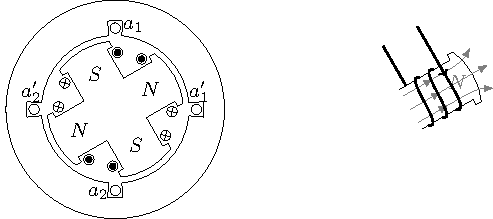
\includegraphics{figRotatingMachPrinciplesFourPoleFourSlotSynchronousMachine}
\begin{tikzpicture}
%grid
%\draw[gray] (-\sRo,-\sRo) grid (\sRo,\sRo);
\pgfmathsetmacro{\shiftX}{5cm}
\stator{4}{0}
\rotor{4}{30}

\slotEmptyCircle{0,90,180,270}
\slotName{0/a_1'/above,90/a_1/right,180/a_2'/above,270/a_2/left}
\dotCrossEachPole{30,210}
\crossDotEachPole{120,300}
\draw node at (30:0.6*\rR){$N$};
\draw node at (210:0.6*\rR){$N$};
\draw node at (120:0.6*\rR){$S$};
\draw node at (300:0.6*\rR){$S$};
%
\begin{scope}[xshift=\shiftX]
\pgfmathsetmacro{\rReduction}{0}   %reduction in rotor length due to adjacent rotor
\pgfmathsetmacro{\rWr}{1}    %rotor's flat section's effective length
\begin{scope}[rotate=30]
\draw(\rReduction,-\rT/2)--++(\rWr,0)--++(0,-\pY)--++(\pX,0)  arc (-\pTheta/2:\pTheta/2:\rR)--++(-\pX,0)--++(0,-\pY)--++(-\rWr,0);
\node[gray] at (0:0.8*\rR){$N$};
%flux
\draw[gray,-latex] (0,\rT/3)--++(0:0.5*\rR);
\draw[gray,-latex] (0,\rT/3)++(0:0.5*\rR)--++(0:0.3*\rR) to [out=0,in=210] (1.2*\rR,\rT/2);
\draw[gray,-latex] (0,0)--++(0:0.5*\rR);
\draw[gray,-latex] (0,0)++(0:0.5*\rR)--++(0:0.8*\rR);
\draw[gray,-latex] (0,-\rT/3)--++(0:0.5*\rR);
\draw[gray,-latex] (0,-\rT/3)++(0:0.5*\rR)--++(0:0.3*\rR) to [out=0,in=150] (1.2*\rR,-\rT/2);
\begin{scope}[rotate=-90]
%COIL
%left leg coil.  drawn from top to bottom
%======
\pgfmathsetmacro{\nL}{3}
\pgfmathsetmacro{\stepHL}{(\rWr-\pX-\gap)/(\nL)}
%
\def\leftEdge{-\rT/2};
\def\coilTop{\rWr-\pX-\gap};
\def\rightEdge{\rT/2};
%
\draw[thick](\leftEdge+\rT/4,\coilTop) to [out=0,in=45] (\rightEdge,{\coilTop-\stepHL/2}); %top half turn
%coil itself
\pgfmathsetmacro{\nLend}{\nL-2}
\foreach \y in { 0, ..., \nLend }{
\draw[thick] (\leftEdge,{\coilTop-\stepHL/2-\y*\stepHL}) to [out=-135,in=45] (\rightEdge,{\coilTop-\stepHL/2-\y*\stepHL-\stepHL});
} 
%left hand terminals
\draw[thick,<-] (\leftEdge+\rT/4,\coilTop)--++(-1.25*\rT,0) node(TA){};
\draw[thick] (\leftEdge,\coilTop-\nL*\stepHL+0.5*\stepHL)--++(-1*\rT,0)node(TB){};
%\node at ($(TA)!0.5!(TB)$){$\begin{aligned}&+\\ e&,\lambda\\&-   \end{aligned}$};
%=================================
\end{scope}
\end{scope}
\end{scope}
\end{tikzpicture}
\caption{چار قطب یک دوری معاصر جنریٹر۔}
\label{شکل_گھومتے_مشین_چار_قطب_معاصر_مژین}
\end{figure}


اس مشین میں  میکانی زاویہ \عددیء{\theta_m} اور برقی زاویہ \عددیء{\theta_e}  وقت کے ساتھ تبدیل ہونے کے باوجود آپس میں ایک تناسب رکھتے ہیں لہٰذا ایسے مشین کو \اصطلاح{معاصر} مشین\فرہنگ{معاصر}\حاشیہب{synchronous machine}\فرہنگ{synchronous}  کہتے ہیں۔ یہاں یہ تناسب ایک کے برابر ہے۔ 

شکل \حوالہ{شکل_گھومتے_مشین_چار_قطب_معاصر_مژین}  میں چار قطب، یک دوری معاصر جنریٹر دکھایا گیا ہے۔ چھوٹے مشینوں میں عموماً مقناطیس جبکہ بڑے مشینوں میں \اصطلاح{برقی مقناطیس}\فرہنگ{مقناطیس!برقی}\حاشیہب{electromagnet}\فرہنگ{electromagnet} استعمال ہوتے ہیں۔ اس شکل میں  برقی مقناطیس استعمال کیے گئے ہیں۔ دو سے زائد قطبین والے مشینوں میں کسی ایک شمالی قطب کو حوالہ قطب تصور کیا جاتا ہے۔ شکل میں اس حوالہ قطب کو \عددیء{\theta_m} پر دکھایا گیا ہے اور یوں دوسرا شمالی قطب \عددیء{(\theta_m+\pi)}  زاویہ پر ہے۔

 جیسا کہ نام سے واضح ہے، اس مشین میں  مقناطیس کے چار قطبین  ہیں۔ ہر ایک شمالی قطب کے بعد ایک جنوبی قطب آتا ہے۔ یک دوری آلات میں مقناطیسی  قطبین کے جوڑوں کی تعداد اور ساکن لچھوں کی تعداد ایک دوسرے کے برابر ہوتی ہے۔ شکل \حوالہ{شکل_گھومتے_مشین_چار_قطب_معاصر_مژین}  میں  مشین کے چار قطب یعنی دو جوڑی قطبین ہیں،  لہٰذا اس مشین کے ساکن حصہ پر دو ساکن لچھے ہوں ہیں۔ ایک لچھے کو \عددیء{a_1} سے واضح کیا گیا ہے اور دوسرے کو \عددیء{a_2} سے۔لچھے \عددیء{a_1} کو  قالب میں موجود دو شگاف \عددیء{a_1} اور \عددیء{a_1'} میں لپیٹا گیا ہے۔ اسی طرح \عددیء{a_2} لچھے کو دو شگاف \عددیء{a_2} اور \عددیء{a_2'} میں رکھا گیا ہے۔ ان دونوں لچھوں میں یکساں برقی دباو پیدا ہوتا ہے۔  دونوں لچھوں کو سلسلہ وار\حاشیہب{series connected} جوڑا جاتا ہے۔ اس طرح جنریٹر سے حاصل برقی دباو ایک لچھے میں پیدا  برقی دباو کا دگنا ہو گا۔یک دوری آلات میں  قالب کو مقناطیس کے  قطبین کی تعداد کے برابر  حصوں میں تقسیم کرنے سے  مشین کا ہر ساکن لچھا ایک حصہ گھیرتا ہے۔ شکل \حوالہ{شکل_گھومتے_مشین_چار_قطب_معاصر_مژین} میں چار  قطبین  ہیں  لہٰذا اس کا ایک لچھا  نوے میکانی زاویہ کے احاطے کو گھیرتا ہے۔

ساکن اور حرکی لچھوں کی کارکردگی ایک دوسرے سے مختلف ہوتی ہے۔اس کی  وضاحت کرتے ہیں۔

جیسا پہلے بھی ذکر کیا گیا چھوٹی گھومتی مشینوں میں مقناطیسی میدان ایک مقناطیس  فراہم کرتا ہے جبکہ بڑی مشینوں میں برقی مقناطیس  میدان فراہم کرتا ہے۔اگرچہ اب تک کی اشکال میں مقناطیس کو گھومتا حصہ دکھایا گیا ہے، حقیقت میں مقناطیس  کسی مشین میں گھومتا اور کسی میں  ساکن ہو گا۔ میدان فراہم کرنے والا لچھا مشین کے کل برقی طاقت کے چند فی صد برابر برقی طاقت استعمال کرتا ہے۔میدان فراہم کرنے والے اس لچھے کو \اصطلاح{میدانی لچھا}\فرہنگ{لچھا!میدانی}\حاشیہب{field coil}\فرہنگ{field coil}  کہتے ہیں۔اس کے برعکس مشین میں موجود دوسری نوعیت کے لچھے کو \اصطلاح{قوی لچھا}\فرہنگ{لچھا!قوی}\حاشیہب{armature coil}\فرہنگ{armature coil}  کہتے ہیں۔برقی جنریٹر کے قوی لچھے سے  برقی طاقت  حاصل کی جاتی ہے ۔برقی موٹروں میں میدانی لچھے میں چند فی صد برقی طاقت کے ضیاع کے علاوہ  تمام برقی طاقت  قوی لچھے کو فراہم کی جاتی ہے۔
\begin{figure}
\centering
\begin{minipage}{0.45\textwidth}
\centering
%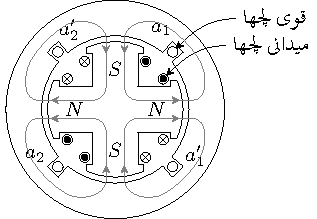
\includegraphics{figRotatingMachPrinciplesFourPoleTwoCoilFlux}
\begin{tikzpicture}
\pgfmathsetmacro{\shiftX}{5cm}
\stator{4}{45}
\rotor{4}{0}

\slotEmptyCircle{45,135,-45,-135}
\dotCrossEachPole{0,180}
\crossDotEachPole{90,270}
\draw node at (0:0.6*\rR){$N$};
\draw node at (180:0.6*\rR){$N$};
\draw node at (90:0.6*\rR){$S$};
\draw node at (270:0.6*\rR){$S$};
%
%\slotName{45/a_1/,-45/a_1'/below,135/a_2'/,-135/a_2/below}
\draw (45+15:\sRi+1.25*\delR)node[]{$a_1$};
\draw (135-15:\sRi+1.25*\delR)node[]{$a_2'$};
\draw (-45+15:\sRi+1.25*\delR)node[]{$a_1'$};
\draw (-135-15:\sRi+1.25*\delR)node[]{$a_2$};
%text
\draw[stealth-] (45:\sRi cm+1/2*\delR cm+2.5pt) to [out=45,in=180] ++(1cm,0.5cm)node[right]{\RL{قوی لچھا}};
\draw[stealth-] (\rWf -\pX -1.3*\pX ,\rT/2 +1.3*\pX  )++(45:2.5pt) to [out=45,in=180] ++(1cm,0.5cm)node[right]{\RL{میدانی لچھا}};
%===========================
%FLUX 0degree to 90 degree
\pgfmathsetmacro{\delAngle}{30}   %smooth flux entry into stator
\draw[gray,-stealth] (\rT/2,\rT/5)coordinate(aa)--++(0:0.6*\rR);
\draw[gray](\rT/2,\rT/5)++(0:0.6*\rR)--++(0:0.2*\rR) to [out=0,in=-90+\delAngle] (\delAngle:\sRo-0.2) arc (\delAngle:90-\delAngle:\sRo-0.2)coordinate (leftUpperFlux);
\draw[gray] (\rT/5,\rT/2)coordinate(bb)--++(90:0.5*\rR);
\draw[gray,stealth-](\rT/5,\rT/2)++(90:0.5*\rR)--++(90:0.2*\rR) to [out=90,in=180-\delAngle] (leftUpperFlux);
\draw[gray] (bb) to [out=-90,in=180] (aa);
%====
%FLUX 0 degree to -90 degree
\draw[gray,-stealth] (\rT/2,-\rT/5)coordinate(aa)--++(0:0.6*\rR);
\draw[gray](\rT/2,-\rT/5)++(0:0.6*\rR)--++(0:0.2*\rR) to [out=0,in=90-\delAngle] (-\delAngle:\sRo-0.2) arc (-\delAngle:-90+\delAngle:\sRo-0.2)coordinate (leftUpperFlux);
\draw[gray] (\rT/5,-\rT/2)coordinate(bb)--++(-90:0.5*\rR);
\draw[gray,stealth-](\rT/5,-\rT/2)++(-90:0.5*\rR)--++(-90:0.2*\rR) to [out=-90,in=180+\delAngle] (leftUpperFlux);
\draw[gray] (bb) to [out=90,in=180] (aa);
%====
%FLUX 90 degree to 180 degree
\draw[gray,-stealth] (-\rT/2,\rT/5)coordinate(aa)--++(180:0.6*\rR);
\draw[gray](-\rT/2,\rT/5)++(180:0.6*\rR)--++(180:0.2*\rR) to [out=180,in=-90-\delAngle] (180-\delAngle:\sRo-0.2) arc (180-\delAngle:90+\delAngle:\sRo-0.2)coordinate (leftUpperFlux);
\draw[gray] (-\rT/5,\rT/2)coordinate(bb)--++(90:0.5*\rR);
\draw[gray,stealth-](-\rT/5,\rT/2)++(90:0.5*\rR)--++(90:0.2*\rR) to [out=90,in=\delAngle] (leftUpperFlux);
\draw[gray] (bb) to [out=-90,in=0] (aa);
%====
%FLUX -90 degree to 180 degree
\draw[gray,-stealth] (-\rT/2,-\rT/5)coordinate(aa)--++(180:0.6*\rR);
\draw[gray](-\rT/2,-\rT/5)++(180:0.6*\rR)--++(180:0.2*\rR) to [out=180,in=90+\delAngle] (180+\delAngle:\sRo-0.2) arc (180+\delAngle:270-\delAngle:\sRo-0.2)coordinate (leftUpperFlux);
\draw[gray] (-\rT/5,-\rT/2)coordinate(bb)--++(-90:0.5*\rR);
\draw[gray,stealth-](-\rT/5,-\rT/2)++(-90:0.5*\rR)--++(-90:0.2*\rR) to [out=-90,in=-\delAngle] (leftUpperFlux);
\draw[gray] (bb) to [out=90,in=0] (aa);
\end{tikzpicture}
\caption{چار قطب، دو لچھے مشین میں مقناطیسی بہاو۔}
\label{شکل_گھومتے_مشین_چار_قطب_کا_بہاو}
\end{minipage}%
\begin{minipage}{0.45\textwidth}
\centering
%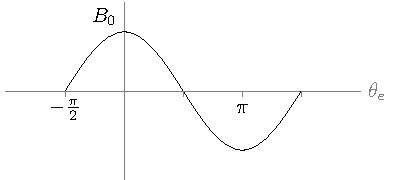
\includegraphics{figRotatingMachPrinciplesCosineFlux}
\begin{tikzpicture}[declare function={f(\x)=cos(\x);}]
\begin{axis}[small,axis lines=middle,xlabel={$\theta_e$},xtick={-90,180},xticklabels={$-\tfrac{\pi}{2}$,$\pi$},ytick={1},yticklabels={$B_0$},enlargelimits=true,xlabel style={at={(current axis.right of origin)},anchor=north}]
\addplot[domain=-90:270,smooth]{f(x)};
%grid
%\draw[gray] (-\sRo,-\sRo) grid (\sRo,\sRo);
%\draw[gray](-2,0) --(4,0)node[right]{$\theta_e$}; %axis
%\draw[gray] (0,-1.5)--(0,1.5);
%\draw[above left] node at (0,1){$B_0$};
%\draw (0,1) cos (-1,0) node[below]{$-\tfrac{\pi}{2}$};
%\draw (0,1) cos (1,0);
%\draw (2,-1) cos (1,0);
%\draw (2,-1) cos (3,0);
%\foreach \x in {-1,1,2,3}{
%\draw[gray](\x,0)--++(0,-0.1);}
%\draw[gray](2,0)--++(0,-0.1)node[below,text=black]{$\pi$};
\end{axis}
\end{tikzpicture}
\caption{سائن نما کثافتِ مقناطیسی بہاو۔}
\label{شکل_گھومتے_مشین_سائن_نما_بہاو}
\end{minipage}%
\end{figure}



شکل \حوالہ{شکل_گھومتے_مشین_چار_قطب_کا_بہاو} میں گھومتے اور ساکن حصہ کے بیچ خلائی درز میں  شمالی قطب سے مقناطیسی بہاو باہر نکل کر  قالب میں داخل ہوتا ہے جبکہ جنوبی قطب پر مقناطیسی بہاو قالب سے نکل کر جنوبی قطب میں  داخل ہوتا ہے۔ شکل \حوالہ{شکل_گھومتے_مشین_چار_قطب_کا_بہاو}  میں اس مقناطیسی بہاو کی کثافت کو دکھایا گیا ہے۔ یوں اگر ہم اس خلائی درز میں ایک گول چکر کاٹیں تو مقناطیسی بہاو کا رخ  دو مرتبہ باہر کی جانب اور دو مرتبہ اندر کی جانب ہو گا۔ ان مشینوں  میں کوشش کی جاتی ہے کہ خلائی درز میں \عددیء{B} سائن نما ہو۔ یہ کیسے کیا جاتا ہے، اس پر آگے غور کیا جائے گا۔ اگر تصور کر لیا جائے کہ \عددیء{B} سائن نما ہے تب  خلائی درز میں \عددیء{B} کی مطلق قیمت شکل \حوالہ{شکل_گھومتے_مشین_سائن_نما_بہاو}  کی طرح ہو گی جہاں \عددیء{\theta_e} برقی زاویہ ہے۔ 

\عددیء{P} قطبی مقناطیس کے معاصر مشین  کے لئے لکھ درج ذیل ہو گا۔
\begin{align}
\theta_e&=\frac{P}{2} \theta_m\label{مساوات_گھومتے_مشین_برقی_میکانی_زاویہ_تعلق}\\
f_e&=\frac{P}{2} f_m  \label{مساوات_گھومتے_مشین_برقی_میکانی_تعدد_تعلق}
\end{align}
یہاں برقی اور میکانی  تعدد کا تناسب \عددی{2} ہے۔ 
%
\ابتدا{مثال}
پاکستان میں گھریلو اور صنعتی صارفین کو \عددیء{\SI{50}{\hertz}} کی برقی طاقت فراہم کی جاتی ہے۔یوں ہمارے ہاں \عددیء{f_e=50} ہو گا۔
\begin{itemize}
\item
اگر برقی طاقت دو قطبی جنریٹر سے حاصل کی جائے تب جنریٹر  کی رفتار کتنی ہو گی؟۔
\item
اگر جنریٹر کے بیس قطب ہوں تب  جنریٹر کی رفتار کتنی ہو گی؟
\end{itemize}

حل:\quad
\begin{itemize}
\item
مساوات \حوالہ{مساوات_گھومتے_مشین_برقی_میکانی_تعدد_تعلق}  کے تحت دو قطبی،\عددیء{P=2}،  جنریٹر کا میکانی رفتار  
\عددیء{f_m=\tfrac{2}{2}(50)=50} چکر فی سیکنڈ یعنی \عددیء{3000} چکر فی منٹ\حاشیہب{rpm, rounds per minute} ہو گا۔
\item
بیس قطبی، \عددیء{P=20}،  جنریٹر  کا میکانی رفتار \عددیء{f_m=\tfrac{2}{20}(50)=5} چکر فی سیکنڈ یعنی \عددیء{300} چکر فی منٹ ہو گا۔
\end{itemize}
\انتہا{مثال}
%

 اب یہ فیصلہ کس طرح کیا جائے کہ جنریٹر کے قطب کتنے رکھے جائیں۔ درحقیقت پانی سے چلنے والے جنریٹر سست رفتار جبکہ ٹربائن سے چلنے والے جنریٹر تیز رفتار ہوتے ہیں، لہٰذا پانی سے چلنے والے جنریٹر زیادہ قطب رکھتے ہیں جبکہ ٹربائن سے چلنے والے جنریٹر عموماً دو قطب کے ہوتے ہیں۔
\begin{figure}
\centering
%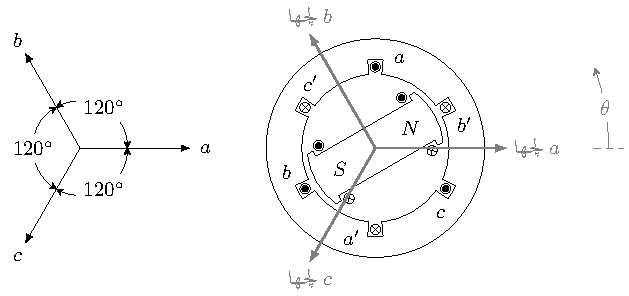
\includegraphics{figRotatingMachPrinciplesTwoPoleThreePhase}
\begin{subfigure}{0.60\textwidth}
\centering
\begin{tikzpicture}
\stator{6}{30}
\slotDot{90,-30,210}
\slotCross{-90,30,150}
\rotor{2}{30}
\dotCrossEachPole{30}
\crossDotEachPole{210}
\draw node at (30:0.6*\rR){$N$};
\draw node at (210:0.6*\rR){$S$};
%
%\slotName{45/a_1/,-45/a_1'/below,135/a_2'/,-135/a_2/below}
\draw (90-15:\sRi+1.25*\delR)node[]{$a$};
\draw (270-15:\sRi+1.25*\delR)node[]{$a'$};
\draw (210-15:\sRi+1.25*\delR)node[]{$b$};
\draw (30-15:\sRi+1.25*\delR)node[]{$b'$};
\draw (-30-15:\sRi+1.25*\delR)node[]{$c$};
\draw (150-15:\sRi+1.25*\delR)node[]{$c'$};
%
\draw[thick,gray,-latex](0,0)--(0:1.2*\sRo)node[right]{\RL{$a$ لچھا}};
\draw[thick,gray,-latex](0,0)--(120:1.2*\sRo)node[above]{\RL{$b$ لچھا}};
\draw[thick,gray,-latex](0,0)--(-120:1.2*\sRo)node[below]{\RL{$c$ لچھا}};
%text
\draw[thin,gray,dashed] (0:2*\sRo)--++(0.25,0)coordinate(zeroAngle)--++(0.25,0);
\draw[gray,-stealth] (zeroAngle) arc (0:20:2*\sRo+0.25);
\node[fill=white,text=gray] at (10:2*\sRo+0.25){$\theta$};
\end{tikzpicture}
\end{subfigure}%
\begin{subfigure}{0.35\textwidth}
\centering
\begin{tikzpicture}
\draw[-latex](0,0)--(0:1*\sRo)node[shift={(0:1*\sRo+0.2cm)}]{$a$};
\draw[-latex](0,0)--(120:1*\sRo)node[shift={(120:1*\sRo+0.2cm)}]{$b$};
\draw[-latex](0,0)--(-120:1*\sRo)node[shift={(-120:1*\sRo+0.2cm)}]{$c$};
%
\draw[stealth-stealth]([shift={(0:0.8)}]0,0)  arc (0:120:0.8);
\draw node at (60:0.8)[fill=white]{$120\degree$};
\draw[stealth-stealth]([shift={(0:0.8)}]0,0)  arc (0:-120:0.8);
\draw node at (-60:0.8)[fill=white]{$120\degree$};
\draw[stealth-stealth]([shift={(120:0.8)}]0,0)  arc (120:240:0.8);
\draw node at (180:0.8)[fill=white]{$120\degree$};
\end{tikzpicture}
\end{subfigure}%
\caption{دو قطب، تین دوری معاصر مشین۔}
\label{شکل_گھومتے_مشین_دو_قطب_تین_دور_معاصر}
\end{figure}

شکل \حوالہ{شکل_گھومتے_مشین_دو_قطب_تین_دور_معاصر}  میں دو قطب  تین دوری معاصر مشین دکھایا گیا ہے۔اس میں تین ساکن لچھے ہیں۔ان میں ایک لچھا \عددیء{a} ہے جو قالب میں  شگاف  \عددیء{a} اور \عددیء{a'} میں رکھا گیا ہے۔ اگر اس شکل میں باقی دو لچھے نہ ہوتے تب یہ بالکل شکل \حوالہ{شکل_گھومتے_مشین_دو_قطب_ایک_دور_معاصر_بنیادی_شکل}  میں دیا گیا مشین ہی تھا۔البتہ دیے گئے شکل میں ایک کی بجائے تین ساکن لچھے ہیں۔

لچھے کا رخ\فرہنگ{لچھا!رخ} درج ذیل طریقہ سے تعین کیا جاتا ہے۔

\begin{itemize}
\item
دائیں ہاتھ کی چار انگلیوں کو دونوں شگافوں میں برقی رو کے رخ لپیٹیں۔ دائیں ہاتھ کا انگوٹھا لچھے کا رخ دے گا۔
\end{itemize}

 شکل \حوالہ{شکل_گھومتے_مشین_دو_قطب_تین_دور_معاصر} میں  لچھا \عددیء{a}   کا برقی رو  شگاف \عددیء{a} میں،  کتاب کے صفحہ کو عمودی،  باہر رخ جبکہ  \عددیء{a'}  میں اس کے مخالف اندر رخ تصور کرتے ہوئے  لچھا \عددیء{a} کا رخ تیر دار لکیر سے دکھایا گیا ہے۔ اس رخ کو ہم صفر زاویہ تصور کرتے ہیں۔ یوں لچھا \عددیء{a}  صفر زاویہ پر لپیٹا گیا ہے، یعنی \عددیء{\theta_a=0\degree} ہے۔ باقی لچھوں کے زاویات   لچھا \عددیء{a} کے رخ سے، گھڑی کے مخالف رُخ ناپے جاتے ہیں۔

شکل \حوالہ{شکل_گھومتے_مشین_دو_قطب_تین_دور_معاصر}  میں لچھا \عددیء{b} کو شگاف \عددیء{b} اور \عددیء{b'} میں رکھا گیا ہے اور لچھا \عددیء{c} کو شگاف \عددیء{c} اور \عددیء{c'} میں رکھا گیا ہے۔ مزید  لچھا \عددیء{b} کو \عددیء{120\degree}  زاویہ اور لچھا \عددیء{c} کو \عددیء{240\degree} زاویہ پر رکھا گیا ہے۔ یوں \عددیء{\theta_b=120\degree} اور \عددیء{\theta_c=240\degree} ہوں گے۔
\begin{figure}
\centering
%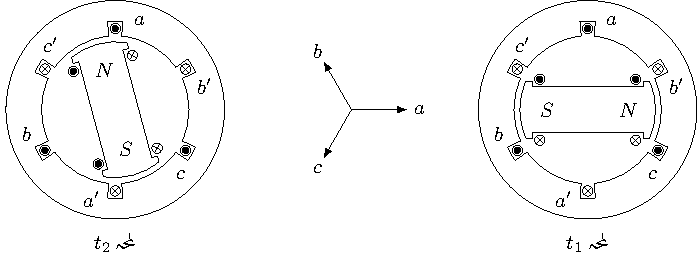
\includegraphics{figRotatingMachPrinciplesTwoPoleThreePhaseTwoMoments}
\begin{subfigure}{0.40\textwidth}
\centering
\begin{tikzpicture}
\stator{6}{30}
\slotDot{90,-30,210}
\slotCross{-90,30,150}
\rotor{2}{0}
\dotCrossEachPole{00}
\crossDotEachPole{180}
\draw node at (0:0.6*\rR){$N$};
\draw node at (180:0.6*\rR){$S$};
%
%\slotName{45/a_1/,-45/a_1'/below,135/a_2'/,-135/a_2/below}
\draw (90-15:\sRi+1.25*\delR)node[]{$a$};
\draw (270-15:\sRi+1.25*\delR)node[]{$a'$};
\draw (210-15:\sRi+1.25*\delR)node[]{$b$};
\draw (30-15:\sRi+1.25*\delR)node[]{$b'$};
\draw (-30-15:\sRi+1.25*\delR)node[]{$c$};
\draw (150-15:\sRi+1.25*\delR)node[]{$c'$};
%text
\node at (-90:\sRo+0.4){\RL{لمحہ $t_1$}};
\end{tikzpicture}
\end{subfigure}%
\begin{subfigure}{0.20\textwidth}
\centering
\begin{tikzpicture}
\draw[-latex](0,0)--(0:0.5*\sRo)node[shift={(0:0.5*\sRo+0.2cm)}]{$a$};
\draw[-latex](0,0)--(120:0.5*\sRo)node[shift={(120:0.5*\sRo+0.2cm)}]{$b$};
\draw[-latex](0,0)--(-120:0.5*\sRo)node[shift={(-120:0.5*\sRo+0.2cm)}]{$c$};
\end{tikzpicture}
\end{subfigure}%
\begin{subfigure}{0.40\textwidth}
\centering
\begin{tikzpicture}
\stator{6}{30}
\slotDot{90,-30,210}
\slotCross{-90,30,150}
\rotor{2}{120}
\dotCrossEachPole{120}
\crossDotEachPole{300}
\draw node at (120:0.6*\rR){$N$};
\draw node at (300:0.6*\rR){$S$};
%
%\slotName{45/a_1/,-45/a_1'/below,135/a_2'/,-135/a_2/below}
\draw (90-15:\sRi+1.25*\delR)node[]{$a$};
\draw (270-15:\sRi+1.25*\delR)node[]{$a'$};
\draw (210-15:\sRi+1.25*\delR)node[]{$b$};
\draw (30-15:\sRi+1.25*\delR)node[]{$b'$};
\draw (-30-15:\sRi+1.25*\delR)node[]{$c$};
\draw (150-15:\sRi+1.25*\delR)node[]{$c'$};
%text
\node at (-90:\sRo+0.4){\RL{لمحہ $t_2$}};
\end{tikzpicture}
\end{subfigure}%
\caption{دو قطب تین دوری مشین۔}
\label{شکل_گھومتے_مشین_دو_قطب_تین_دور_مختلف_لمحات}
\end{figure}

 شکل \حوالہ{شکل_گھومتے_مشین_دو_قطب_تین_دور_مختلف_لمحات}  میں اگر لمحہ \عددیء{t_1} پر  لچھا \عددیء{a} کا  ارتباط بہاو \عددیء{\lambda_a(t_1)} ہو تب لمحہ \عددیء{t_2} پر، جب مقناطیس \عددیء{120\degree} زاویہ طے کر لے،   لچھا \عددیء{b} کا ارتباط بہاو \عددیء{\lambda_b(t_2)} ہو گا۔  لمحہ \عددیء{t_2} پر مقناطیس اور لچھا \عددیء{b} ایک دوسرے کے لحاظ سے بالکل اسی طرح نظر آتے  ہیں جیسے \عددیء{t_1} پر مقناطیس اور لچھا \عددیء{a} ایک دوسرے کے لحاظ سے نظر آتے تھے۔ یوں لمحہ \عددیء{t_2} پر لچھا \عددیء{b} کا ارتباط بہاو  اتنا ہی ہو گا جتنا لمحہ \عددیء{t_1} پر  \عددیء{a} لچھا کا ارتباط بہاو تھا:
\begin{align}
\lambda_b(t_2)=\lambda_a(t_1)
\end{align}
اسی طرح  لمحہ \عددیء{t_3} پر، جب مقناطیس مزید  \عددیء{120\degree} زاویہ طے کر لے، لچھا \عددیء{c} کا ارتباط بہاو  \عددیء{\lambda_c(t_3)} ہو گا جو \عددیء{\lambda_a(t_1)} کے برابر ہو گا۔یوں درج ذیل لکھا جا سکتا ہے۔
\begin{align}\label{مساوات_گھومتے_مشین_مختلف_اوقات_پر_تین_لچھے_یکساں}
\lambda_c(t_3)=\lambda_b(t_2)=\lambda_a(t_1)
\end{align}
ان لمحات پر  لچھوں کے امالی برقی دباو
\begin{align}
e_a(t_1)&=\frac{\dif \lambda_a(t_1)}{\dif t}\\
e_b(t_2)&=\frac{\dif \lambda_b(t_2)}{\dif t}\\
e_c(t_3)&=\frac{\dif \lambda_c(t_3)}{\dif t}
\end{align}
ہوں گے۔ مساوات \حوالہ{مساوات_گھومتے_مشین_مختلف_اوقات_پر_تین_لچھے_یکساں}    کی روشنی میں درج ذیل ہو گا۔
\begin{align}\label{مساوات_گھومتے_مشین_تین_لمحات_دباو_یکساں}
e_a(t_1)=e_b(t_2)=e_c(t_3)
\end{align} 

اگر شکل \حوالہ{شکل_گھومتے_مشین_دو_قطب_تین_دور_مختلف_لمحات} میں صرف لچھا \عددیء{a} پایا جاتا تب یہ بالکل شکل \حوالہ{شکل_گھومتے_مشین_دو_قطب_ایک_دور_معاصر_بنیادی_شکل}   کی طرح ہوتا اور اگر ایسی صورت  میں مقناطیس  گھڑی کے مخالف رخ ایک مقررہ رفتار \عددیء{\omega_0} سے گھمایا جاتا تب، جیسے پہلے تذکرہ کیا گیا ہے، لچھا \عددیء{a} میں سائن نما برقی دباو پیدا ہوتا۔شکل \حوالہ{شکل_گھومتے_مشین_دو_قطب_تین_دور_مختلف_لمحات}  میں کسی ایک لچھے کو کسی دوسرے لچھے پر کوئی برتری حاصل نہیں ہے۔ یوں اگر شکل \حوالہ{شکل_گھومتے_مشین_دو_قطب_تین_دور_مختلف_لمحات}  میں  مقناطیس اسی طرح گھمایا جائے تب  تینوں ساکن لچھوں میں سائن نما برقی دباو پیدا ہو گا البتہ مساوات \حوالہ{مساوات_گھومتے_مشین_تین_لمحات_دباو_یکساں}    کے تحت یہ برقی دباو آپس میں  \عددیء{120\degree}  زاویہ پر ہوں گے۔


\begin{figure}
\centering
%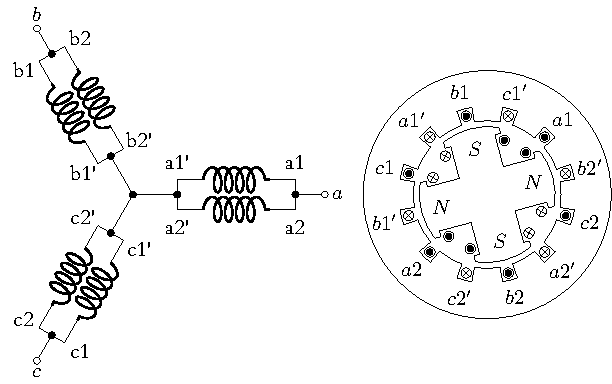
\includegraphics{figRotatingMachPrinciplesThreePhaseFourPole}
\begin{subfigure}{0.40\textwidth}
\centering
\begin{tikzpicture}
\pgfmathsetmacro{\shiftX}{5cm}
\pgfmathsetmacro{\sRo}{2.1}  %stator outer radius needs to be increased to accomodate the slot names
\pgfmathsetmacro{\sTilt}{45}  %stator tilt
\stator{12}{\sTilt}
%
\slotDot{\sTilt,\sTilt+60,\sTilt+120}       %a1,b1,c1
\slotCross{\sTilt+90,\sTilt+60+90,\sTilt+30}   %a1',b1',c1'
%\slotNameAtRadial{comma separated angles/name}
\slotNameAtRadial{\sTilt/a1,\sTilt+60/b1,\sTilt+120/c1}       %a1,b1,c1
\slotNameAtRadial{\sTilt+90/a1',\sTilt+60+90/b1',\sTilt+30/c1'}    %a1',b1',c1'
%
\pgfmathsetmacro{\sTilt}{45+180}  %stator tilt
\slotDot{\sTilt,\sTilt+60,\sTilt+120}       %a2,b2,c2
\slotCross{\sTilt+90,\sTilt+60+90,\sTilt+30}   %a2',b2',c2'
%\slotNameAtRadial{comma separated angles/name}
\slotNameAtRadial{\sTilt/a2,\sTilt+60/b2,\sTilt+120/c2}       %a2,b2,c2
\slotNameAtRadial{\sTilt+90/a2',\sTilt+60+90/b2',\sTilt+30/c2'}    %a2',b2',c2'

\rotor{4}{15}
%\dotCrossEachPole{comma separated poles}
\dotCrossEachPole{15,15+180}
\crossDotEachPole{15+90,15+90+180}
\draw node at (15:0.7*\rR){$N$};
\draw node at (15+180:0.7*\rR){$N$};
\draw node at (15+90:0.7*\rR){$S$};
\draw node at (15+90+180:0.7*\rR){$S$};
\end{tikzpicture}%
\end{subfigure}%
\begin{subfigure}{0.50\textwidth}
\centering
\begin{tikzpicture}
\draw (0,0) to [short,*-*] ++(0:0.75) to [short] ++(0,0.25)node[shift={(0+90:0.3)}]{a1'} to [inductor] ++(0:2)node[shift={(0+90:0.3)}]{a1} to [short,-*] ++(0,-0.25) to [short,-o] ++(0:0.5) node[right] {$a$};
\draw (0:0.75) to [short] ++(0,-0.25)node[shift={(0-90:0.3)}]{a2'} to [inductor] ++(0:2)node[shift={(0-90:0.3)}]{a2} to [short] ++(0,0.25);
%
\draw (0,0) to [short,-*] ++(120:0.75) to [short] ++(120+90:0.25)node[shift={(120+90:0.3)}]{b1'} to [inductor] ++(120:2)node[shift={(120+90:0.3)}]{b1} to [short,-*] ++(120-90:0.25) to [short,-o] ++(120:0.5) node [above]{$b$};
\draw (120:0.75) to [short] ++(120-90:0.25)node[shift={(120-90:0.3)}]{b2'} to [inductor] ++(120:2)node[shift={(120-90:0.3)}]{b2} to [short] ++(120+90:0.25);
%
\draw (0,0) to [short,-*] ++(240:0.75) to [short] ++(240+90:0.25)node[shift={(240+90:0.3)}]{c1'} to [inductor] ++(240:2)node[shift={(240+90:0.3)}]{c1} to [short,-*] ++(240-90:0.25) to [short,-o] ++(240:0.5)node[below]{$c$};
\draw (240:0.75) to [short] ++(240-90:0.25)node[shift={(240-90:0.3)}]{c2'} to [inductor] ++(240:2)node[shift={(240-90:0.3)}]{c2} to [short] ++(240+90:0.25);
\end{tikzpicture}
\end{subfigure}%
\caption{چار قطب، تین دوری معاصر مشین۔}
\label{شکل_گھومتے_مشین_چار_قطب_تین_دور_معاصر}
\end{figure}
شکل \حوالہ{شکل_گھومتے_مشین_چار_قطب_تین_دور_معاصر} میں چار قطب، تین دوری معاصر مشین دکھایا گیا ہے۔گھومتے حصے پر شمالی اور جنوبی قطبین باری باری پائے جاتے ہیں اور \عددیء{180\degree} میکانی زاویہ میں شمال اور قریبی جنوب قطب کی ایک  جوڑی  پائی جاتی ہے۔یہی میکانی زاویہ  \عددیء{360\degree} برقی زاویہ کے برابر ہو گا۔ شکل \حوالہ{شکل_گھومتے_مشین_دو_قطب_تین_دور_معاصر} میں ساکن حصہ کے \عددیء{360\degree} برقی زاویہ کے احاطہ میں تین دوری لچھے نسب  ہیں  جن کی اطراف کی ترتیب، گھڑی کے مخالف رخ چلتے ہوئے،   \عددیء{a}، \عددیء{c'}، \عددیء{b}، \عددیء{a'}، \عددیء{c} اور \عددیء{b'} ہے۔شکل \حوالہ{شکل_گھومتے_مشین_چار_قطب_تین_دور_معاصر} میں  دو قطبین کے احاطہ، \عددیء{180\degree} میکانی زاویہ (یا \عددی{360\degree} برقی زاویہ)، میں بالکل اسی طرح تین دوری لچھوں کے اطراف کی ترتیب   \عددیء{a1}، \عددیء{c1'}، \عددیء{b1}، \عددیء{a1'}، \عددیء{c1} اور \عددیء{c1'} ہے۔باقی دو قطبین کے احاطے میں بھی بالکل اسی طرح آپ کو \عددیء{a2}، \عددیء{c2'}، \عددیء{b2}،\عددیء{a2'}، \عددیء{c2} اور \عددیء{c2'} نظر آئیں گے۔کسی بھی لمحہ \عددیء{a1} اور \عددیء{a2} لچھوں میں بالکل یکساں برقی دباو پیدا ہو گا۔تین  دوری دو یکساں لچھوں کو سلسلہ وار یا متوازی جوڑ کر تین دوری برقی دباو حاصل کا جاتا ہے۔شکل \حوالہ{شکل_گھومتے_مشین_چار_قطب_تین_دور_معاصر} میں انہیں متوازی جوڑ کر دکھایا گیا ہے جہاں \عددیء{a} لچھے کو صفر زاویہ پر تصور کیا گیا ہے۔    

\حصہ{محرک برقی دباو}\شناخت{حصہ_گھومتے_مشین_محرک_برقی_دباو}
قانون لورینز\فرہنگ{قانون!لورینز}\حاشیہب{Lorentz law}\فرہنگ{Lorentz law} کے تحت مقناطیسی میدان \سمتیہ{B} میں سمتی رفتار \سمتیہ{v} سے حرکت پذیر  \اصطلاح{برقی بار}\فرہنگ{برقی بار}\فرہنگ{بار}\حاشیہب{charge}\فرہنگ{charge}  \عددیء{q}   درج ذیل قوت  \سمتیہ{F} محسوس کرے گا۔
\begin{align}\label{مساوات_گھومتے_مشین_قوت_لورینز}
\kvec{F}=q (\kvec{v} \times \kvec{B})
\end{align}
یہاں سمتی رفتار سے مراد برقی میدان کے لحاظ سے برقی بار کی سمتی رفتار ہے لہٰذا \عددی{\kvec{F}} کو ساکن مقناطیسی میدان میں برقی بار کی سمتی رفتار تصور کیا جا سکتا ہے۔اس قوت کا رخ دائیں ہاتھ کے قانون سے معلوم کیا جاتا ہے۔

مقناطیسی میدان میں ابتدائی نقطہ سے اختتامی نقطہ تک، جن کے بیچ  ہٹاو \سمتیہ{l} ہے، برقی بار \عددی{q}  منتقل کرنے کے لئے درکار  کام \عددی{W} ہو گا:
\begin{align}
W=\kvec{F} \cdot \kvec{l}=q (\kvec{v} \times \kvec{B}) \cdot \kvec{l}
\end{align}
اکائی مثبت برقی بار کو ایک نقطہ سے دوسرے نقطہ منتقل کرنے کے لئے درکار کام کو ان دو نقطوں کے بیچ  \اصطلاح{برقی دباو}\فرہنگ{برقی دباو}\حاشیہب{potential difference, voltage}\فرہنگ{voltage} کہتے ہیں جس کی اکائی \اصطلاح{وولٹ}\فرہنگ{وولٹ}\حاشیہب{volt}\فرہنگ{volt}  \عددیء{\si{\volt}} ہے۔یوں اس مساوات سے ان دو نقطوں کے بیچ درج ذیل برقی دباو ہو گا۔
\begin{align}\label{مساوات_گھومتے_مشین_برقی_دباو_تعریف}
e=\frac{W}{q}= (\kvec{v} \times \kvec{B}) \cdot \kvec{l}\quad \text{وولٹ}
\end{align}

\begin{figure}
\centering
%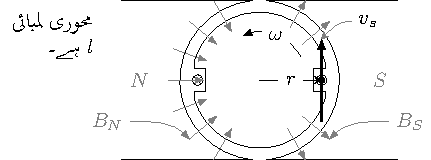
\includegraphics{figRotatingMachPrinciplesSingleTurnProducingEMF}
\begin{tikzpicture}
%grid
%\draw[gray] (-\sRo,-\sRo) grid (\sRo,\sRo);
%ROTOR
\pgfmathsetmacro{\shiftX}{5cm}
\pgfmathsetmacro{\pTheta}{150}
\pgfmathsetmacro{\pY}{0.2}
\rotor{2}{90}
%DOT on rotor
\draw (180:\rR-\pX) circle (2.5pt);
\draw[fill] (180:\rR-\pX) circle (1.5pt);
%CROSS on rotor
\draw (0:\rR-\pX) circle (2.5pt);
\draw (0:\rR-\pX)++(45:2.2pt)--++(-135:4.4pt);
\draw (0:\rR-\pX)++(-45:2.2pt)--++(135:4.4pt);
%STATOR
\draw ([shift={(-85:\sRi+\gap)}]0,0) arc (-85:85:\sRi+\gap);
\draw(85:\sRi+\gap)--++(0:1.2*\sRo);
\draw(-85:\sRi+\gap)--++(0:1.2*\sRo);
\node[very thick] at (0:1.1*\sRo){$S$};
\draw ([shift={(95:\sRi+\gap)}]0,0) arc (95:270-5:\sRi+\gap);
\draw(95:\sRi+\gap)--++(180:1.2*\sRo);
\draw(-95:\sRi+\gap)--++(180:1.2*\sRo);
\node[very thick] at (180:1.1*\sRo){$N$};
%flux at south pole
\foreach \angle in {-60,-40,40,60}{
\draw[-latex] (0,0)++(\angle:\rR-2*\gap)--++(\angle:6*\gap);  }
%
\draw[] (0,0)++(-40:\rR+4*\gap) to [out=45,in=180] ++(1,0.3)node[right]{$B_S$};
%flux at north pole
\foreach \angle in {120,140,160,200,220,240}{
\draw[latex-] (0,0)++(\angle:\rR-2*\gap)--++(\angle:6*\gap);  }
%
\draw[] (0,0)++(220:\rR+4*\gap)++(-0.1,0) to [out=135,in=0] ++(-1,0.3)node[left]{$B_N$};
%velocity
\draw[thick,-latex](0:\rR-\pX)--++(0,-0.7)--++(0,1.4)coordinate (velocityTip);
\draw[] (velocityTip) to [out=45,in=180] ++(0.5,0.3) node[right,text=black] {$v_S$};
%text
\draw[-stealth](0,0)--++(0:\rR-\pX) node[fill=white,pos=0.5]{$r$};
\draw[-latex]([shift={(30:0.7*\rR)}]0,0) arc (30:110:0.7*\rR);
\draw node[fill=white] at (70:0.7*\rR){$\omega$};
%
\draw node[align=right] at (-3.5,0.75){\RL{محوری لمبائی} \\ \RL{$l$ ہے۔}};
\end{tikzpicture}
\caption{ایک چکر کا لچھا مقناطیسی میدان میں گھوم رہا ہے۔}
\label{شکل_گھومتے_مشین_ایک_چکر_کی_پیدا_دباو}
\end{figure}

 حرکت کی مدد سے یوں حاصل برقی دباو کو \اصطلاح{محرک برقی دباو}\فرہنگ{برقی دباو!محرک}\حاشیہب{electromotive force, emf}\فرہنگ{electromotive force}\فرہنگ{emf}  کہتے ہیں۔ روایتی طور پر کسی بھی طریقہ سے حاصل برقی دباو کو محرک برقی دباو کہتے ہیں۔ یوں کیمیائی برقی سیل وغیرہ کا برقی دباو بھی محرک برقی دباو کہلائے  گا۔

شکل \حوالہ{شکل_گھومتے_مشین_ایک_چکر_کی_پیدا_دباو} میں گھڑی کے مخالف رخ گھومتے حصہ پر ایک چکر کا لچھا نسب ہے۔بائیں خلاء میں لچھا کی  تار کے قطع پر غور کریں۔ مساوات \حوالہ{مساوات_گھومتے_مشین_قوت_لورینز}  کے تحت بایاں قطع میں موجود مثبت برقی بار پر صفحہ کے عمودی باہر رخ قوت پیدا ہو گی جبکہ اس قطع میں موجود منفی برقی بار پر اس کے مخالف رخ قوت پیدا ہو گی۔مساوات \حوالہ{مساوات_گھومتے_مشین_برقی_دباو_تعریف}  کے تحت اس قطع کا بالائی  سرا مثبت   اور نچلا سرا منفی برقی دباو پر ہو گا۔

ہم گھومتے حصہ کی محور پر نلکی محدد قائم کرتے ہیں۔ یوں جنوبی قطب کے سامنے خلاء میں \سمتیہ{B} رداسی رخ جبکہ شمالی  قطب کے سامنے  خلاء میں  \سمتیہ{B} رداس کے مخالف رخ ہو گا۔جنوبی قطب کے سامنے شگاف میں برقی تار \سمتیہز{l}{S}  کے لئے ہم درج ذیل لکھ سکتے ہیں۔
\begin{gather}
\begin{aligned}
\kvec{v}_S&=v \atheta =\omega r \atheta\\
\kvec{B}_S&=B \ar\\
\kvec{l}_S&=l \az
\end{aligned}
\end{gather}
یوں  جنوبی قطب کے سامنے تار کے قطع  میں درج ذیل محرک برقی دباو پیدا ہو گا۔
\begin{gather}
\begin{aligned}
e&=(\kvec{v} \times \kvec{B}) \cdot \kvec{l}\\
&=\omega r B l  (\atheta \times \ar) \cdot \az\\
&=\omega r B l  (-\az) \cdot \az\\
&=-\omega r B l 
\end{aligned}
\end{gather}

جنوبی مقناطیسی قطب کے سامنے شگاف میں برقی تار کی لمبائی کا رخ \عددیء{\az} لیا گیا۔اس مساوات میں برقی دباو منفی ہونے کا مطلب ہے کہ برقی تار کا مثبت سرا تار پر \عددیء{-\az} رخ ہے یعنی تار کا نچلا سرا مثبت اور بالائی سرا منفی ہے۔ اگر اس  تار میں  رو گزر سکے تو اس رو کا رخ  \عددیء{-\az} یعنی صفحہ کو عمودی اندر رخ ہو گا جسے  شکل \حوالہ{شکل_گھومتے_مشین_ایک_چکر_کی_پیدا_دباو} میں  شگاف میں دائرہ کے اندر صلیبی نشان سے ظاہر کیا گیا ہے۔ 

اسی طرح شمالی مقناطیسی قطب کے سامنے شگاف میں موجود برقی تار کے لئے ہم درج ذیل لکھ سکتے ہیں۔
\begin{gather}
\begin{aligned}
\kvec{v}_N&=v \atheta=\omega r\atheta\\
\kvec{B}_N&=-B \ar\\
\kvec{l}_N&=l \az
\end{aligned}
\end{gather}
یوں اس قطع میں درج ذیل دباو ہو گا۔
\begin{gather}
\begin{aligned}
e_N&=(\kvec{v}_N \times \kvec{B}_N)\cdot \kvec{l}_N\\
&=-\omega rB l (\atheta \times \ar) \cdot \az\\
&=-\omega r B l (-\az) \cdot \az\\
&=\omega r B l 
\end{aligned}
\end{gather}

شمالی مقناطیسی قطب کے سامنے شگاف میں برقی تار کی لمبائی کا رخ $\az$ لیا گیا ہے۔اس مساوات میں برقی دباو  مثبت ہونے کا مطلب ہے کہ برقی تار کا مثبت سرا تار پر  $\az$ رخ ہو گا یعنی تار کا بالائی سرا مثبت اور نچلا  سرا منفی ہو گا۔اگر اس تار میں  رو گزر سکے تو اس کا رخ $\az$ یعنی صفحہ کو عمودی  باہر رخ ہو گا جسے شکل \حوالہ{شکل_گھومتے_مشین_ایک_چکر_کی_پیدا_دباو} میں  شگاف میں دائرہ کے اندر نقطہ کے نشان سے دکھایا گیا ہے۔ 

یہ دونوں  تار مل کر ایک چکر کا لچھا بناتے ہیں۔ ان تاروں  کے نچلے سر ایک دوسرے کے ساتھ سلسلہ وار جڑے ہیں جس کو شکل میں نہیں دکھایا گیا۔یوں اس لچھے کے بالائی،  نظر آنے والے،  سروں پر کل برقی دباو \عددیء{e} ان دو برقی تاروں میں پیدا برقی دباو  کا مجموعہ ہو گا:
\begin{gather}
\begin{aligned}
e&=2r l B \omega\\
&=A B \omega
\end{aligned}
\end{gather}
یہاں لچھے کا رقبہ  \عددیء{A=2 r l } ہے۔اگر ایک چکر سے اتنا برقی دباو حاصل ہو تب \عددیء{N} چکر کے لچھے  سے درج ذیل دباو حاصل ہو گا جہاں \عددی{\phi=AB} مقناطیسی بہاو ہے۔
\begin{gather}
\begin{aligned}\label{مساوات_گھومتے_مشین_پیدا_دباو}
e&=\omega N A B\\
&=2 \pi f N A B\\
&=2 \pi f N \phi
\end{aligned}
\end{gather}

گھومتی مشینوں کی خلائی درز میں  \سمتیہ{B} اور \سمتیہ{v}  ہر لمحہ ایک دوسرے کے عمودی ہوتے ہیں۔مساوات \حوالہ{مساوات_گھومتے_مشین_برقی_دباو_تعریف}  کے تحت مستقل زاویائی  رفتار اور محوری لمبائی کی صورت میں پیدا کردہ برقی دباو  ہر لمحہ  \عددیء{B} کا براہ راست متناسب ہو گا۔ خلائی درز میں زاویہ کے ساتھ  تبدیل ہوتے ہوئے \عددیء{B} کی صورت میں گھومتے لچھے میں پیدا برقی دباو بھی زاویہ کے ساتھ تبدیل ہو گا۔یوں جس شکل کا برقی دباو درکار ہو اسی شکل کی کثافت مقناطیسی دباو خلائی درز میں پیدا کرنی ہو گی۔سائن نما برقی دباو پیدا کرنے کے لئے   خلائی درز میں  سائن نما کثافتِ مقناطیسی بہاو درکار ہو گی۔

اگلے حصے میں خلائی درز میں ضرورت کے تحت \عددیء{B}  پیدا کرنے کی ترکیب بتلائی جائے گی۔

\حصہ{پھیلے لچھے  اور سائن نما مقناطیسی دباو}
ہم نے اب تک جتنے مشین دیکھے ان سب میں گچھ\حاشیہب{non-distributed coils} لچھے دکھائے گئے۔ مزید  ان مشینوں میں گھومتے حصے پر موجود مقناطیس کے \اصطلاح{ابھرے قطب}\فرہنگ{قطب!ابھرے}\حاشیہب{salient poles}\فرہنگ{pole!salient} تھے۔ عموماً حقیقی مشینوں کے  \اصطلاح{ہموار قطب}\فرہنگ{قطب!ہموار}\حاشیہب{non-salient poles}\فرہنگ{pole!non-salient} اور \اصطلاح{پھیلے لچھے}\فرہنگ{لچھا!پھیلے}\حاشیہب{distributed winding}\فرہنگ{winding!distributed} ہوتے ہیں جن کی بنا ساکن اور گھومتے حصوں کے بیچ  خلائی درز میں سائن نما مقناطیسی دباو اور سائن نما  کثافت مقناطیسی بہاو پیدا کرنا ممکن ہوتا ہے۔ 
\begin{figure}
\centering
%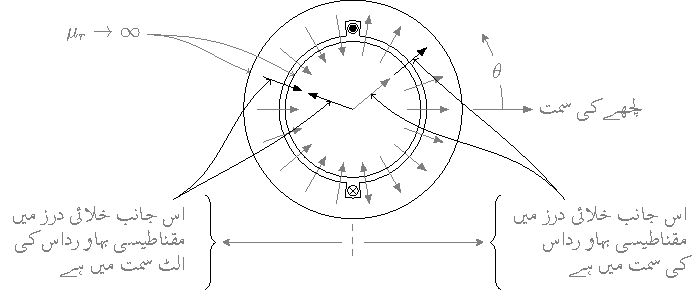
\includegraphics{figRotatingMachPrinciplesStatorCoilNotDistributed}
\begin{tikzpicture}
\stator{2}{90}
\slotDot{90}
\slotCross{270}
\draw (0,0) circle (\rR);
%FLUX
\foreach \angle in {-80,-60,-40,-20,0,20,40,60,80}{
\draw[-latex] (\angle:0.8*\rR) --++(\angle:0.7); }
\foreach \angle in {100,120,140,160,180,200,220,240,260,280}{
\draw[latex-] (\angle:0.8*\rR) --++(\angle:0.7); }
%text
\draw[-latex] (0:1.1*\sRo)--++(0:1)node[right] {\RL{لچھے کا رخ}};
\draw[-stealth]([shift={(0:1.1*\sRo+0.5)}]0,0) arc (0:30:1.1*\sRo+0.5);
\draw node[fill=white] at (15:1.1*\sRo+0.5){$\theta$};
\draw[dashed] (-90:\sRo+0.1)--++(0,-0.6);
%radial direction and flux
\draw[-latex] (0,0) --(40:0.7*\rR)coordinate[pos=0.5](kradial);
\draw[-latex] (0,0) --(160:0.7*\rR)coordinate[pos=0.5](kradialO);
\draw[-latex] (40:0.8*\rR) --++(40:0.7)coordinate[pos=0.6](kflux); 
\draw[latex-] (160:0.8*\rR) --++(160:0.7)coordinate[pos=0.8](kfluxO); 
%text
\draw[-stealth] (-90:\sRo+0.4)++(0.2,0) --++(2,0)node[xshift=0.4cm,right,align=right](kNOTopposing){\RL{اس جانب خلائی درز میں} \\ \RL{مقناطیسی بہاو رداسی} \\ \RL{رخ ہے۔}};
\draw[-stealth] (-90:\sRo+0.4)++(-0.2,0) --++(-2,0)node[xshift=-0.5cm,left,align=right](kOpposing){\RL{اس جانب خلائی درز میں} \\ \RL{مقناطیسی بہاو رداسی} \\ \RL{رخ کے مخالف ہے۔}};
\draw[<-](kradial) to [out=-45,in=130] (kNOTopposing);
\draw[<-](kflux) to [out=-45,in=130] (kNOTopposing);
\draw[<-](kradialO) to [out=220,in=30] (kOpposing);
\draw[<-](kfluxO) to [out=220,in=30] (kOpposing);
\draw node[left] at (160:2*\sRo)(kmu){$\mu_r \to \infty$};
\draw[<-] (160:\sRo) to [out=160,in=0] (kmu);
\draw[<-] (150:\rR) to [out=150,in=0] (kmu);
%brace
\draw[decorate,decoration={brace,amplitude=5pt}] (-90:\sRo+0.4)++(-0.5,0) ++(-2,0)++(0,0.8) -- ++(0,-1.6) node [black,midway,xshift=9pt] {};
\draw[decorate,decoration={brace,amplitude=5pt}] (-90:\sRo+0.4)++(0.5,0) ++(2,0)++(0,-0.8) -- ++(0,1.6) node [black,midway,xshift=9pt] {};
\end{tikzpicture}
\caption{ساکن لچھا گچھ ہے۔}
\label{شکل_گھومتے_مشین_گچھ_لچھا}
\end{figure}

شکل \حوالہ{شکل_گھومتے_مشین_گچھ_لچھا}  میں ایک  گچھ لچھا  دکھایا گیا ہے جہاں مشین کے گھومتے حصے کا عمودی تراش گول صورت کا  ہے۔ متحرک اور ساکن  قالب  کا \عددیء{\mu_r \to \infty} ہے۔لچھے کا مقناطیسی دباو \عددیء{\tau=N i}،  مقناطیسی بہاو \عددیء{\phi} پیدا کرتا  ہے جس کو ہلکی سیاہی کی  لکیروں سے ظاہر کیا گیا ہے۔ مقناطیسی بہاو خلائی درز میں سے دو مرتبہ گزرتا ہوا لچھے کے گرد ایک چکر کاٹتا ہے لہٰذا  درج ذیل ہو گا۔
\begin{align}
\tau=N i=2 H l_a
\end{align}
%
\begin{figure}
\centering
%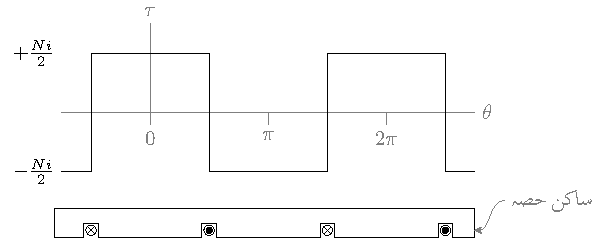
\includegraphics{figRotatingMachPrinciplesMMFjumpsAtDotAndCross}
\begin{tikzpicture}
\begin{scope}[yshift=-2cm]
\dotLinear{1,5}
\crossLinear{-1,3}
\slotSegment{-1/1,1/3,3/5}
\slotTop{-1/5}
\draw[stealth-] (5.5,0) to [out=0,in=180] (6,0.5)node[right]{\RL{ساکن حصہ}};
\end{scope}
%
\draw[](-1.5,0)--(5.5,0)node[right]{$\theta$};
\draw[](0,0)--(0,1.5)node[above]{$\tau$};
\foreach \x/\labelText in {0/0,2/\pi,4/2\pi}{
\draw[](\x,0)--++(0,-0.2) node[below]{$\labelText$};}
\draw(-1.5,-1)--(-1,-1)--(-1,1)--(1,1)--(1,-1)--(3,-1)--(3,1)--(5,1)--(5,-1)--(5.5,-1);
%text
\draw node[left] at (-1.5,1){$+\tfrac{Ni}{2}$};
\draw node[left] at (-1.5,-1){$-\tfrac{Ni}{2}$};
\end{tikzpicture}
\caption{گچھ لچھے کی خلائی درز میں مقناطیسی دباو۔}
\label{شکل_گھومتے_مشین_گچھ_لچھے_کا_دباو}
\end{figure}

یوں ساکن لچھے کے مقناطیسی دباو  کا  آدھا حصہ  ایک خلائی درز اور آدھا حصہ  دوسرے خلائی درز میں مقناطیسی بہاو پیدا کرتا ہے۔ مزید  آدھے خلائی درز میں مقناطیسی دباو ( اور  مقناطیسی بہاو )  رداسی رخ  اور باقی خلائی درز میں  رداس کے مخالف رخ ہے۔ ہم رداسی رخ  کو مثبت تصور کرتے ہیں۔ چونکہ مقناطیسی بہاو ( اور مقناطیسی دباو ) \عددیء{-\tfrac{\pi}{2} < \theta< \tfrac{\pi}{2}} کے درمیان رداسی رخ ہے لہٰذا اسے مثبت تصور کیا جائے گا جبکہ باقی حصہ پر مقناطیسی دباو ( اور مقناطیسی بہاو ) رداس کے مخالف رخ ہے لہٰذا  اسے منفی تصور کیا جائے گا۔  شکل \حوالہ{شکل_گھومتے_مشین_گچھ_لچھے_کا_دباو} میں خلائی درز میں مقناطیسی دباو کو زاویہ کے ساتھ ترسیم کیا گیا ہے۔ وقفہ \عددیء{-\tfrac{\pi}{2} < \theta <\tfrac{\pi}{2}} کے خلائی درز میں مقناطیسی دباو \عددیء{\tau_a} لچھے کے مقناطیسی دباو \عددیء{\tau} کا آدھا ہے اور اس کا رخ مثبت ہے جبکہ وقفہ \عددیء{\tfrac{\pi}{2} < \theta <\tfrac{3 \pi}{2}} کے خلائی درز میں مقناطیسی دباو لچھے کے مقناطیسی دباو کا آدھا  اور منفی رخ  ہے۔ یاد رہے مقناطیسی دباو کا رخ\فرہنگ{مقناطیسی دباو!رخ}  رداسی رخ کے حوالہ  سے تعین کیا جاتا ہے۔

\جزوحصہ{بدلتا رو والے مشین}
بدلتا رو (اے سی) مشین بناتے وقت  کوشش کی جاتی ہے کہ خلائی درز میں مقناطیسی دباو سائن نما ہو۔سائن نما مقناطیسی دباو کے حصول  کی خاطر لچھوں کو ایک سے زیادہ شگافوں میں تقسیم کیا جاتا ہے۔ ایسا کرنے سے سائن نما مقناطیسی دباو کیسے حاصل ہوتا ہے، اس بات کی  یہاں وضاحت کی جائے گی۔

\اصطلاح{فوریئر} تسلسل\فرہنگ{فوریئر تسلسل}\حاشیہب{Fourier series}\فرہنگ{Fourier series} کے تحت ہم کسی بھی تفاعل\حاشیہب{function} \عددیء{f(\theta_p)}  کو درج ذیل صورت میں لکھ سکتے ہیں۔
\begin{align}
f(\theta_p)=\sum_{n=0}^{\infty} (a_n \cos n \theta_p +b_n \sin n \theta_p)
\end{align}
تفاعل کا دوری عرصہ\فرہنگ{دوری عرصہ}\حاشیہب{time period}\فرہنگ{time period} \عددیء{T} ہونے کی صورت میں فوریئر تسلسل کے عددی سر درج ذیل ہوں گے۔
\begin{gather}
\begin{aligned}\label{مساوات_گھومتے_مشین_فورئر_تسلسل_جزو}
a_0&=\frac{1}{T} \int_{-T/2}^{T/2} f(\theta_p) \dif \theta_p\\
a_n&=\frac{2}{T} \int_{-T/2}^{T/2} f(\theta_p) \cos n \theta_p \dif \theta_p\\
b_n&=\frac{2}{T} \int_{-T/2}^{T/2} f(\theta_p) \sin n \theta_p \dif \theta_p
\end{aligned}
\end{gather}
%
\ابتدا{مثال}\شناخت{مثال_تبادلہ_توانائی_فوریئر_تسلسل}
شکل \حوالہ{شکل_گھومتے_مشین_گچھ_لچھے_کا_دباو}  میں دیے گئے مقناطیسی دباو کا
\begin{itemize}
\item
فوریئر تسلسل حاصل کریں،
\item
تیسری موسیقائی جزو\فرہنگ{موسیقائی جزو}\حاشیہب{third harmonic component}\فرہنگ{harmonic} اور بنیادی جزو\فرہنگ{بنیادی جزو}\حاشیہب{fundamental component}\فرہنگ{fundamental} کا تناسب معلوم کریں۔
\end{itemize}

حل:
\begin{itemize}
\item
مساوات \حوالہ{مساوات_گھومتے_مشین_فورئر_تسلسل_جزو}  کی مدد سے

\begin{align*}
a_0&=\frac{1}{2\pi} \left[\int_{-\pi}^{-\pi/2} \left(-\frac{Ni}{2} \right) \dif \theta_p+\int_{-\pi/2}^{\pi/2} \left (\frac{Ni}{2}\right) \dif \theta_p +\int_{\pi/2}^{\pi} \left(-\frac{Ni}{2}\right) \dif \theta_p  \right]\\
&=\frac{1}{2\pi} \left[\left(-\frac{Ni}{2} \right)\left(-\frac{\pi}{2}+\pi \right) +\left(\frac{Ni}{2} \right)\left(\frac{\pi}{2}+\frac{\pi}{2} \right)+\left(-\frac{Ni}{2} \right)\left(\pi-\frac{\pi}{2} \right)\right]\\
&=0
\end{align*}
اور درج ذیل حاصل ہوں گے۔
\begin{align*}
a_n&=\frac{2}{2\pi} \frac{Ni}{2} \left[\int_{-\pi}^{-\pi/2} -\cos n \theta_p \dif \theta_p +\int_{-\pi/2}^{\pi/2} \cos n \theta_p \dif \theta_p+\int_{\pi/2}^{\pi} -\cos n \theta_p \dif \theta_p\right]\\
&=\frac{Ni}{2\pi} \left[-\left. \frac{\sin n \theta_p}{n}\right|_{-\pi}^{-\pi/2} +\left. \frac{\sin n \theta_p}{n}\right|_{-\pi/2}^{\pi/2} -\left. \frac{\sin n \theta_p}{n}\right|_{\pi/2}^{\pi} \right]\\
&=\frac{Ni}{2n\pi} \left[\sin \frac{n\pi}{2}+2\sin \frac{n\pi}{2}+\sin \frac{n\pi}{2} \right]\\
&=\left(\frac{4}{n\pi}\right) \left( \frac{Ni}{2}\right) \sin \frac{n\pi}{2}
\end{align*}
اس مساوات میں \عددیء{n} کی قیمت ایک، دو، تین لیتے ہوئے درج ذیل حاصل ہوتا ہے۔
\begin{align*}
a_1&=\left(\frac{4}{\pi}\right) \left( \frac{Ni}{2}\right), \quad a_3=-\left(\frac{4}{3\pi}\right) \left( \frac{Ni}{2}\right), \quad a_5=\left(\frac{4}{5\pi}\right) \left( \frac{Ni}{2}\right)\\
a_2&=a_4=a_6=0
\end{align*}
اسی طرح درج ذیل ہو گا۔
\begin{align*}
b_n&=\frac{2}{2\pi} \frac{Ni}{2} \left[\int_{-\pi}^{-\pi/2} -\sin n \theta_p \dif \theta_p +\int_{-\pi/2}^{\pi/2} \sin n \theta_p \dif \theta_p+\int_{\pi/2}^{\pi} -\sin n \theta_p \dif \theta_p\right]\\
&=\frac{Ni}{2\pi} \left[\left. \frac{\cos n \theta_p}{n}\right|_{-\pi}^{-\pi/2} -\left. \frac{\cos n \theta_p}{n}\right|_{-\pi/2}^{\pi/2} +\left. \frac{\cos n \theta_p}{n}\right|_{\pi/2}^{\pi} \right]\\
&=0
\end{align*}
\item
ان نتائج کا یکجا کرتے ہیں:
\begin{align*}
\abs{\frac{a_3}{a_1}} =\frac{\left(\frac{4}{3\pi}\right) \left( \frac{Ni}{2}\right)}{\left(\frac{4}{\pi}\right) \left( \frac{Ni}{2}\right)}=\frac{1}{3}
\end{align*}
\end{itemize}
یوں تیسرا موسیقائی جزو بنیادی جزو کا تیسرا حصہ یعنی \عددیء{33.33} فی صد ہو گا۔
\انتہا{مثال}
%
مثال \حوالہ{مثال_تبادلہ_توانائی_فوریئر_تسلسل} میں حاصل کردہ  \عددیء{a_1,a_2,\cdots} استعمال کرتے ہوئے  ہم خلائی درز میں مقناطیسی دباو \عددیء{\tau} کا فوریئر تسلسل لکھتے ہیں۔
\begin{align}\label{مساوات_تبادلہ_توانائی_فوریئر_متقناطیسی_دباو_تسلسل}
\tau_a=\frac{4}{\pi}\frac{Ni}{2} \cos \theta_p-\frac{4}{3\pi}\frac{Ni}{2} \cos 3\theta_p+\frac{4}{5\pi}\frac{Ni}{2} \cos 5\theta_p+\cdots
\end{align}
مثال \حوالہ{مثال_تبادلہ_توانائی_فوریئر_تسلسل} کے مقناطیسی دباو کے موسیقائی اجزاء  کی قیمتیں اتنی کم نہیں کہ انہیں رد کیا جا سکے۔جیسا آپ اس باب میں آگے دیکھیں گے حقیقی  مقناطیسی دباو کے موسیقائی اجزاء قابل نظر انداز ہوں گے اور ہمیں صرف بنیادی جزو  سے غرض ہو گا۔اسی حقیقت کو مد نظر رکھتے ہوئے ہم  تسلسل کے موسیقائی اجزاء کو نظر انداز کرتے ہوئے  مساوات \حوالہ{مساوات_تبادلہ_توانائی_فوریئر_متقناطیسی_دباو_تسلسل} سے
\begin{align}\label{مساوات_گھومتے_مشین_پھیلا_سائن_نما}
\tau_{a}=\frac{4}{\pi}\frac{Ni}{2} \cos \theta_p=\tau_0 \cos \theta_p
\end{align}
لکھتے ہیں جہاں \عددی{\tau_0} درج ذیل ہے۔
\begin{align}\label{مساوات_گھومتے_مشین_دباو_چوٹی}
\tau_0=\frac{4}{\pi}\frac{Ni}{2} 
\end{align}

خلائی درج میں \عددی{\tau}، \عددی{H} اور \عددی{B} ایک دوسرے کے برائے راست متناسب ہوتے ہیں۔ یوں 
مساوات \حوالہ{مساوات_گھومتے_مشین_پھیلا_سائن_نما} کے تحت  شکل \حوالہ{شکل_گھومتے_مشین_گچھ_لچھا}  کا لچھے اور  شکل \حوالہ{شکل_گھومتے_مشین_رداس_اور_مقناطیسی_بہاو}  میں  صفر زاویہ پر سلاخ نما مقناطیس یکساں \عددی{\tau} (اور \عددی{B}) دیں گے۔ اسی طرح اگر شکل \حوالہ{شکل_گھومتے_مشین_گچھ_لچھا}  کا لچھا  زاویہ \عددیء{\theta_m}  پر  ہوتا تب ہمیں  شکل \حوالہ{شکل_گھومتے_مشین_رداس_اور_مقناطیسی_بہاو_مقناطیس_گھوما_ہے}  میں موجود مقناطیس کے نتائج حاصل ہوتے۔

 شکل \حوالہ{شکل_گھومتے_مشین_تین_دور_لچھے}  میں تین لچھے آپس میں \عددی{120\degree} زاویہ پر دکھائے گئے ہیں۔ ہم مساوات \حوالہ{مساوات_گھومتے_مشین_کثافت_بالمقابل_زاویہ}   کی طرح اس شکل میں لچھا  \عددیء{a} کے لئے درج ذیل لکھ سکتے ہیں۔
\begin{figure}
\centering
%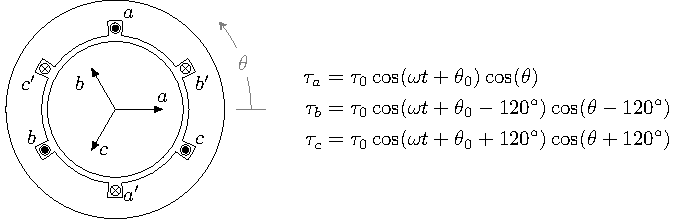
\includegraphics{figRotatingMachPrinciplesThreePhaseSynchronousMachine}
\begin{tikzpicture}
\stator{6}{30}
\slotDot{90,210,330}
\slotCross{30,150,270}
%\slotName{comma separated angles/name/NameAtleftORrightOfSlot}
\slotName{90/a/above right,210/b/above left,330/c/above right}
\slotName{30/b'/below right,150/c'/below left,270/a'/right}
%
\draw (0,0) circle (\rR);
\draw[-latex] (0,0)--++(0:0.7*\rR)node [above]{$a$};
\draw[-latex] (0,0)--++(120:0.7*\rR)node [below left]{$b$};
\draw[-latex] (0,0)--++(-120:0.7*\rR)node [right]{$c$};
%
\draw[](0:\sRo+0.2)--++(0:0.5 )coordinate[pos=0.5] (angleZero);
\draw[-stealth](angleZero) arc (0:40:\sRo+0.2+0.25);
\draw node[fill=white] at (20:\sRo+0.2+0.25){$\theta$};
\end{tikzpicture}
\caption{تین دور لچھے۔}
\label{شکل_گھومتے_مشین_تین_دور_لچھے}
\end{figure}
%
\begin{gather}
\begin{aligned}\label{مساوات_گھومتے_مشین_الف_موج}
\tau_a&=\tau_0 \cos \theta_{p_a}\\
\theta_{p_a}&=\theta-\theta_{m_a}=\theta-0\degree\\
\tau_a&=\tau_0 \cos (\theta-\theta_m)=\tau_0 \cos \theta
\end{aligned}
\end{gather}
اسی طرح لچھا \عددیء{b} اور \عددیء{c} جو بالترتیب \عددیء{\theta_{m_b}=120\degree} اور \عددیء{\theta_{m_c}=240\degree}  زاویہ پر ہیں کے لئے درج ذیل ہو گا۔
\begin{gather}
\begin{aligned}\label{مساوات_گھومتے_مشین_ب_موج}
\tau_b&=\tau_0 \cos \theta_{p_b}\\
\theta_{p_b}&=\theta-\theta_{m_b}=\theta-120\degree\\
\tau_b&=\tau_0 \cos (\theta-\theta_{m_b})=\tau_0 \cos (\theta-120\degree)
\end{aligned}
\end{gather}
%
\begin{gather}
\begin{aligned}\label{مساوات_گھومتے_مشین_پ_موج}
\tau_c&=\tau_0 \cos \theta_{p_c}\\
\theta_{p_c}&=\theta-\theta_{m_c}=\theta-240\degree\\
\tau_c&=\tau_0 \cos (\theta-\theta_{m_c})=\tau_0 \cos (\theta-240\degree)=\tau_0 \cos (\theta+120\degree)
\end{aligned}
\end{gather}

اگرچہ ظاہری طور پر خلائی درز میں مقناطیسی دباو سائن نما ہرگز نہیں لگتا لیکن مساوات \حوالہ{مساوات_تبادلہ_توانائی_فوریئر_متقناطیسی_دباو_تسلسل}  ہمیں بتلاتی ہے کہ یہ محض نظر کا دھوکا ہے۔ اس مقناطیسی دباو کا بیشتر حصہ سائن نما ہی ہے۔  اگر ہم کسی طرح مساوات \حوالہ{مساوات_تبادلہ_توانائی_فوریئر_متقناطیسی_دباو_تسلسل}   میں پہلے رکن کے علاوہ باقی تمام ارکان کو صفر کر سکیں تب ہمیں   سائن نما مقناطیسی دباو حاصل ہو گا۔

\begin{figure}
\centering
%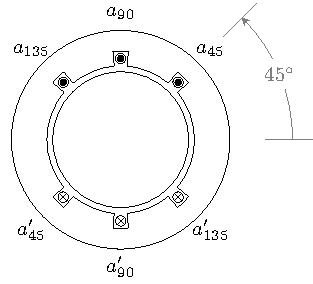
\includegraphics{figRotatingMachPrinciplesDistributedStatorWinding}
\begin{tikzpicture}
%grid
%\draw[gray] (-\sRo,-\sRo) grid (\sRo,\sRo);
%
\statorEach{45/90,90/135,135/225,225/270,270/315,315/405}
\draw (0,0) circle (\rR);
\slotDot{45,90,135}
\slotCross{-45,-90,-135}
\draw node at (45:\sRo+0.3) {$a_{45}$};
\draw node at (90:\sRo+0.3) {$a_{90}$};
\draw node at (135:\sRo+0.3) {$a_{135}$};
\draw node at (225:\sRo+0.3) {$a_{45}'$};
\draw node at (270:\sRo+0.3) {$a_{90}'$};
\draw node at (315:\sRo+0.3) {$a_{135}'$};
%text
\draw[] (0:\sRo+0.6)--++(0:0.7*\rR);
\draw[](45:\sRo+0.6)--++(45:0.7*\rR);
\draw[-stealth] (0:\sRo+0.6+0.4*\rR) arc (0:45:\sRo+0.6+0.4*\rR);
\draw node[fill=white] at (22.5:\sRo+0.6+0.4*\rR){$45\degree$};
\end{tikzpicture}%
\caption{پھیلا لچھا۔}
\label{شکل_گھومتے_مشین_پھیلا_لچھا}
\end{figure}

شکل \حوالہ{شکل_گھومتے_مشین_گچھ_لچھا} کے \عددیء{N} چکر  لچھے کو تین چھوٹے یکساں لچھوں میں تقسیم  کرتے ہوئے شکل \حوالہ{شکل_گھومتے_مشین_پھیلا_لچھا}  حاصل کیا گیا ہے جہاں ہر چھوٹا لچھا \عددیء{\tfrac{N}{3}} چکر کا ہے۔  ایسے چھوٹے لچھوں کو سلسلہ وار جوڑا\فرہنگ{سلسلہ وار}\حاشیہب{series connected} جاتا ہے لہٰذا ان میں ایک جیسا  برقی رو \عددیء{i} گزرے گا۔ ان تین لچھوں کو تین مختلف شگافوں میں رکھا گیا ہے۔پہلے لچھے کو شگاف \عددیء{a_{45}} اور \عددیء{a_{45}'} میں رکھا گیا ہے۔ دوسرے لچھے کو شگاف \عددیء{a_{90}} اور \عددیء{a_{90}'} میں اور تیسرے لچھے کو شگاف \عددیء{a_{135}} اور \عددیء{a_{135}'} میں رکھا گیا ہے۔
\begin{figure}
\centering
%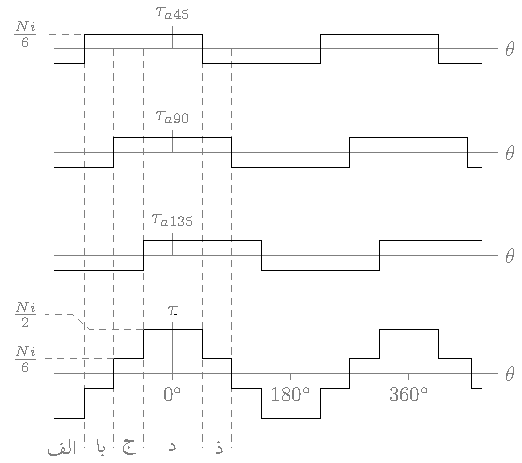
\includegraphics{figRotatingMachPrinciplesMMFjumpsThreePhase}
\begin{tikzpicture}
%
\pgfmathsetmacro{\j}{0.25}
\pgfmathsetmacro{\shiftY}{0.35}
%
%dashed vertical lines
\draw[dashed](-135/90,0)--(-135/90,-12*\shiftY-5*\j)node[left]{\textup{ا}};
\draw[dashed](-90/90,-3.5*\shiftY)--(-90/90,-12*\shiftY-5*\j)node[left]{\textup{ب}};
\draw[dashed](-45/90,-7*\shiftY)--(-45/90,-12*\shiftY-5*\j)node[left]{\textup{ج}};
\draw[dashed](45/90,0)--(45/90,-12*\shiftY-5*\j)node[xshift=-0.5 cm]{\textup{د}};
\draw[dashed](90/90,-3.5*\shiftY)--(90/90,-12*\shiftY-5*\j)node[left]{\textup{ذ}};
%axis
\draw[](-2,0)--(5.5,0)node[right]{$\theta$};
\draw[](0,0)--(0,2*\j)node[above]{$\tau_{a45}$};
%\draw (-45/90,0)--++(0,-0.2)node[below,gray]{$-45\degree$};
%
\mmf{-180/-\j/-135/\j,-135/\j/45/-\j,45/-\j/225/\j,225/\j/405/-\j}
\draw(405/90,-\j)--(470/90,-\j);
%text
\draw[dashed]  (-140/90,\j)--++(-0.6,0)node[left,solid]{$\tfrac{N i}{6}$};
%
\begin{scope}[yshift=-3.5*\shiftY cm]
%axis
\draw[](-2,0)--(5.5,0)node[right]{$\theta$};
\draw[](0,0)--(0,2*\j)node[above]{$\tau_{a90}$};;
%
\mmf{-180/-\j/-90/\j,-90/\j/90/-\j,90/-\j/270/\j,270/\j/450/-\j}
\draw(450/90,-\j)--(470/90,-\j);
\end{scope}
%
\begin{scope}[yshift=-7*\shiftY cm]
%axis
\draw[](-2,0)--(5.5,0)node[right]{$\theta$};
\draw[](0,0)--(0,2*\j)node[above]{$\tau_{a135}$};
%\draw(45/90,0)--++(0,-0.2)node[below,gray]{$45\degree$};
%
\mmf{-180/-\j/-45/\j,-45/\j/135/-\j,135/-\j/315/\j}
\draw(315/90,\j)--(470/90,\j);
\end{scope}
%
\begin{scope}[yshift=-12*\shiftY cm,xscale=1/90]   %,xscale=1/3 cm
%axis
\draw[](-2*90,0)--(5.5*90,0)node[right]{$\theta$};
\draw[](0,0)--(0,4*\j)node[above]{$\tau$};
\draw[] (0,0)--++(0,-0.1)node[below]{$0\degree$};
\draw[] (180,0)--++(0,-0.1)node[below]{$180\degree$};
\draw[] (360,0)--++(0,-0.1)node[below]{$360\degree$};
%
\draw[thick](-180,-3*\j)--(-135,-3*\j)--(-135,-\j)--(-90,-\j)--(-90,\j)--(-45,\j)--(-45,3*\j)--(45,3*\j)--(45,\j)--(90,\j)--(90,-\j)--(135,-\j)--(135,-3*\j)--(225,-3*\j)--(225,-\j)--(270,-\j)--(270,\j)--(315,\j)--(316,3*\j)--(405,3*\j)--(405,\j)--(455,\j)--(455,-\j)--(470,-\j);
%text
\draw[dashed]  (-90,\j)--(-140-0.6*90,\j)node[left,solid]{$\tfrac{N i}{6}$};
\draw[dashed]  (-45,3*\j)--++(-0.9*90,0)--++(-0.3*90,\j)--(-140-0.6*90,4*\j)node[left,solid]{$\tfrac{N i}{2}$};
\end{scope}
\end{tikzpicture}
\caption{پھیلے لچھے کا کل مقناطیسی دباو۔}
\label{شکل_گھومتے_مشین_پھیلے_لچھے_کی_دباو}
\end{figure}


شگافوں کے ایک جوڑا کو ایک ہی طرح کے نام دیے گئے ہیں، البتہ ایک شگاف کو \عددیء{a} اور دوسرے کو \عددیء{a'} نام دیا گیا ہے۔یوں شگافوں کا پہلے جوڑا  \عددیء{a_{45}} اور \عددیء{a_{45}'}  ہے۔ شگاف   کا نام شگاف کے زاویہ کے لحاظ سے رکھا گیا ہے۔یوں  شگاف  \عددیء{a_{45}} درحقیقت \عددیء{45\degree} زاویہ پر ہے، شگاف \عددیء{a_{90}} نوے درجہ زاویہ پر اور شگاف \عددیء{a_{135}}  ایک سو پینتیس درجہ زاویہ پر ہے۔اسی طرح  \عددی{a'_{45}} شگاف \عددی{a_{45}} کا جوڑا ہے۔

تمام لچھے \عددیء{\tfrac{N}{3}} چکر کے ہیں اور تمام لچھوں میں  برقی رو \عددیء{i} ایک دوسرے جیسا ہے۔  شکل \حوالہ{شکل_گھومتے_مشین_پھیلا_لچھا}   کے  پھیلے لچھے کا مقناطیسی دباو بالمقابل زاویہ کا ترسیم شکل \حوالہ{شکل_گھومتے_مشین_پھیلے_لچھے_کی_دباو}  میں موٹی لکیر سے دکھایا گیا ہے۔سب سے اوپر لچھا  \عددیء{a_{45}}  کے مقناطیسی دباو کی ترسیم ہے جو  شکل \حوالہ{شکل_گھومتے_مشین_گچھ_لچھے_کا_دباو}  کی ترسیم کی طرح لیکن صفر زاویہ سے \عددیء{-45\degree} ہٹ کر ہے۔دوسری ترسیم لچھا \عددیء{a_{90}} کی ہے جو ہو بہو شکل \حوالہ{شکل_گھومتے_مشین_گچھ_لچھے_کا_دباو}   کی طرح ہے جبکہ تیسری ترسیم  لچھا \عددیء{a_{135}} کی ہے جو صفر زاویہ سے \عددیء{+45\degree} ہٹ کر ہے۔ان تینوں ترسیمات کا انفرادی طول \عددیء{\tfrac{Ni}{6}} ہے۔


ترسیمات \عددی{\tau_{a45}}، \عددی{\tau_{a90}} اور \عددی{\tau_{a135}} سے کل مقناطیسی دباو کی ترسیم \عددی{\tau}  حاصل کرنا سیکھتے ہیں۔شکل \حوالہ{شکل_گھومتے_مشین_پھیلے_لچھے_کی_دباو} میں عمودی نقطہ دار لکیریں لگائی گئی ہیں۔ سب سے بائیں  پہلی لکیر کی بائیں طرف خطہ کو "ا" کہا گیا ہے۔اس خطہ میں ترسیمات \عددی{\tau_{a45}}، \عددی{\tau_{a90}} اور \عددی{\tau_{a135}} کی انفرادی قیمتیں \عددیء{-\tfrac{Ni}{6}} ہیں لہٰذا ان کا مجموعہ \عددیء{-\tfrac{Ni}{2}} ہو گا۔یوں خطہ "ا" میں  کل مقناطیسی دباو \عددی{\tau}  کی ترسیم کی قیمت \عددیء{-\tfrac{Ni}{2}}  ہو گی۔ اسی طرح خطہ "ب" میں \عددی{\tau_{a45}} کی قیمت \عددیء{+\tfrac{Ni}{6}} ، \عددی{\tau_{a90}} کی \عددیء{-\tfrac{Ni}{6}} اور \عددی{\tau_{a135}} کی بھی \عددیء{-\tfrac{Ni}{6}} ہے۔ ان کا مجموعہ \عددیء{-\tfrac{Ni}{6}}  ہے جو کل مقناطیسی دباو \عددی{\tau} ہو گا۔خطہ "ج" میں  بالائی تینوں ترسیمات کی قیمتیں بالترتیب  \عددیء{+\tfrac{Ni}{6}}، \عددیء{+\tfrac{Ni}{6}} اور \عددیء{-\tfrac{Ni}{6}}  ہیں جن کا مجموعہ \عددیء{+\tfrac{Ni}{6}}  کل مقناطیسی دباو ہو گا۔ اسی طرح آپ پوری ترسیم کھینچ سکتے ہیں۔

\begin{figure}
\centering
%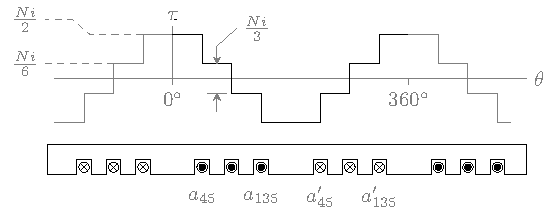
\includegraphics{figRotatingMachPrinciplesDistributedWindingDotAndCross}
\begin{tikzpicture}
\pgfmathsetmacro{\j}{0.25}
\pgfmathsetmacro{\shiftY}{-1.5 cm}
\begin{scope}[xscale=1/90]   %,xscale=1/3 cm
%axis
\draw[](-2*90,0)--(6*90,0)node[right]{$\theta$};
\draw[](0,0)--(0,3.5*\j)node[above]{$\tau$};
%
\draw[](-180,-3*\j)--(-135,-3*\j)--(-135,-\j)--(-90,-\j)--(-90,\j)--(-45,\j)--(-45,3*\j)--(0,3*\j);
\draw[thick] (0,3*\j)--(45,3*\j)--(45,\j)--(90,\j)--(90,-\j)--(135,-\j)--(135,-3*\j)--(225,-3*\j)--(225,-\j)--(270,-\j)--(270,\j)--(315,\j)--(315,3*\j)--(360,3*\j);
\draw[] (360,3*\j)--(405,3*\j)--(405,\j)--(450,\j)--(450,-\j)--(495,-\j)--(495,-3*\j)--(515,-3*\j);
\draw(315/90,1)--(470/90,1);
%text
\draw[] (0,0)--(0,-0.1)node[,below]{$0\degree$};
\draw[] (360,0)--(360,-0.1)node[below]{$360\degree$};
\draw[dashed]  (-90,\j)--(-140-0.6*90,\j)node[left,solid]{$\tfrac{N i}{6}$};
\draw[dashed]  (-45,3*\j)--++(-0.9*90,0)--++(-0.3*90,\j)--(-140-0.6*90,4*\j)node[left,solid]{$\tfrac{N i}{2}$};
%
\draw[,stealth-] (67.5,\j)--++(0,0.3)--++(30,0.3)node[right]{$\tfrac{N i}{3}$};
\draw[stealth-](67.5,-\j)--++(0,-0.3);
\draw[](67.5,-\j)++(-15,0)--++(30,0);
\end{scope}
\begin{scope}[yshift=\shiftY]
\dotLinear{0.5,1,1.5,4.5,5,5.5}
\crossLinear{-1.5,-1,-0.5,2.5,3,3.5}
\slotSegment{-1.5/-1,-1/-0.5,-0.5/0.5,0.5/1,1/1.5,1.5/2.5,2.5/3,3/3.5,3.5/4.5,4.5/5,5/5.5}
\slotTop{-1.5/5.5}
%text
\draw node[] at (0.5,-0.5) {$a_{45}$};
\draw node[] at (1.5,-0.5) {$a_{135}$};
\draw node[] at (2.5,-0.5) {$a_{45}'$};
\draw node[] at (3.5,-0.5) {$a_{135}'$};
\end{scope}
\end{tikzpicture}
\caption{پھیلے لچھے کا مقناطیسی دباو۔}
\label{شکل_گھومتے_مشین_پھیلے_لچھے_نقطہ_صلیب_پر_جمپ}
\end{figure}


شکل \حوالہ{شکل_گھومتے_مشین_پھیلے_لچھے_کی_دباو}  کی \عددی{\tau}  کو شکل \حوالہ{شکل_گھومتے_مشین_پھیلے_لچھے_نقطہ_صلیب_پر_جمپ}  میں دوبارہ پیش گیا ہے۔شکل \حوالہ{شکل_گھومتے_مشین_پھیلے_لچھے_نقطہ_صلیب_پر_جمپ} پھیلے لچھے  اور  شکل \حوالہ{شکل_گھومتے_مشین_گچھ_لچھے_کا_دباو}  گچھ لچھے کے دباو  کی ترسیمات  ہیں۔شکل \حوالہ{شکل_گھومتے_مشین_گچھ_لچھے_کا_دباو} کے لحاظ سے شکل \حوالہ{شکل_گھومتے_مشین_پھیلے_لچھے_نقطہ_صلیب_پر_جمپ} کی صورت  سائن نما  کے زیادہ قریب ہے۔ فوریئر تسلسل حل کرنے سے بھی یہی نتیجہ حاصل ہوتا ہے۔شگافوں کے مقامات اور ان میں لچھوں کے چکر  یوں رکھے جا سکتے ہیں کہ ان کے پیدا کردہ  مقناطیسی دباو کی ترسیم کی صورت سائن نما کی زیادہ سے زیادہ قریب ہو۔

پھیلے لچھے کے مختلف حصے ایک ہی زاویہ پر مقناطیسی دباو نہیں بناتے لہٰذا ان سے حاصل کل مقناطیسی دباو کا حیطہ  (اتنے ہی چکر کے) ایک گچھ لچھے   کے حیطہ سے  کم ہوتا ہے۔مساوات \حوالہ{مساوات_گھومتے_مشین_دباو_چوٹی} میں اس اثر کو شامل کرنے کے لئے جزو \عددیء{k_w}  متعارف کیا جاتا ہے
\begin{gather}
\begin{aligned}
\tau_0&=k_w \frac{4}{\pi}\frac{N i}{2}\\
\tau_{a}&=k_w \frac{4}{\pi}\frac{N i}{2} \cos \theta=\tau_0 \cos \theta \label{مساوات_گھومتے_مشین_دباو_سائن_نما}
\end{aligned}
\end{gather}
جہاں  \عددیء{k_w} \اصطلاح{جزو  پھیلاو}\فرہنگ{جزو!پھیلاو}\حاشیہب{winding factor}\فرہنگ{winding factor}  کہلاتا ہے۔جزو پھیلاو کی قیمت  اکائی سے کم ہوتی ہے۔
\begin{align}
0<k_w<1
\end{align}
%
\ابتدا{مثال}
شکل \حوالہ{شکل_گھومتے_مشین_پھیلا_لچھا}  کے  پھیلے لچھے کا \عددیء{k_w}  تلاش کریں۔
\begin{figure}
\centering
%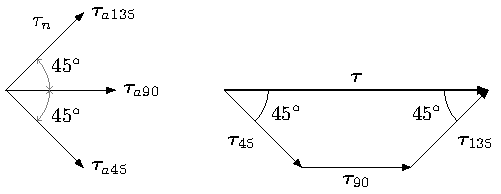
\includegraphics{figRotatingMachPrinciplesDistributedWindingFactor}
\begin{subfigure}{0.45\textwidth}
\centering
\begin{tikzpicture}
\draw[-latex](0,0)--(0:\sRo)node[right]{${\bm{\tau}}_{a90}$};
\draw[-latex](0,0)--(45:\sRo)node[right]{${\bm{\tau}}_{a135}$}node[pos=0.7,above left]{$\tau_n$};
\draw[-latex](0,0)--(-45:\sRo)node[right]{${\bm{\tau}}_{a45}$};
\draw[gray,<->] (0:0.4*\sRo) arc (0:45:0.4*\sRo);
\draw node at (22.5:0.6*\sRo){$45\degree$};
\draw[gray,<->] (0:0.4*\sRo) arc (0:-45:0.4*\sRo);
\draw node at (-22.5:0.6*\sRo){$45\degree$};
\end{tikzpicture}
\end{subfigure}%
\begin{subfigure}{0.45\textwidth}
\centering
\begin{tikzpicture}
\draw[-latex](0,0)--(-45:\sRo)node[below left,pos=0.5]{${\bm{\tau}}_{45}$};
\draw[-latex](-45:\sRo)--++(0:\sRo)node[below,pos=0.5]{${\bm{\tau}}_{90}$};
\draw[-latex] (-45:\sRo)++(0:\sRo)--++(45:\sRo)node[below right,pos=0.5]{${\bm{\tau}}_{135}$} coordinate(netFlux);
\draw[thick,-latex](0,0)--(netFlux)node[above,pos=0.5]{${\bm{\tau}}$};
\draw(0:0.4*\sRo) arc (0:-45:0.4*\sRo);
\draw node at (-20:0.6*\sRo){$45\degree$};
\draw(netFlux)--++(180:0.4*\sRo) arc (180:225:0.4*\sRo);
\draw (netFlux)++(200:0.6*\sRo)node{$45\degree$};
\end{tikzpicture}
\end{subfigure}%
\caption{پھیلے لچھے کا جزو پھیلاو۔}
\label{شکل_گھومتے_مشین_جزو_پھیلاو}
\end{figure}

حل: \quad
شکل  \حوالہ{شکل_گھومتے_مشین_جزو_پھیلاو} سے رجوع کریں۔ شکل \حوالہ{شکل_گھومتے_مشین_پھیلا_لچھا} کے تین چھوٹے لچھے ایک جیسا  مقناطیسی دباو \عددیء{\tau_n=\tfrac{4}{\pi}\tfrac{ni}{2}} پیدا کرتے ہیں البتہ ان کے رخ مختلف ہیں۔یہاں ایک لچھا  \عددیء{\tfrac{N}{3}} چکر کا ہے لہٰذا \عددیء{n=\tfrac{N}{3}} ہو گا۔ ہم تینوں مقناطیسی دباو کے دوری سمتیات کا مجموعہ لے کر  مقناطیسی دباو \عددیء{\tau} معلوم کرتے ہیں۔
\begin{align*}
\tau_a&=\tau_n \cos 45\degree+\tau_n+\tau_n \cos 45\degree\\
&=2.4142 \tau_n
\end{align*}
یوں درج ذیل ہو گا
\begin{align*}
\tau_a=2.4142 \frac{4}{\pi}\frac{ni}{2}=\frac{2.4142}{3} \frac{4}{\pi}\frac{N i}{2}=0.8047 \frac{4}{\pi}\frac{N i}{2}
\end{align*}
لہٰذا \عددیء{k_w=0.8047} کے برابر ہے۔
\انتہا{مثال}
%
\ابتدا{مثال}
تین دوری، \عددیء{50} ہرٹز، ستارہ جڑے جنریٹر کو  \عددیء{3000} چکر فی منٹ کی رفتار سے چلایا جاتا ہے۔تیس چکر کے میدانی لچھے  کا جزو پھیلاو \عددیء{k_{w,m}=0.9} جبکہ پندرہ چکر قوی لچھے کا جزو پھیلاو \عددیء{k_{w,q}=0.833} ہے۔مشین کا رداس \عددیء{0.7495} میٹر اور لمبائی \عددیء{l=2.828} میٹر ہے۔خلائی درز کی لمبائی \عددیء{l_k=0.04} میٹر ہے۔میدانی لچھے میں \عددیء{1000}  ایمپیئر برقی رو کی صورت میں درج ذیل تلاش کریں۔
\begin{itemize}
\item
میدانی مقناطیسی دباو کی زیادہ سے زیادہ قیمت۔
\item
خلائی درز میں کثافت مقناطیسی بہاو۔
\item
ایک قطب پر مقناطیسی بہاو۔
\item
متحرک تار پر برقی دباو۔
\end{itemize}

حل:
\begin{itemize}
\item
\(
\tau_0=k_{w,m} \frac{4}{\pi}\frac{N_m i_m}{2}=0.9 \times \frac{4}{\pi} \times \frac{30 \times 1000}{2}=\SI{17186}{\ampere \cdot turns \per \meter}
\)
\item
\(
B_0=\mu_0 H_0=\mu_0 \frac{\tau_0}{l_k}=4 \pi 10^{-7} \times \frac{17186}{0.04}=\SI{0.54}{\tesla}
\)
\item
\(
\phi_0=2 B_0 l r =2 \times 0.54 \times 2.828 \times 0.7495=\SI{2.28915}{\weber}
\)
\item
\begin{align*}
E_{rms}&=4.44 f k_{w,q} N_q \phi_0\\
&=4.44 \times 50 \times 0.833 \times 15 \times 2.28915\\
&=\SI{6349.85}{\volt} 
\end{align*}
\end{itemize}
یوں ستارہ جڑی جنریٹر کی تار کا برقی دباو درج ذیل ہو گا۔
\begin{align*}
\sqrt{3} \times 6349.85 \approx \SI{11000}{\volt}
\end{align*}
\انتہا{مثال}
%
ہم  سائن نما مقناطیسی دباو حاصل کرنا چاہتے ہیں۔ چھوٹے لچھوں کے چکر اور شگافوں کے مقامات یوں چنے جاتے ہیں کہ یہ مقصد پورا ہو۔ شکل \حوالہ{شکل_گھومتے_مشین_پھیلے_لچھے_نقطہ_صلیب_پر_جمپ}  میں  صفر زاویہ کے دونوں اطراف مقناطیسی دباو کی ترسیم ایک جیسے گھٹتی یا بڑھتی ہے۔ مثلاً جمع اور منفی  پینتالیس زاویہ پر مقناطیسی دباو  \عددیء{\tfrac{Ni}{3}}  گھٹتا ہے۔ اسی طرح جمع اور منفی نوے زاویہ پر دباو مزید \عددیء{\tfrac{Ni}{3}}  گھٹتا ہے، وغیرہ وغیرہ۔ یہ ایک بنیادی اصول ہے جس کا خیال رکھنا ضروری ہے۔

چھوٹے لچھوں کے چکر اور شگافوں کے مقامات کا فیصلہ فوریئر تسلسل کی مدد سے کیا جاتا ہے۔فوریئر تسلسل میں موسیقائی جزو  کم سے کم اور بنیادی جزو  زیادہ سے زیادہ رکھا جاتا ہے۔

ساکن لچھوں کی طرح متحرک لچھوں کو بھی ایک سے زیادہ چھوٹے لچھوں میں تقسیم کیا جاتا ہے تا کہ سائن نما مقناطیسی دباو حاصل ہو۔

\حصہ{مقناطیسی دباو کی گھومتی امواج}
گھومتے مشین کے لچھوں کو برقی دباو فراہم کیا جاتا ہے جس سے اس کا گھومنے والا حصہ حرکت میں آتا ہے۔ یہاں ہم اس بات کا مطالعہ کرتے ہیں کہ گھومنے کی حرکت کیسے پیدا ہوتی ہے۔

\جزوحصہ{ایک دور کی لپٹی مشین}
مساوات \حوالہ{مساوات_گھومتے_مشین_دباو_سائن_نما}  میں ایک لچھے کا مقناطیسی دباو
\begin{align}
\tau_a=k_w \frac{4}{\pi}\frac{Ni}{2} \cos \theta
\end{align}
دیا گیا ہے جو  سائن نما برقی رو
\begin{align}
i_a&=I_0 \cos \omega t
\end{align}
کی صورت میں
\begin{align}\label{مساوات_گھومتے_مشین_دباو_زاویہ_اور_وقت_پر_منحصر}
\tau_a=k_w \frac{4}{\pi} \frac{N I_0}{2} \cos \theta \cos \omega t=\tau_0 \cos \theta \cos \omega t
\end{align}
مقناطیسی دباو دے گا جہاں \عددی{\tau_0} درج ذیل ہے اور لچھا کے برقی رو کو \عددی{i_a} کہا گیا ہے۔
\begin{align}
\tau_0=k_w \frac{4}{\pi} \frac{N I_0}{2}
\end{align}
مساوات \حوالہ{مساوات_گھومتے_مشین_دباو_زاویہ_اور_وقت_پر_منحصر}  کہتی ہے کہ  مقناطیسی دباو زاویہ \عددیء{\theta} اور لمحہ \عددیء{t} کے ساتھ تبدیل ہوتا ہے۔ مساوات \حوالہ{مساوات_گھومتے_مشین_دباو_زاویہ_اور_وقت_پر_منحصر} کو کلیہ 
\begin{align}\label{مساوات_گھومتے_مشین_کو_سائن_ٹکڑے}
\cos \alpha \cos \beta =\frac{\cos (\alpha +\beta) +\cos (\alpha -\beta)}{2}
\end{align}
کی مدد سے دو ٹکڑوں 
\begin{align}\label{مساوات_گھومتے_مشین_دو_مخالف_گھومتے_اجزاء}
\tau_a=\tau_0 \left [\frac{\cos (\theta +\omega t) +\cos (\theta -\omega t)}{2}\right]=\tau_a^{-}+\tau_a^{+}
\end{align}
میں تقسیم کیا جا سکتا ہے جہاں \عددی{\tau_a^{-}} اور \عددی{\tau_a^{+}} درج ذیل ہوں گے۔
\begin{align}
\tau_a^{-}&=\frac{\tau_0}{2} \cos (\theta +\omega t)\\
\tau_a^{+}&=\frac{\tau_0}{2} \cos (\theta -\omega t)
\end{align}
مساوات \حوالہ{مساوات_گھومتے_مشین_دو_مخالف_گھومتے_اجزاء}  کہتی ہے کہ  مقناطیسی دباو دو آپس میں مخالف رخ گھومتے  مقناطیسی دباو کی موجوں کا مجموعہ ہے۔ اس کا پہلا جزو \عددیء{\tau_a^-} زاویہ \عددیء{\theta} گھٹنے کے رخ،  یعنی گھڑی کے رخ ، گھومتا ہے جبکہ اس کا دوسرا جزو \عددیء{\tau_a^+} گھڑی کے مخالف رخ، زاویہ بڑھنے کے رخ،  گھومتا ہے۔

ایک دور کی لپٹی مشینوں میں گھومتے مقناطیسی دباو کی امواج میں سے کسی ایک کو بالکل ختم یا کم سے کم کرنے کی کوشش کی جاتی ہے۔ اس طرح ایک ہی رخ  مقناطیسی دباو گھومتا ملے گا جو بالکل  ایک گھومتے ہوئے  مقناطیس کی مانند ہو گا۔ تین دوری  مشینوں میں ایسا کرنا نہایت آسان ہوتا ہے لہٰذا انہیں پہلے سمجھ لینا زیادہ بہتر ہو گا۔

\جزوحصہ{تین دور کی لپٹی مشین کا تحلیلی تجزیہ}
شکل \حوالہ{شکل_گھومتے_مشین_تین_دور_کے_لئے_لپٹی}  میں تین دور کی لپٹی مشین دکھائی گئی ہے۔مساوات \حوالہ{مساوات_گھومتے_مشین_الف_موج} ، \حوالہ{مساوات_گھومتے_مشین_ب_موج}  اور \حوالہ{مساوات_گھومتے_مشین_پ_موج}  میں ایسے تین لچھوں کے فوریئر تسلسل کے بنیادی اجزاء دیے گئے ہیں جن میں جزو پھیلاو \عددی{k_x} شامل کر کے دوبارہ پیش کرتے ہیں۔
\begin{gather}
\begin{aligned}\label{مساوات_گھومتے_مشین_تین_دباو_الف}
\tau_a&=k_w \frac{4}{\pi}\frac{N_a i_a}{2}\cos \theta\\
\tau_b&=k_w \frac{4}{\pi}\frac{N_b i_b}{2}\cos (\theta-120\degree)\\
\tau_c&=k_w \frac{4}{\pi}\frac{N_c i_c}{2}\cos (\theta+120\degree)
\end{aligned}
\end{gather}
%
\begin{figure}
\centering
%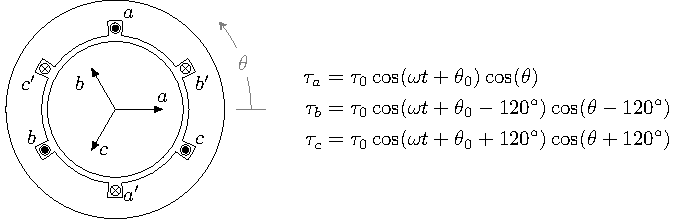
\includegraphics{figRotatingMachPrinciplesThreePhaseSynchronousMachine}
\begin{tikzpicture}
\pgfmathsetmacro{\shiftX}{5cm}
\stator{6}{30}
\slotDot{90,210,330}
\slotCross{30,150,270}
%\slotName{comma separated angles/name/NameAtleftORrightOfSlot}
\slotName{90/a/above right,210/b/above left,330/c/above right}
\slotName{30/b'/below right,150/c'/below left,270/a'/right}
%
\draw (0,0) circle (\rR);
\draw[-latex] (0,0)--++(0:0.7*\rR)node [above]{$a$};
\draw[-latex] (0,0)--++(120:0.7*\rR)node [below left]{$b$};
\draw[-latex] (0,0)--++(-120:0.7*\rR)node [right]{$c$};
%
\draw[](0:\sRo+0.2)--++(0:0.5 )coordinate[pos=0.5] (angleZero);
\draw[-stealth](angleZero) arc (0:40:\sRo+0.2+0.25);
\draw node[fill=white] at (20:\sRo+0.2+0.25){$\theta$};
%
\draw node[right] at (3,0){$\begin{aligned}
\tau_a&=\tau_0 \cos (\omega t+\theta_0) \cos (\theta)\\
\tau_b&=\tau_0 \cos (\omega t+\theta_0-120\degree) \cos (\theta-120\degree)\\
\tau_c&=\tau_0 \cos (\omega t+\theta_0+120\degree) \cos (\theta+120\degree)
\end{aligned}
$};
\end{tikzpicture}
\caption{تین دور کی لپٹی مشین۔}
\label{شکل_گھومتے_مشین_تین_دور_کے_لئے_لپٹی}
\end{figure}
ان لچھوں میں بالترتیب تین دوری برقی رو 
\begin{gather}
\begin{aligned}\label{مساوات_گھومتے_مشین_تین_برقی_رو}
i_a&=I_0 \cos (\omega t+\alpha)\\
i_b&=I_0 \cos (\omega t +\alpha -120\degree)\\
i_c&=I_0 \cos (\omega t +\alpha +120\degree)
\end{aligned}
\end{gather}
لینے سے  مساوات \حوالہ{مساوات_گھومتے_مشین_تین_دباو_الف} درج ذیل صورت اختیار کرتی ہیں۔
\begin{gather}
\begin{aligned}
\tau_a&=k_w \frac{4}{\pi}\frac{N_a I_0}{2} \cos \theta \cos (\omega t +\alpha)\\
\tau_b&=k_w \frac{4}{\pi}\frac{N_b I_0}{2} \cos (\theta -120\degree)\cos (\omega t +\alpha -120\degree)\\
\tau_c&=k_w \frac{4}{\pi}\frac{N_c I_0}{2} \cos (\theta +120\degree)\cos (\omega t +\alpha +120\degree)
\end{aligned}
\end{gather}
تینوں لچھوں کے چکر ایک دوسرے کے برابر
\begin{align*}
N_a=N_b=N_c=N
\end{align*}
لیتے ہوئے مساوات \حوالہ{مساوات_گھومتے_مشین_کو_سائن_ٹکڑے} کی استعمال سے
\begin{gather}
\begin{aligned}\label{مساوات_تبادلہ_تین_گھومتے_دباو}
\tau_a&=\frac{\tau_0}{2} \left[\cos (\theta +\omega t +\alpha) +\cos (\theta -\omega t -\alpha) \right]\\
\tau_b&=\frac{\tau_0}{2} \left[\cos (\theta +\omega t +\alpha-240\degree) +\cos (\theta -\omega t -\alpha) \right]\\
\tau_c&=\frac{\tau_0}{2} \left[\cos (\theta +\omega t +\alpha+240\degree) +\cos (\theta -\omega t -\alpha) \right]
\end{aligned}
\end{gather}
لکھے جا سکتے ہیں جہاں \عددی{\tau_0} درج ذیل ہے۔
\begin{align}
\tau_0=k_w \frac{4}{\pi}\frac{N I_0}{2}
\end{align}
کل مقناطیسی دباو \عددیء{\tau} ان سب کا مجموعہ ہو گا۔ انہیں جمع کرنے سے پہلے ہم  درج ذیل ثابت کرتے ہیں۔
\begin{align*}
\cos \gamma +\cos (\gamma -240\degree)+\cos (\gamma+240\degree)=0
\end{align*}
ہم  کلیات 
\begin{align*}
\cos  (\alpha +\beta)&=\cos \alpha \cos \beta-\sin \alpha \sin \beta\\
\cos  (\alpha -\beta)&=\cos \alpha \cos \beta+\sin \alpha \sin \beta
\end{align*}
 میں  \عددیء{\alpha = \gamma} اور \عددیء{\beta=240\degree} لے کر
\begin{align*}
\cos (\gamma+240\degree)&=\cos \gamma \cos 240\degree-\sin \gamma \sin 240\degree\\
\cos (\gamma-240\degree)&=\cos \gamma \cos 240\degree+\sin \gamma \sin 240\degree
\end{align*}
حاصل کرتے ہیں جن میں  \عددیء{\cos 240\degree=-\tfrac{1}{2}} اور \عددیء{\sin 240\degree=-\tfrac{\sqrt{3}}{2}} پر کر کے درج ذیل حاصل ہو گا۔
\begin{align*}
\cos (\gamma+240\degree)&=-\frac{1}{2}\cos \gamma +\frac{\sqrt{3}}{2}\sin \gamma\\
\cos (\gamma-240\degree)&=-\frac{1}{2}\cos \gamma -\frac{\sqrt{3}}{2}\sin \gamma
\end{align*}
ان مساوات کو   \عددیء{\cos \gamma} کے ساتھ جمع کرنے سے  صفر حاصل ہو گا۔
\begin{align*}
\cos \gamma +\cos (\gamma+240\degree)+\cos (\gamma-240\degree)=0
\end{align*}
\عددیء{\gamma=\theta+\omega t +\alpha} کے لئے اس مساوات کو درج ذیل لکھا جا سکتا ہے۔
\begin{align}\label{مساوات_تبادلہ_تین_سمتیات_جمع_صفر}
\cos (\theta +\omega t +\alpha) +\cos (\theta +\omega t +\alpha+240\degree)+\cos (\theta+\omega t +\alpha-240\degree)=0
\end{align}
اب مساوات \حوالہ{مساوات_تبادلہ_تین_گھومتے_دباو}  میں دئے  \عددیء{\tau_a} ، \عددیء{\tau_b} اور \عددیء{\tau_c}  کو جمع کر کے مساوات \حوالہ{مساوات_تبادلہ_تین_سمتیات_جمع_صفر}  کا استعمال کرتے ہوئے درج ذیل حاصل ہو گا۔
\begin{align}\label{مساوات_تبادلہ_گھومتا_موج}
\tau^+=\tau_a+\tau_b+\tau_c=\frac{3 \tau_0}{2} \cos (\theta -\omega t -\alpha)
\end{align}
مساوات \حوالہ{مساوات_تبادلہ_گھومتا_موج} کہتی ہے کہ کل مقناطیسی دباو کا حیطہ کسی ایک لچھے کے مقناطیسی دباو کے حیطہ کا \عددیء{\tfrac{3}{2}} گنا ہو گا۔مزید مقناطیسی دباو کی موج گھڑی کے مخالف رخ گھومے گی۔ یوں  تین لچھوں کو \عددیء{120\degree}  زاویہ پر رکھنے اور انہیں تین دوری برقی رو، جو آپس میں \عددیء{120\degree} پر ہوں،  سے  ہیجان کرنے سے  مقناطیسی دباو کی واحد ایک موج وجود میں آتی ہے۔ یہاں اس بات کا ذکر کرنا ضروری ہے کہ  کسی دو برقی رو کو آپس میں تبدیل کرنے سے مقناطیسی موج کا رخ تبدیل ہوتا ہے۔  

مساوات \حوالہ{مساوات_تبادلہ_گھومتا_موج} ایک گھومتے موج کو ظاہر کرتی ہے جس میں ہم برقی رو کا تعدد  \عددیء{\SI{50}{\hertz}} اور اپنی آسانی کے لئے \عددیء{\alpha}  کو صفر لیتے ہیں۔  یوں اس موج کی چوٹی کا تعین تفاعل \عددیء{\cos (\theta -\omega t)} کرے گا۔  تفاعل \عددیء{\cos (\theta -\omega t)} کی چوٹی پر نظر رکھیں۔ تفاعل \عددیء{\cos (\theta -\omega t)} کی چوٹی اکائی ہے جو \عددی{\theta-\omega t=0} پر پائی جاتی ہے۔

ابتدائی لمحہ \عددیء{t=0} پر \عددیء{\cos (\theta -\omega t)} کی چوٹی \عددیء{(\theta-\omega t)=0} پر ہو گی جس کو \عددی{t=0} کے لئے  حل کرتے ہیں۔
\begin{align*}
\theta-\omega t &=0\\
\theta -\omega \times 0&=0\\
\theta& =0
\end{align*}
%
\begin{figure}
\centering
\begin{tikzpicture}]
\pgfmathsetmacro{\tc}{160}
\begin{axis}[clip=false,small,axis lines=middle, xlabel={$\theta_e$},xtick={18,\tc},xticklabels={$\tfrac{\pi}{10}$,$\omega t'$},ytick={\empty},enlargelimits=true,xlabel style={at={(current axis.right of origin)},anchor=west},axis line style={-}]
\addplot[dashed,domain=-90:270,smooth](x,{cos(x-0)});
\addplot[domain=-90+18:270+18,smooth](x,{cos(x-18)});
\addplot[thick,domain=-90+\tc:270+\tc,smooth](x,{cos(x-\tc)});
\draw(axis cs:0,1)node[pin=145:{$t=0$}]{};
\draw(axis cs:18,1)node[pin=60:{$t=0.001$}]{};
\draw(axis cs:\tc,1)node[pin={[right]35:{$t=t'$}}]{};
\addplot[dashed] coordinates {(18,0)(18,1)};
\addplot[dashed] coordinates {(\tc,0)(\tc,1)};
\end{axis}
\end{tikzpicture}
\caption{حرکت کرتی موج۔}
\label{شکل_گھومتے_مشین_حرکت_کرتی_موج}
\end{figure}
یوں موج کی چوٹی صفر برقی زاویہ پر ہو گی جسے شکل \حوالہ{شکل_گھومتے_مشین_حرکت_کرتی_موج} میں  نقطہ دار لکیر سے ظاہر کیا گیا ہے۔ہم  کچھ وقفہ، مثلاً \عددیء{t=0.001} سیکنڈ، بعد اس چوٹی پر   دوبارہ نظر ڈالتے ہیں۔
\begin{align*}
\theta-\omega t &=0\\
\theta -0.001 \omega &=0\\
\theta &=0.001 \omega \\
&=0.001 \times 2 \times \pi \times 50\\
&=\SI{0.3142}{\radian} 
\end{align*}
اب یہ چوٹی \عددیء{0.3142} یا \عددیء{\tfrac{\pi}{10}} برقی ریڈیئن یعنی \عددیء{18\degree}  برقی زاویہ پر ہے جسے شکل \حوالہ{شکل_گھومتے_مشین_حرکت_کرتی_موج} میں باریک  ٹھوس لکیر سے ظاہر کیا گیا ہے۔ آپ دیکھ سکتے ہیں کہ مقناطیسی دباو کی موج گھڑی کے مخالف رخ، یعنی زاویہ بڑھنے کے رخ،  گھوم گئی ہے۔ اسی طرح لمحہ \عددیء{t=0.002}  پر چوٹی \عددیء{36\degree} برقی زاویہ پر نظر آئے گی۔عمومی  لمحہ \عددیء{t'} پر  چوٹی کا مقام \عددی{\theta-\omega t' =0}  سے درج ذیل  حاصل ہو گا جسے موٹی ٹھوس لکیر سے ظاہر کیا گیا ہے۔
\begin{align}\label{مساوات_گھومتا_مشین_چوٹی_کا_مقام}
\theta &=\omega t'
\end{align}


مساوات \حوالہ{مساوات_گھومتا_مشین_چوٹی_کا_مقام}  کہتی ہے  کہ چوٹی کا مقام تعین کرنے والا زاویہ وقت کے ساتھ  بتدریج بڑھتا  ہے۔اس مساوات سے  ایک مکمل \عددیء{2\pi} برقی زاویہ  چکر کا دورانیہ \عددیء{T} حاصل کرتے ہیں۔
\begin{gather}
\begin{aligned}\label{مساوات_گھومتے_مشین_دوری_وقفہ}
T&=\frac{\theta}{\omega}=\frac{2\pi}{2\pi f}=\frac{1}{f}
\end{aligned}
\end{gather}
یاد رہے \عددی{f} برقی رو کی تعدد ہے۔یوں \عددیء{50} ہرٹز برقی رو کی صورت میں مقناطیسی دباو کی موج ہر \عددیء{\tfrac{1}{50}=0.02} سیکنڈ میں ایک مکمل برقی چکر   لہٰذا  ایک سیکنڈ میں \عددیء{50} برقی چکر مکمل کرے گی۔

دو قطبی مشینوں میں مساوات \حوالہ{مساوات_گھومتے_مشین_برقی_میکانی_زاویہ_تعلق}
\begin{align}
\theta_e=\frac{P}{2} \theta_m
\end{align}
 کے تحت  برقی زاویہ \عددیء{\theta_e}  اور میکانی زاویہ \عددیء{\theta_m} ایک دوسرے کے برابر ہوں گے۔ یوں دو قطبی مشینوں کی بات کرتے ہوئے  مساوات \حوالہ{مساوات_گھومتے_مشین_دوری_وقفہ}  کے تحت ایک سیکنڈ میں مقناطیسی دباو کی موج \عددیء{f} برقی یا میکانی چکر مکمل کرے  گی جہاں \عددیء{f} برقی رو کی تعدد ہے۔  \عددیء{P} قطبی مشینوں  کے مقناطیسی دباو کی موج ایک سیکنڈ میں \عددیء{f} مقناطیسی چکر یعنی \عددیء{\tfrac{2}{P}f} میکانی شکر مکمل کرے گی۔

برقی رو کی تعدد کو \عددیء{f_e}، مقناطیسی دباو کی موج کی چوٹی کے برقی زاویہ کو \عددیء{\theta_e}،  میکانی زاویہ کو \عددیء{\theta_m}  اور  مقناطیسی دباو کی موج کی زاویائی رفتار کو \عددیء{\omega_e} یا \عددیء{\omega_m} سے ظاہر کرتے ہوئے درج ذیل ہوں گے۔
\begin{gather}
\begin{aligned}\label{مساوات_گھومتے_مشین_برقی_میکانی_رفتار_تعلق}
\omega_m&=\frac{2}{P} \omega_e \quad \si{\radian / \second}\\
f_m&=\frac{2}{P} f_e \quad \si{\hertz}\\
n&=\frac{120 f_e}{P} \quad  \text{\RL{چکر فی سیکنڈ}}
\end{aligned}
\end{gather}
مقناطیسی  موج کی برقی معاصر زاویائی رفتار \عددیء{\omega_e}   برقی زاویہ فی سیکنڈ اور میکانی معاصر زاویائی رفتار  \عددیء{\omega_m}  میکانی زاویہ فی سیکنڈ  ہو گی۔اسی طرح موج کی برقی  معاصر رفتار  \عددیء{f_e} برقی ہرٹز اور میکانی \اصطلاح{معاصر رفتار}\فرہنگ{معاصر رفتار}\حاشیہب{synchronous speed}\فرہنگ{synchronous speed} \عددیء{f_m} میکانی ہرٹز ہو گی۔برقی معاصر رفتار \عددیء{f_e}  ہرٹز ہونے سے مراد  ہے کہ ایک سیکنڈ میں  موج \عددیء{f_e} برقی چکر کا فاصلہ طے کرتی ہے جو دو قطب کا یعنی \عددیء{2\pi}  ریڈیئن کا میکانی  زاویہ ہے۔اسی طرح میکانی معاصر رفتار \عددیء{f_m} ہرٹز ہونے کا مطلب ہے کہ  موج ایک سیکنڈ میں \عددیء{f_m} میکانی چکر کا فاصلہ طے کرے گی۔ایک میکانی چکر روز مرہ  زندگی میں ایک چکر کو ہی کہتے ہیں۔ اس مساوات میں \عددیء{n}، میکانی \اصطلاح{چکر فی منٹ}\فرہنگ{rpm}\حاشیہب{rpm, rounds per minute}  کو ظاہر کرتی ہے۔ مساوات \حوالہ{مساوات_گھومتے_مشین_برقی_میکانی_رفتار_تعلق} \اصطلاح{معاصر رفتار}\فرہنگ{معاصر رفتار}\فرہنگ{synchronous speed} کی مساوات ہے۔

یہاں اس بات کا ذکر کرنا ضروری ہے کہ \عددیء{q} دور کی لپٹی مشین جس کے لچھے \عددیء{\tfrac{2\pi}{q}} برقی زاویہ پر رکھے گئے ہوں اور جن میں برقی رو  \عددیء{q}  دوری  ہو میں، تین دوری مشین  کی طرح، ایک ہی رخ گھومتے  مقناطیسی دباو کی  موج  پیدا ہو گی۔مزید، اس موج کا حیطہ کسی ایک لچھے کے مقناطیسی دباو کے حیطہ  کا \عددیء{\tfrac{q}{2}}  گنا ہو گا اور اس کی زاویائی  رفتار \عددیء{\omega_e=2\pi f} برقی ریڈیئن فی سیکنڈ ہو گی۔

\جزوحصہ{تین دور کی لپٹی مشین کا ترسیمی تجزیہ}
شکل \حوالہ{شکل_گھومتے_مشین_تین_دوری}  میں تین دور کی لپٹی مشین دکھائی گئی ہے جس میں مثبت برقی رو کے رخ  دکھائے گئے ہیں۔یوں  \عددیء{a} شگاف میں برقی رو کا رخ صفحہ سے عمودی  باہر کو  ہے  جسے نقطہ سے ظاہر کیا گیا ہے۔ اسی طرح \عددیء{a'} شگاف میں برقی رو کا رخ صفحہ میں عمودی  اندر  کو ہے اور  جسے صلیب کے نشان سے ظاہر کیا گیا ہے۔یوں شگاف \عددیء{a} اور\عددیء{a'}  میں مثبت برقی رو کا مقناطیسی دباو \عددیء{\سمتیہ{\tau}_a} صفر زاویہ پر ہو گا جو عین لچھا \عددی{a} کا رخ  ہے۔ لچھے میں برقی رو سے پیدا مقناطیسی دباو  کا رخ دائیں ہاتھ کے قانون سے معلوم کیا جا سکتا ہے۔

 اب اگر لچھا \عددی{a} میں برقی رو منفی ہو تب برقی رو مثبت رخ کے مخالف ہو گا، یعنی اب برقی رو کا رخ  شگاف  \عددیء{a} میں صفحہ کے عمودی  اندر  اور شگاف \عددیء{a'}  میں  صفحہ کے عمودی  باہر ہو گا۔ یوں منفی برقی رو سے پیدا مقناطیسی دباو بھی لچھا \عددی{a} کے رخ کا  مخالف ہو گا۔آپ نے دیکھا کہ برقی رو منفی ہونے سے مقناطیسی دباو کا رخ الٹ ہو جاتا ہے۔
\begin{figure}
\centering
%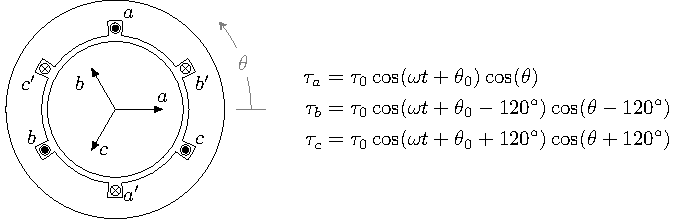
\includegraphics{figRotatingMachPrinciplesThreePhaseSynchronousMachine}
\begin{tikzpicture}
%grid
%\draw[gray] (-\sRo,-\sRo) grid (\sRo,\sRo);
\pgfmathsetmacro{\shiftX}{5cm}
\stator{6}{30}
\slotDot{90,210,330}
\slotCross{30,150,270}
%\slotName{comma separated angles/name/NameAtleftORrightOfSlot}
\slotName{90/a/above right,210/b/above left,330/c/above right}
\slotName{30/b'/below right,150/c'/below left,270/a'/right}
%
\draw (0,0) circle (\rR);
\draw[-latex] (0,0)--++(0:0.7*\rR)node [above]{$\tau_a$};
\draw[-latex] (0,0)--++(120:0.7*\rR)node [below left]{$\tau_b$};
\draw[-latex] (0,0)--++(-120:0.7*\rR)node [right]{$\tau_c$};
%
\draw[](0:\sRo+0.2)--++(0:0.5 )coordinate[pos=0.5] (angleZero);
\draw[-stealth](angleZero) arc (0:40:\sRo+0.2+0.25);
\draw node[fill=white] at (20:\sRo+0.2+0.25){$\theta$};
\end{tikzpicture}
\caption{تین دور کی لپٹی مشین میں مثبت برقی رو اور ان سے حاصل مقناطیسی دباو کے رخ۔}
\label{شکل_گھومتے_مشین_تین_دوری}
\end{figure}
شکل \حوالہ{شکل_گھومتے_مشین_تین_دوری} میں لچھوں کے برقی رو اور مقناطیسی دباو درج ذیل ہیں جبکہ ان کے مثبت رخ شکل میں دیے گئے ہیں۔
\begin{gather}
\begin{aligned}\label{مساوات_گھومتے_مشین_تین_دور_برقی_رو}
i_a&=I_0 \cos \omega t\\
i_b&=I_0 \cos (\omega t-120\degree)\\
i_c&=I_0 \cos (\omega t+120\degree)
\end{aligned}
\end{gather}
%
\begin{gather}
\begin{aligned}\label{مساوات_گھومتے_مشین_تین_دور_دباو}
\tau_a&=k_w \frac{4}{\pi}\frac{N i_a}{2}=k_w \frac{4}{\pi}\frac{N I_0}{2} \cos \omega t=\tau_0 \cos \omega t\\
\tau_b&=k_w \frac{4}{\pi}\frac{N i_b}{2}=k_w \frac{4}{\pi}\frac{N I_0}{2} \cos (\omega t-120\degree)=\tau_0 \cos (\omega t-120\degree)\\
\tau_c&=k_w \frac{4}{\pi}\frac{N i_c}{2}=k_w \frac{4}{\pi}\frac{N I_0}{2} \cos (\omega t+120\degree)=\tau_0 \cos (\omega t+120\degree)
\end{aligned}
\end{gather}
 ہم مختلف لمحات پر ان کی قیمتوں  تلاش کرتے ہیں اور ان کا مجموعی مقناطیسی دباو حاصل کرتے ہیں۔

لمحہ \عددیء{t=0} پر ان درج بالا مساوات سے درج ذیل حاصل ہو گا۔
\begin{gather}
\begin{aligned}
i_a&=I_0 \cos 0=I_0\\
i_b&=I_0 \cos (0-120\degree)=-0.5 I_0\\
i_c&=I_0 \cos (0+120\degree)=-0.5 I_0
\end{aligned}
\end{gather}
%
\begin{gather}
\begin{aligned}
\tau_a&=\tau_0 \cos 0=\tau_0\\
\tau_b&=\tau_0 \cos (0-120\degree)=-0.5 \tau_0\\
\tau_c&=\tau_0 \cos (0+120\degree)=-0.5 \tau_0
\end{aligned}
\end{gather}
یہاں رکھ کر ذرا غور کریں۔لمحہ \عددی{t=0}  پر  \عددیء{i_a} مثبت  جبکہ \عددیء{i_b} اور \عددیء{i_c} منفی ہیں۔ یوں \عددیء{i_a}  کا رخ وہی  ہو گا جسے  شکل  \حوالہ{شکل_گھومتے_مشین_تین_دوری} کی  \عددیء{a} اور \عددیء{a'} شگافوں میں نقطے اور صلیب سے  دکھایا گیا ہیں جبکہ  \عددیء{i_b} اور \عددیء{i_c} کے رخ شکل میں دیے گئے رخ کے مخالف ہوں گے۔ لمحہ \عددی{t=0} پر  تینوں برقی رو کے درست رخ اور  تینوں مقناطیسی دباو  شکل \حوالہ{شکل_گھومتے_مشین_لمحہ_صفر_پر_کل_دباو}  میں دکھائے گئے ہیں۔
\begin{figure}
\centering
%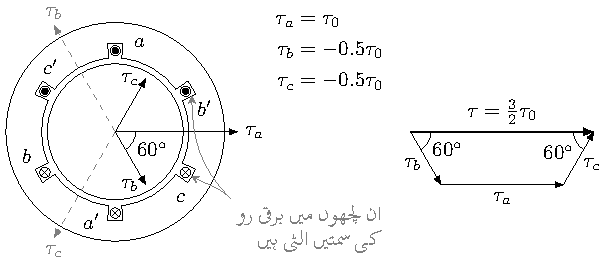
\includegraphics{figRotatingMachPrinciplesThreePhaseFluxAtTimeZero}
\begin{subfigure}{0.50\textwidth}
\centering
\begin{tikzpicture}
\stator{6}{30}
\slotDot{90,30,150}
\slotCross{-30,-90,-150}
\draw (0,0) circle (\rR);
%\slotName{45/a_1/,-45/a_1'/below,135/a_2'/,-135/a_2/below}
\draw (90-15:\sRi+1.25*\delR)node[]{$a$};
\draw (270-15:\sRi+1.25*\delR)node[]{$a'$};
\draw (210-15:\sRi+1.25*\delR)node[]{$b$};
\draw (30-15:\sRi+1.25*\delR)node[]{$b'$};
\draw (-30-15:\sRi+1.25*\delR)node[]{$c$};
\draw (150-15:\sRi+1.25*\delR)node[]{$c'$};
%
\draw[-latex](0,0)--(0:1.8*\rR)node[right]{$\tau_a$};
\draw[dashed,-latex](0,0)--(120:1.8*\rR)node[above]{$\tau_b$};
\draw[dashed,-latex](0,0)--(-120:1.8*\rR)node[below]{$\tau_c$};
\draw[-latex](0,0)--(-60:0.9*\rR)node[left]{$\tau_b$};
\draw[-latex](0,0)--(60:0.9*\rR)node[left]{$\tau_c$};
\draw (-60:0.3*\rR) arc (-60:0:0.3*\rR);
\draw node at (-25:0.6*\rR){$60\degree$};
\draw[stealth-] (-30:\sRi cm+\delR cm )++(0,0) to [out=-30,in=135]++(-30:0.6*\sRi)coordinate(reversedText);
\draw[stealth-] (30:\sRi cm+\delR cm )++(0,-0.15cm) to [out=-90,in=135](reversedText)node[below right,align=right]{\RL{ان لچھوں میں برقی رو} \\ \RL{ کے رخ ایک دوسرے}\\  \RL{کے مخالف ہیں}};
\end{tikzpicture}
\end{subfigure}%
\begin{subfigure}{0.40\textwidth}
\centering
\begin{tikzpicture}
\draw node[above] at (2*\rR,1){$\begin{aligned}
\tau_a&=\tau_0\\
\tau_b&=-0.5 \tau_0\\
\tau_c&=-0.5 \tau_0
\end{aligned}$};
\draw[-latex](0,0)--++(-60:0.9*\rR)node[pos=0.6,left]{$\tau_b$}coordinate(tipB);
\draw[-latex](tipB)--++(0:1.8*\rR)node[pos=0.5,below]{$\tau_a$}coordinate(tipA);
\draw[-latex](tipA)--++(60:0.9*\rR)node[pos=0.4,right]{$\tau_c$}coordinate(tipC);
\draw[-latex,thick](0,0)--(tipC)node[pos=0.5,above]{$\tau=\tfrac{3}{2} \tau_0$};
\draw (-60:0.3*\rR) arc (-60:0:0.3*\rR);
\draw node at (-25:0.6*\rR){$60\degree$};
\draw (tipC)++(180:0.3*\rR) arc (180:240:0.3*\rR);
\draw (tipC)++(210:0.6*\rR)node{$60\degree$};
\end{tikzpicture}
\end{subfigure}%
\caption{ لمحہ \عددیء{t_0=0} پر برقی رو اور مقناطیسی دباو۔}
\label{شکل_گھومتے_مشین_لمحہ_صفر_پر_کل_دباو}
\end{figure}

کل مقناطیسی دباو با آسانی بذریعہ ترسیم (شکل \حوالہ{شکل_گھومتے_مشین_لمحہ_صفر_پر_کل_دباو})،  مجموعہ سمتیات سے   یا  الجبرا کے ذریعہ حاصل کیا جا سکتا ہے۔
\begin{gather}
\begin{aligned}
\kvec{\tau}_a&=\tau_0 \ax\\
\kvec{\tau}_b&=0.5 \tau_0 \left[\cos (60\degree) \ax-\sin (60\degree)\ay \right]\\
\kvec{\tau}_c&=0.5 \tau_0 \left[\cos (60\degree) \ax+\sin (60\degree)\ay \right]
\end{aligned}
\end{gather}
ان کا مجموعہ درج ذیل ہو گا۔
\begin{align}
\kvec{\tau}=\kvec{\tau}_a+\kvec{\tau}_b+\kvec{\tau}_c=\frac{3}{2} \tau_0 \ax
\end{align}
لمحہ \عددی{t=0} پر کل مقناطیسی دباو ایک لچھے کے مقناطیسی دباو کا ڈیڑھ گنا  اور  صفر زاویہ پر ہے۔

 اب ہم گھڑی کو چلنے دیتے ہیں اور کچھ وقفہ بعد لمحہ \عددیء{t_1} پر دوبارہ مقناطیسی دباو تلاش کرتے ہیں۔ مساوات \حوالہ{مساوات_گھومتے_مشین_تین_دور_برقی_رو}  اور مساوات \حوالہ{مساوات_گھومتے_مشین_تین_دور_دباو}  میں متغیر \عددیء{t} کی بجائے \عددیء{\omega t} کا استعمال زیادہ آسان ہے لہٰذا ہم لمحہ \عددیء{t_1}  یوں منتخب کرتے ہیں کہ \عددیء{\omega t_1=30\degree}  ہو۔ ایسا کرنے سے  درج ذیل حاصل ہو گا جنہیں  شکل \حوالہ{شکل_گھموتے_مشین_وقت_تیس_پر_دباو}  میں دکھایا گیا ہے۔
\begin{figure}
\centering
%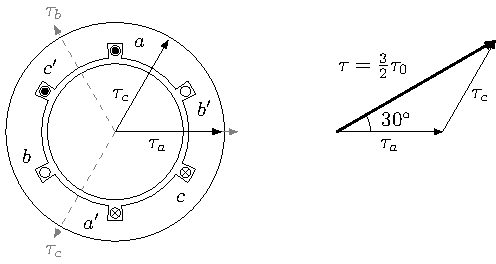
\includegraphics{figRotatingMachPrinciplesThreePhaseFluxAtTimeThirtyDegrees}
\begin{subfigure}{0.50\textwidth}
\centering
\begin{tikzpicture}
\stator{6}{30}
\slotDot{90,150}
\slotCross{-30,-90}
\slotEmptyCircle{30,210}
\draw (0,0) circle (\rR);
%
%\slotName{45/a_1/,-45/a_1'/below,135/a_2'/,-135/a_2/below}
\draw (90-15:\sRi+1.25*\delR)node[]{$a$};
\draw (270-15:\sRi+1.25*\delR)node[]{$a'$};
\draw (210-15:\sRi+1.25*\delR)node[]{$b$};
\draw (30-15:\sRi+1.25*\delR)node[]{$b'$};
\draw (-30-15:\sRi+1.25*\delR)node[]{$c$};
\draw (150-15:\sRi+1.25*\delR)node[]{$c'$};
%
\draw[dashed,-latex](0,0)--(120:1.8*\rR)node[above]{$\tau_b$};
\draw[dashed,-latex](0,0)--(-120:1.8*\rR)node[below]{$\tau_c$};
\draw[-latex](0,0)--(0:1.8*0.866*\rR)node[pos=0.4,below]{$\tau_a$};
%\draw[-latex](0,0)--(-60:0.9*\rR)node[left]{$\tau_b$};
\draw[-latex](0,0)--(60:1.8*0.866*\rR)node[pos=0.4,left]{$\tau_c$};
\end{tikzpicture}
\end{subfigure}%
\begin{subfigure}{0.40\textwidth}
\centering
\begin{tikzpicture}
\draw[-latex](0,0)--++(0:1.8*0.866*\rR)node[pos=0.5,below]{$\tau_a$}coordinate(tipA);
\draw[-latex](tipA)--++(60:1.8*0.866*\rR)node[pos=0.4,right]{$\tau_c$}coordinate(tipC);
\draw[-latex,thick](0,0)--(tipC)node[pos=0.5,above left]{ $\tau=\tfrac{3}{2}\tau_0$};
*
%\draw(tipA)++(60:0.2*\rR) arc (60:180:0.2*\rR);
%\draw (tipA)++(120:0.4*\rR)node{$120\degree$};
\draw(0:0.5*\rR) arc (0:30:0.5*\rR);
\draw node at (12:0.9*\rR){$30\degree$};
\end{tikzpicture}
\end{subfigure}%
\caption{ لمحہ \عددیء{\omega t_1=30\degree} پر برقی رو اور مقناطیسی دباو۔}
\label{شکل_گھموتے_مشین_وقت_تیس_پر_دباو}
\end{figure}
\begin{gather}
\begin{aligned}
i_a&=I_0 \cos 30\degree=\frac{\sqrt{3}}{2} I_0\\
i_b&=I_0 \cos (30\degree-120\degree)=0\\
i_c&=I_0 \cos (30\degree+120\degree)=-\frac{\sqrt{3}}{2} I_0
\end{aligned}
\end{gather}
%
\begin{gather}
\begin{aligned}
\tau_a&=\tau_0 \cos 30\degree=\frac{\sqrt{3}}{2} \tau_0\\
\tau_b&=\tau_0 \cos (30\degree-120\degree)=0\\
\tau_c&=\tau_0 \cos (30\degree+120\degree)=-\frac{\sqrt{3}}{2} \tau_0
\end{aligned}
\end{gather}
%
کل مقناطیسی دباو کا طول \عددیء{\tau}  اور زاویہ تکون  سے حاصل کرتے ہیں۔
\begin{align}
\tau&=\sqrt{\tau_a^2+\tau_c^2-2 \tau_a \tau_c \cos 120\degree}=\frac{3}{2}\tau_0
\end{align}
تکون کے دو اطراف کی لمبائیاں ایک دوسرے کے برابر  اور ان کے بیچ زاویہ \عددی{60\degree} ہے  لہٰذا مقناطیسی دباو کا زاویہ افقی لکیر سے  \عددیء{30\degree} ہو گا۔

کل مقناطیسی دباو جو پہلے صفر زاویہ پر تھا اب  گھڑی کے مخالف رخ گھوم کر \عددیء{30\degree}  زاویہ پر ہے۔ اسی طرح لمحہ  \عددیء{\omega t =40\degree} پر حل کرنے سے   زاویہ   \عددیء{45\degree}   پر کل مقناطیسی دباو  \عددیء{\tfrac{3}{2}\tau_0}  حاصل ہو گا۔عمومی لمحہ \عددی{t}، جس پر  \عددیء{\omega t=\theta\degree}  ہو، زاویہ  \عددیء{\theta\degree} پر  کل مقناطیسی دباو  \عددیء{\tfrac{3}{2}\tau_0}  پیدا کرتا ہے۔

\حصہ{محرک برقی دباو}
یہاں محرک برقی دباو\حاشیہد{ابتداء میں حرکت سے پیدا  برقی دباو کو محرک برقی دباو کہتے تھے۔اب روایتی طور پر کسی بھی طرح پیدا کردہ برقی دباو کو محرک برقی دباو کہتے ہیں۔} کو  ایک دوسرے نقطہ نظر سے پیش کرتے ہیں۔

\جزوحصہ{بدلتا رو برقی جنریٹر}
شکل \حوالہ{شکل_گھومتے_مشین_بنیادی_بدلتی_رو_جنریٹر}  میں ایک بنیادی \اصطلاح{بدلتا رو جنریٹر}\فرہنگ{جنریٹر!بدلتا رو}\حاشیہب{ac generator}\فرہنگ{generator!ac} دکھایا گیا ہے۔اس کا گھومتا برقی مقناطیس، خلائی درز میں سائن نما مقناطیسی دباو  پیدا کرتا ہے جس سے  درز میں سائن نما کثافت مقناطیسی بہاو \عددیء{B}  پیدا ہوتا ہے:
\begin{figure}
\centering
%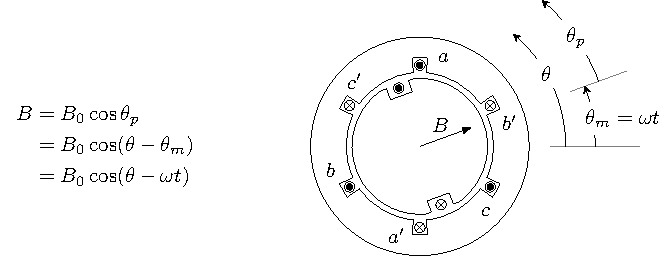
\includegraphics{figRotatingMachPrinciplesBasicACgenerator}
\begin{tikzpicture}
\stator{6}{30}
\slotDot{90,-30,210}
\slotCross{-90,30,150}
\pgfmathsetmacro{\pTheta}{150}
\pgfmathsetmacro{\pY}{0.2}
\pgfmathsetmacro{\rTilt}{20}
\rotor{2}{\rTilt}
%dot on rotot
\draw (90+\rTilt:\rR-\pX) circle (2.5pt);
\draw[fill] (90+\rTilt:\rR-\pX) circle (1.5pt);
%CROSS on rotor
\draw (\rTilt-90:\rR-\pX) circle (2.5pt);
\draw (\rTilt-90:\rR-\pX)++(45:2.2pt)--++(-135:4.4pt);
\draw (\rTilt-90:\rR-\pX)++(-45:2.2pt)--++(135:4.4pt);
%mmf vector and angles
\draw[-latex] (0,0)--(\rTilt:0.8*\rR)node[above,pos=0.4]{$B$};
\draw[gray](0:1.2*\sRo)--++(0:1.5cm);
\draw[gray](\rTilt:1.2*\sRo cm +0.5cm)--++(\rTilt:1cm);
%
\draw[-stealth] (0:1.2*\sRo cm +0.75 cm)  arc (0:\rTilt:1.2*\sRo cm +0.75 cm);
\draw node[right,fill=white] at (\rTilt/2:1.2*\sRo cm+0.5 cm){$\theta_m=\omega t$}; 
%
\draw[-stealth] (\rTilt:1.2*\sRo cm +1 cm)  arc (\rTilt:\rTilt+30:1.2*\sRo cm +1 cm);
\draw node[fill=white] at (\rTilt+15:1.2*\sRo+1){$\theta_p$};
%
\draw[-stealth] (0:1.2*\sRo cm +0.25 cm)  arc (0:\rTilt+30:1.2*\sRo cm +0.25 cm);
\draw node[fill=white] at (\rTilt/2+20:1.2*\sRo cm+0.25 cm){$\theta$};
%\slotName{45/a_1/,-45/a_1'/below,135/a_2'/,-135/a_2/below}
\draw (90-15:\sRi+1.25*\delR)node[]{$a$};
\draw (270-15:\sRi+1.25*\delR)node[]{$a'$};
\draw (210-15:\sRi+1.25*\delR)node[]{$b$};
\draw (30-15:\sRi+1.25*\delR)node[]{$b'$};
\draw (-30-15:\sRi+1.25*\delR)node[]{$c$};
\draw (150-15:\sRi+1.25*\delR)node[]{$c'$};
%text
\draw node[left] at (-1.5*\sRo,0){$
\begin{aligned}
B&=B_0 \cos \theta_p\\
&=B_0 \cos(\theta-\theta_m)\\
&=B_0 \cos (\theta-\omega t)
\end{aligned}
$};
\end{tikzpicture}%
\caption{بنیادی بدلتا رو جنریٹر۔}
\label{شکل_گھومتے_مشین_بنیادی_بدلتی_رو_جنریٹر}
\end{figure}%
%
\begin{align}
B=B_0 \cos \theta_p
\end{align}
یہ مقناطیس \عددیء{\omega}  زاویاتی رفتار سے گھوم رہا ہے۔ابتدائی لمحہ  \عددیء{t=0} پر  اس مقناطیس کو لچھا \عددیء{a} کے رخ، یعنی ہلکی سیاہی کی  افقی لکیر پر تصور کریں۔ یوں  لمحہ  \عددیء{t} پر یہ گھوم کر زاویہ \عددیء{\theta_m=\omega t} پر ہو گا۔اس طرح درج بالا مساوات  درج ذیل لکھی جا سکتی ہے۔
\begin{gather}
\begin{aligned}\label{مساوات_گھومتے_مشین_کثافت_بالمقابل_زاویہ}
B&=B_0 \cos (\theta-\theta_m)\\
&=B_0 \cos (\theta -\omega t)
\end{aligned}
\end{gather}
%
\begin{figure}
\centering
%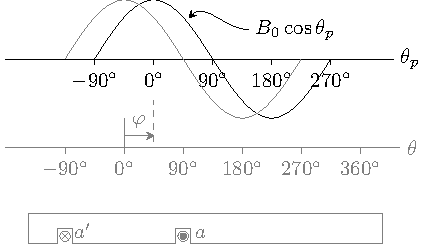
\includegraphics{figRotatingMachPrinciplesFluxCuttingSingleStatorCoil}
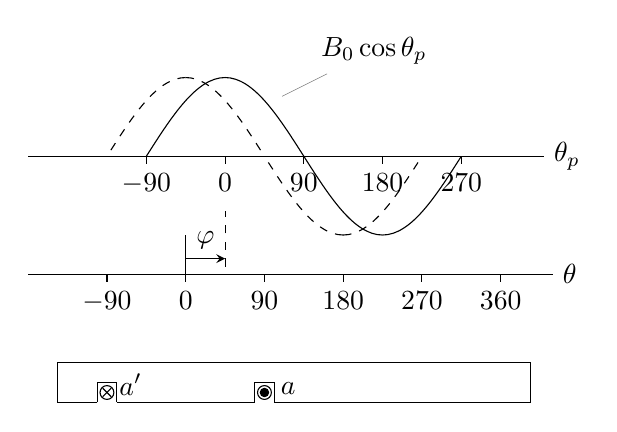
\begin{tikzpicture}
\pgfmathsetmacro{\shiftY}{2.5}
\begin{scope}[]
%\newcommand{\dotLinear}[1]{
\pgfmathsetmacro{\delSlotX}{3.5}
\foreach \x in {90}{
\pgfmathsetmacro{\x}{\x/90}
\draw(\x cm-\delSlotX pt,-\delSlotX pt)--++(0,2*\delSlotX pt)--++(2*\delSlotX pt,0)--++(0,-2*\delSlotX pt);
\draw (\x,0) circle (2.5pt);
\draw[fill] (\x,0) circle (1.5pt); }
\draw node[shift={(0.3,0.05)}] at (1,0){$a$};
%====================================
%CROSS LINEAR
%\crossLinear{comma separated x-locations}
\pgfmathsetmacro{\delSlotX}{3.5}
\foreach \x in {-90}{
\pgfmathsetmacro{\x}{\x/90}
\draw(\x cm-\delSlotX pt,-\delSlotX pt)--++(0,2*\delSlotX pt)--++(2*\delSlotX pt,0)--++(0,-2*\delSlotX pt);
\draw (\x,0) circle (2.5pt);
\draw (\x,0)++(45:2.2pt)--++(-135:4.4pt);
\draw (\x,0)++(-45:2.2pt)--++(135:4.4pt);  }
\draw node[shift={(0.3,0.1)}] at (-1,0){$a'$};
%==================================
%SLOT SEGMENT
%\slotSegment{comma separated xStart/xEnd locations}
\pgfmathsetmacro{\delSlotX}{3.5}
\foreach \xStart/\xEnd in {-90/90,90/360}{
\pgfmathsetmacro{\xStart}{\xStart/90}
\pgfmathsetmacro{\xEnd}{\xEnd/90}
\draw(\xStart cm+\delSlotX pt,-\delSlotX pt) --(\xEnd cm -\delSlotX pt,-\delSlotX pt); }
%
%this is used after \slotSegment to draw the top cover
%\newcommand{\slotTop}[1]{
\foreach \xStart/\xEnd in {-90/360}{
\pgfmathsetmacro{\xStart}{\xStart/90}
\pgfmathsetmacro{\xEnd}{\xEnd/90}
\draw (\xStart cm-\delSlotX pt,-\delSlotX pt)--++(-0.5 cm,0)--++(0,0.5)--++(\xEnd cm-\xStart cm+1 cm ,0)--++(0,-0.5)--(\xEnd cm-\delSlotX pt,-\delSlotX pt); }
%================================
%axis
\draw (-180/90, 1.5)--++(600/90,0)node[right]{$\theta$};
\draw(0,1.5)--++(0,0.5);
\foreach \x in {-90,0,90,180,270,360}{
\draw (\x/90,1.5)--++(0,-0.1)node[below]{$\x\degree$}; }
%
\draw[dashed](0.5,1.5+0.1)--++(0,0.7);
\draw[-stealth](0,1.5+0.2)--++(0.5,0)node[above,pos=0.5]{$\varphi$};
\end{scope}
%
\begin{scope}[xshift=0.5 cm,yshift=3 cm ]
%axis
\draw (-225/90, 0)--++(590/90,0)node[right]{$\theta_p$};
\foreach \x in {-90,0,90,180,270}{
\draw (\x/90,0)--++(0,-0.1)node[below]{$\x\degree$}; }
%cosine DARK
\draw[] (0,1) cos (-1,0);
\draw[] (0,1) cos (1,0);
\draw[](2,-1) cos (1,0);
\draw[] (2,-1) cos (3,0);
%cosine LIGHT
\draw[dashed](-0.5,1) cos (-1.5,0);
\draw[dashed] (-0.5,1) cos (0.5,0);
\draw[dashed](1.5,-1) cos (0.5,0);
\draw [dashed](1.5,-1) cos (2.5,0);
%text
\draw[] (0.6,0.7) node[pin=35:{$B_0 \cos \theta_p$}]{};
\end{scope}
\end{tikzpicture}%
\caption{لچھے میں سے گزرتا مقناطیسی بہاو۔}
\label{شکل_گھومتے_مشین_لچھے_سے_گزرتی_بیاو}
\end{figure}%
%
شکل \حوالہ{شکل_گھومتے_مشین_لچھے_سے_گزرتی_بیاو}  میں \عددیء{B} کو زاویہ \عددیء{\theta} اور \عددیء{\theta_p}  کے ساتھ ترسیم کیا گیا ہے اور ساتھ ہی  لچھا \عددیء{a} دکھایا گیا ہے۔لمحہ \عددیء{t=0}پر، جب  گھومتے برقی مقناطیس کا محور اور لچھا \عددی{a} کا محور ایک رخ  ہیں،  نقطہ دار  لکیر سے \عددیء{B} دکھایا گیا ہے جبکہ عمومی  لمحہ \عددیء{t} پر  \عددیء{B} کو  ٹھوس لکیر سے   دکھایا گیا ہے۔چونکہ \عددی{B} کی چوٹی ہر صورت \عددی{\theta_p=0\degree} پر ہو گی لہٰذا  ترسیم میں محور \عددی{\theta_p} پر دکھائے گئے زاویات \عددی{\-90\degree} تا \عددی{270\degree} عمومی لمحہ \عددی{t} کے لئے درست  ہیں نا کہ \عددی{t=0\degree} کے لئے۔لمحہ \عددی{t=0} پر \عددی{B} کی چوٹی عین \عددی{\theta=0\degree} پر ہو گی۔عمومی  لمحہ \عددی{t} پر برقی مقناطیس کے محور اور لچھے کے محور کے بیچ \عددیء{\vartheta} زاویہ ہے۔ یہ زاویہ برقی مقناطیس کے گھومنے کی رفتار \عددیء{\omega} پر منحصر ہو گا۔
\begin{align}
\vartheta=\omega t
\end{align}
لمحہ \عددیء{t=0} پر لچھا \عددی{a} میں   مقناطیسی بہاو زیادہ سے زیادہ ہو گا۔ خلائی درز باریک ہونے کی بنا درز کا اندرونی اور بیرونی رداس تقریباً  ایک دوسرے جیسا ہوں گے۔ برقی مقناطیس کے گھومنے کے محور سے  خلائی درز تک کا اوسط رداسی فاصلہ \عددیء{\rho} اور  برقی مقناطیس کی محوری لمبائی\فرہنگ{محوری!لمبائی}\حاشیہب{axial length} \عددیء{l} ہونے کی صورت میں لچھے میں  مقناطیسی بہاو وہی ہو گا جو  خلائی درز میں  \عددیء{-\tfrac{\pi}{2} < \theta < \tfrac{\pi}{2}}  کے بیچ ہے۔ لمحہ \عددیء{t=0} پر  لچھا \عددی{a} سے گزرتا بہاو  تلاش کرتے ہیں۔
\begin{gather}
\begin{aligned}\label{مساوات_گھومتے_مشین_قطب_پر_بہاو}
\phi_a(0)&=\int_{-\frac{\pi}{2}}^{+\frac{\pi}{2}} \kvec{B} \cdot \dif \kvec{S}\\
&=\int_{-\frac{\pi}{2}}^{+\frac{\pi}{2}} (B_0 \cos \theta_p)(l \rho \dif \theta_p)\\
&=B_0 l \rho \left. \sin \theta_p \right\vert_{-\frac{\pi}{2}}^{+\frac{\pi}{2}}\\
&=2 B_0 l \rho\\
&=\phi_0
\end{aligned}
\end{gather}
آخری قدم پر  \عددیء{\phi_a(0)} کو \عددیء{\phi_0} کہا گیا ہے۔ یہی حساب  لمحہ \عددیء{t} پر درج ذیل ہو گا جہاں آخری قدم پر \عددیء{\vartheta=\omega t} لیا گیا ہے۔
\begin{gather}
\begin{aligned}
\phi_a(t)&=\int_{-\frac{\pi}{2}-\vartheta}^{+\frac{\pi}{2}-\vartheta} \kvec{B} \cdot \dif \kvec{S}\\
&=\int_{-\frac{\pi}{2}-\vartheta}^{+\frac{\pi}{2}-\vartheta} (B_0 \cos \theta_p)(l \rho \dif \theta_p)\\
&=B_0 l \rho \left. \sin \theta_p \right\vert_{-\frac{\pi}{2}-\vartheta}^{+\frac{\pi}{2}-\vartheta}\\
&=2 B_0 l \rho \cos \vartheta\\
&=2 B_0 l \rho \cos \omega t
\end{aligned}
\end{gather}
اسی بہاو کو درج ذیل طریقہ سے بھی حاصل کیا جا سکتا ہے۔
\begin{gather}
\begin{aligned}\label{مساوات_گھومتے_مشین_قطبی_بہاو_بالمقابل_وقت}
\phi_a(t)&=\int_{-\frac{\pi}{2}}^{+\frac{\pi}{2}} \kvec{B} \cdot \dif \kvec{S}\\
&=\int_{-\frac{\pi}{2}}^{+\frac{\pi}{2}} (B_0 \cos (\theta-\omega t))(l \rho \dif \theta)\\
&=B_0 l \rho \left. \sin (\theta-\omega t) \right\vert_{-\frac{\pi}{2}}^{+\frac{\pi}{2}}\\
&=B_0 l \rho \left[\sin \left(\frac{\pi}{2}-\omega t \right )-\sin \left (-\frac{\pi}{2}-\omega t \right) \right]\\
&=2 B_0 l \rho \cos \omega t
\end{aligned}
\end{gather}
اس مرتبہ تکمل زاویہ \عددیء{\theta} کے ساتھ کیا گیا ہے۔ مساوات \حوالہ{مساوات_گھومتے_مشین_قطب_پر_بہاو}  کی مدد سے \عددی{\phi_a(t)}  کو درج ذیل لکھا جا سکتا ہے۔
\begin{align}
\phi_a(t)=2 B_0 l \rho \cos \omega t=\phi_0 \cos \omega t
\end{align}
مساوات  \حوالہ{مساوات_گھومتے_مشین_قطبی_بہاو_بالمقابل_وقت} کی طرح   \عددیء{b} اور \عددیء{c} لچھوں کے  مقناطیسی بہاو کی مساواتیں بھی حاصل کی جا سکتی ہیں۔شکل \حوالہ{شکل_گھومتے_مشین_بنیادی_بدلتی_رو_جنریٹر}  میں زاویہ \عددیء{-\tfrac{\pi}{2}} سے \عددیء{+\tfrac{\pi}{2}}  تک کا مقناطیسی بہاو لچھا \عددیء{a}  میں  گزرتا ہے۔ اس لئے \عددیء{\phi_a(t)}  معلوم کرنے کے لئے مساوات \حوالہ{مساوات_گھومتے_مشین_قطبی_بہاو_بالمقابل_وقت}  میں تکمل کے حد یہی رکھے گئے تھے۔یوں لچھا \عددیء{b}  کے تکمل کے حد  \عددیء{+\tfrac{\pi}{6}}  اور \عددیء{+\tfrac{7 \pi}{6}} جبکہ \عددیء{c} کے حد \عددیء{+\tfrac{5\pi}{6}} اور \عددیء{+\tfrac{11\pi}{6}} ہوں گے۔تمام زاویات ریڈیئن میں دیے گئے ہیں۔یوں درج ذیل ہو گا۔
\begin{gather}
\begin{aligned}
\phi_b(t)&=\int_{\frac{\pi}{6}}^{\frac{7\pi}{6}} \kvec{B} \cdot \dif \kvec{S}\\
&=\int_{\frac{\pi}{6}}^{\frac{7\pi}{6}} (B_0 \cos (\theta-\omega t))(l \rho \dif \theta)\\
&=B_0 l \rho \left. \sin (\theta-\omega t) \right\vert_{\frac{\pi}{6}}^{\frac{7\pi}{6}}\\
&=B_0 l \rho \left[\sin \left(\frac{7\pi}{6}-\omega t \right )-\sin \left (\frac{\pi}{6}-\omega t \right) \right]\\
&=2 B_0 l \rho \cos \big(\omega t-\frac{2\pi}{3}\big)
\end{aligned}
\end{gather}
اور
\begin{gather}
\begin{aligned}
\phi_c(t)&=\int_{\frac{5\pi}{6}}^{\frac{11\pi}{6}} \kvec{B} \cdot \dif \kvec{S}\\
&=\int_{\frac{5\pi}{6}}^{\frac{11\pi}{6}} (B_0 \cos (\theta-\omega t))(l \rho \dif \theta)\\
&=B_0 l \rho \left. \sin (\theta-\omega t) \right\vert_{\frac{5\pi}{6}}^{\frac{11\pi}{6}}\\
&=B_0 l \rho \left[\sin \left(\frac{11\pi}{6}-\omega t \right )-\sin \left (\frac{5\pi}{6}-\omega t \right) \right]\\
&=2 B_0 l \rho \cos \big(\omega t+\frac{2\pi}{3}\big)
\end{aligned}
\end{gather}
ایک لچھا کے \عددیء{N} چکر تصور کرتے ہوئے تینوں لچھوں میں پیدا برقی دباو معلوم کرتے ہیں۔لچھوں میں ارتباط بہاو درج ذیل ہو گا۔
\begin{gather}
\begin{aligned}
\lambda_a&=N \phi_a (t)=N \phi_0 \cos \omega t\\
\lambda_b&=N \phi_b (t)=N \phi_0 \cos (\omega t-120\degree)\\
\lambda_c&=N \phi_c (t)=N \phi_0 \cos (\omega t+120\degree)
\end{aligned}
\end{gather}
ان مساوات میں \عددیء{\tfrac{2\pi}{3}} ریڈیئن کو \عددیء{120\degree} لکھا گیا ہے۔ لچھوں میں پیدا امالی برقی دباو درج ذیل ہو گا۔
\begin{gather}
\begin{aligned}\label{مساوات_گھومتے_مشین_تین_دور_سائن_نما_برقی_دباو_الف}
e_a(t)&=\frac{\dif \lambda_a}{\dif t}=-\omega N \phi_0 \sin \omega t\\
e_b(t)&=\frac{\dif \lambda_b}{\dif t}=-\omega N \phi_0 \sin (\omega t-120\degree)\\
e_c(t)&=\frac{\dif \lambda_c}{\dif t}=-\omega N \phi_0 \sin (\omega t+120\degree)
\end{aligned}
\end{gather}
ان مساوات کو 
\begin{gather}
\begin{aligned}\label{مساوات_گھومتے_مشین_تین_دور_سائن_نما_برقی_دباو}
e_a(t)&=\omega N \phi_0 \cos (\omega t +90\degree)\\
e_b(t)&=\omega N \phi_0 \cos (\omega t-30\degree)\\
e_c(t)&=\omega N \phi_0 \cos (\omega t+210\degree)
\end{aligned}
\end{gather}
لکھا جا سکتا ہے جو آپس میں \عددیء{120\degree} زاویہ پر تین دوری محرک برقی دباو  کو ظاہر کرتی ہیں۔ ان سب کے حیطے \عددیء{E_0} ایک دوسرے جتنے ہیں
\begin{align}
E_0=\omega N \phi_0
\end{align}
لہٰذا  تینوں  برقی دباو کی موثر قیمت\فرہنگ{موثر قیمت}\حاشیہب{rms}\فرہنگ{rms} درج ذیل ہو گی۔
\begin{align}\label{مساوات_گھومتے_مشین_موثر_دباو}
E_{\textup{موثر}}=\frac{E_0}{\sqrt{2}}=\frac{2\pi f N \phi_0}{\sqrt{2}}=4.44 f N \phi_0
\end{align}
چونکہ \عددیء{\phi=B A} ہوتا ہے لہٰذا مساوات \حوالہ{مساوات_گھومتے_مشین_موثر_دباو}  صفحہ \حوالہصفحہ{مساوات_مقناطیسی_دور_پیدا_دباو_موثر_قیمت} پر دی گئی  مساوات \حوالہ{مساوات_مقناطیسی_دور_پیدا_دباو_موثر_قیمت}  کی طرح ہے۔ 

مساوات \حوالہ{مساوات_گھومتے_مشین_تین_دور_سائن_نما_برقی_دباو}  سائن نما برقی دباو کو ظاہر کرتی ہے۔ اگرچہ اسے  یہ تصور کر کے حاصل کیا گیا کہ خلائی درز میں مقناطیسی بہاو صرف برقی مقناطیس کی وجہ سے ہے تاہم برقی دباو کا اس سے کوئی تعلق نہیں کہ خلائی درز میں مقناطیسی بہاو کس طرح وجود میں آیا اور یہ مساوات ان حالات کے لئے بھی درست ہے جہاں خلائی درز میں مقناطیسی بہاو جنریٹر کے ساکن حصہ میں پیدا ہوئی ہو یا ساکن اور حرکت پذیر دونوں حصوں میں پیدا ہوئی ہو۔

مساوات \حوالہ{مساوات_گھومتے_مشین_موثر_دباو}  ہمیں ایک گچھ لچھے میں پیدا برقی دباو دیتی ہے۔ اگر لچھا تقسیم شدہ ہو تب اس کے مختلف شگافوں میں موجود اس لچھے کے حصوں میں برقی دباو ہم قدم نہیں ہوں گے لہٰذا ان سب کا مجموعی برقی دباو ان سب کا حاصل جمع نہیں ہو گا بلکہ اس سے کچھ  کم ہو گا۔ یوں پھیلے لچھے کے لئے  یہ مساوات  درج ذیل صورت اختیار کرتی ہے۔
\begin{align}
E_{\textup{موثر}} =4.44 k_w f N \phi_0
\end{align}
تین دوری برقی جنریٹروں کے \عددیء{k_w} کی قیمت \عددیء{0.85} تا \عددیء{0.95} ہوتی ہے۔ یہ مساوات ہمیں یک دوری برقی دباو دیتی ہے۔ تین دوری برقی جنریٹروں میں ایسے تین لچھوں کے جوڑے ہوتے ہیں اور ان کو \عددیء{Y} یعنی ستارہ  یا \عددیء{\Delta} یعنی تکونی جوڑا جاتا ہے۔


\جزوحصہ{یک سمت رو برقی جنریٹر}
ہر گھومنے والا برقی جنریٹر بنیادی طور پر بدلتا رو جنریٹر ہوتا ہے۔ البتہ جہاں یک سمت برقی دباو\فرہنگ{برقی دباو!یک سمت}\حاشیہب{DC voltage}\فرہنگ{voltage!DC}  کی ضرورت ہو وہاں مختلف طریقوں سے بدلتا برقی دباو  کو یک سمت برقی دباو میں تبدیل کیا جاتا ہے۔   جنریٹر کے باہر \اصطلاح{برقیاتی سمت کار}\فرہنگ{سمت کار!برقیاتی}\حاشیہب{rectifier}\فرہنگ{rectifier}  یا جنریٹر کے اندر  \اصطلاح{میکانی سمت کار}\فرہنگ{سمت کار!میکانی}\حاشیہب{commutator}\فرہنگ{commutator}  نسب کر کے بدلتا دباو سے یک سمت دباو حاصل کیا جا سکتا ہے۔ مساوات \حوالہ{مساوات_گھومتے_مشین_تین_دور_سائن_نما_برقی_دباو_الف}  کے \عددی{e_a}   کو یک سمت برقی دباو میں تبدیل کرنے سے  شکل \حوالہ{شکل_گھومتے_مشین_ایک_دور_یک_سمتی_برقی_دباو}  حاصل ہو گا۔
\begin{figure}
\centering
%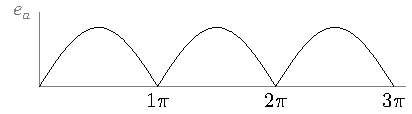
\includegraphics{figRotatingMachPrinciplesFullWaveDCvoltage}
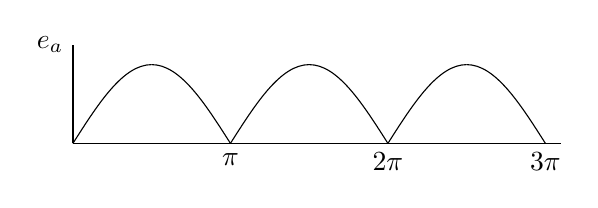
\begin{tikzpicture}
%axis
\draw[] (0,0)--(6.2,0);
\draw[](0,0)--(0,1.25) node[left]{$e_a$};
%cosine DARK
\draw (1,1) cos (0,0);
\draw (1,1) cos (2,0);
\draw (3,1) cos (2,0);
\draw(3,1) cos (4,0);
\draw (5,1) cos (4,0);
\draw (5,1) cos (6,0);
\draw node[below] at (2,0){$\pi$};
\draw node[below] at (4,0){$2\pi$};
\draw node[below] at (6,0){$3\pi$};
\end{tikzpicture}
\caption{یک دوری یک سمت برقی دباو۔}
\label{شکل_گھومتے_مشین_ایک_دور_یک_سمتی_برقی_دباو}
\end{figure}
\ابتدا{مثال}
شکل \حوالہ{شکل_گھومتے_مشین_ایک_دور_یک_سمتی_برقی_دباو}  میں یک سمت برقی دباو دکھایا گیا ہے۔اس یک سمت برقی دباو کی اوسط قیمت حاصل کریں۔

حل:
\begin{align*}
E_{\textup{اوسط}}=\frac{1}{\pi} \int_{0}^{\pi} \omega N \phi_0 \sin \omega t \dif \,(\omega t)=\frac{2 \omega N \phi_0}{\pi}
\end{align*}
\انتہا{مثال}

یک سمت جنریٹر پر  باب  \حوالہ{باب_یک_سمتی_رو_مشین} میں غور کیا جائے گا۔

\حصہ{ہموار قطب مشینوں میں قوت مروڑ}
اس حصہ میں  کامل مشین میں \اصطلاح{قوت مروڑ}\فرہنگ{قوت مروڑ}\حاشیہب{torque}\فرہنگ{torque} کے حصول کے دو تراکیب پر غور کیا جائے گا۔ ایک ترکیب میں مشین کو دو مقناطیس تصور کر کے  ان  مقناطیسوں کے بیچ قوت کشش، قوت دفع اور قوت مروڑ حاصل کیے جائیں گے  جبکہ دوسری ترکیب  میں  مشین کے ساکن اور گھومتے لچھوں کو امالہ تصور کر کے  (باب چار کی طرح)  توانائی اور ہم-توانائی سے ان کا حساب لگایا جائے گا۔ پہلے توانائی کی ترکیب پر غور کرتے ہیں۔

\جزوحصہ{میکانی قوت مروڑ بذریعہ ترکیب توانائی}
یہاں یک دوری مشین  پر غور کیا جائے گا جس سے  حاصل نتائج  با آسانی زیادہ دور کی مشینوں  پر لاگو کیے جا سکتے ہیں۔ شکل \حوالہ{شکل_گھومتے_مشین_ساکن_گھومتا_امالہ} میں یک دوری  کامل مشین دکھائی گئی ہے۔ کسی بھی لمحہ اس مشین کے دو لچھوں کے بیچ  کوئی زاویہ ہو گا جسے \عددیء{\theta} سے ظاہر کیا گیا ہے۔ خلائی درز ہر مقام پر یکساں ہے لہٰذا ابھرے قطب کے اثرات کو نظر انداز کیا جاتا ہے۔ مزید قالب کا جزو مقناطیس مستقل لامتناہی  (\عددیء{\mu_r \to \infty})  تصور کیا گیا ہے لہٰذا لچھوں کا امالہ صرف خلائی درز کے مقناطیسی مستقل\فرہنگ{مقناطیسی مستقل}\حاشیہب{magnetic constant, permeability} \عددیء{\mu_0} پر منحصر ہو گا۔
\begin{figure}
\centering
%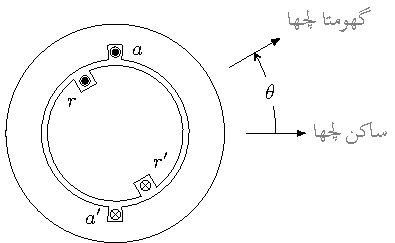
\includegraphics{figRotatingMachPrinciplesStatorAndRotorInductances}
\begin{tikzpicture}
\stator{2}{90}
\slotDot{90}
\slotCross{270}
\draw node at (90-15:\sRi+2*\gap){$a$};
\draw node at (-90-15:\sRi+2*\gap){$a'$};
%ROTOR
\pgfmathsetmacro{\pTheta}{165}
\pgfmathsetmacro{\pX}{0}
\pgfmathsetmacro{\pY}{0.25}
\pgfmathsetmacro{\rTilt}{30}
\rotor{2}{\rTilt}
%rotor dot
\draw (\rTilt+90:\rR-\delR/2) circle (2.5pt);
\draw[fill] (\rTilt+90:\rR-\delR/2) circle (1.5pt); 
%rotor cross
\draw (\rTilt-90:\rR-\delR/2) circle (2.5pt);
\draw (\rTilt-90:\rR-\delR/2)++(45:2.2pt)--++(-135:4.4pt);
\draw (\rTilt-90:\rR-\delR/2)++(-45:2.2pt)--++(135:4.4pt); 
%text
\draw node at (\rTilt+90+25:\rR-\pY){$r$};
\draw node at (\rTilt-90+30:\rR-\pY){$r'$};
%urdu
\draw[-latex] (0:1.2*\sRo)--++(0:1cm)node[right]{\RL{ساکن لچھا}};
\draw[-latex] (\rTilt:1.2*\sRo)--++(\rTilt:1cm)node[above right]{\RL{گھومتا لچھا}};
\draw[-stealth] (0:1.2*\sRo cm+0.5 cm) arc (0:\rTilt:1.2*\sRo cm+0.5 cm);
\draw  node[fill=white] at (\rTilt/2:1.2*\sRo cm+0.5 cm){$\theta$};
\end{tikzpicture}
\caption{ساکن امالہ اور گھومتا امالہ۔}
\label{شکل_گھومتے_مشین_ساکن_گھومتا_امالہ}
\end{figure}

اس طرح ساکن لچھے کا امالہ \عددیء{L_{aa}} اور گھومے لچھے کا امالہ \عددیء{L_{rr}} مستقل ہوں گے جبکہ ان کا مشترکہ امالہ \عددیء{L_{ar}(\theta)} زاویہ \عددیء{\theta} پر منحصر ہو گا۔ جس لمحہ \عددیء{\theta=0} یا \عددیء{\theta=\mp 2\pi} ہو اس لمحہ  ایک لچھے کا سارا مقناطیسی بہاو دوسرے لچھے سے بھی گزرتا ہے اور ان کا مشترکہ امالہ زیادہ سے زیادہ ہو گا جسے \عددیء{L_{ar0}} سے ظاہر کیا جائے گا۔ جس لمحہ  \عددیء{\theta=\mp 180\degree} ہو اس لمحہ دوبارہ ایک لچھے کا سارا مقناطیسی بہاو دوسرے لچھے سے بھی گزرتا ہے لیکن اس بار اس کا رخ الٹ ہوتا ہے  لہٰذا ا ان کا مشترکہ امالہ منفی ہو گا، \عددیء{-L_{ar0}}،  جبکہ  \عددیء{\theta=\mp 90\degree} پر  ان کا مشترکہ امالہ صفر ہو گا۔خلائی درز میں  مقناطیسی بہاو سائن نما
\begin{align}
L_{ar}=L_{ar0} \cos \theta
\end{align}
تصور کرتے ہوئے  ساکن اور گھومتے لچھوں کے ارتباط بہاو درج ذیل ہوں گے۔
\begin{gather}
\begin{aligned}
\lambda_a&=L_{aa} i_a+L_{ar}(\theta) i_r=L_{aa} i_a+L_{ar0} \cos (\theta) i_r\\
\lambda_r&=L_{ar}(\theta) i_a+L_{rr} i_r=L_{ar0} \cos (\theta) i_a+L_{rr} i_r
\end{aligned}
\end{gather}
ساکن لچھے کی مزاحمت \عددیء{R_a} اور گھومتے لچھے کی مزاحمت \عددیء{R_r} لیتے ہوئے ان لچھوں کے سروں پر  قانون کرخوف سے برقی دباو درج ذیل ہوں گے۔
\begin{gather}
\begin{aligned}
v_a&=i_a R_a +\frac{\dif \lambda_a}{\dif t}=i_a R_a+L_{aa} \frac{\dif i_a}{\dif t}+L_{ar0} \cos \theta \frac{\dif i_r}{\dif t}-L_{ar0}  i_r \sin \theta  \frac{\dif \theta}{\dif t}\\
v_r&=i_r R_r +\frac{\dif \lambda_r}{\dif t}=i_r R_r+L_{ar0} \cos \theta \frac{\dif i_a}{\dif t}-L_{ar0} i_a \sin \theta  \frac{\dif \theta}{\dif t}+L_{rr} \frac{\dif i_r}{\dif t}
\end{aligned}
\end{gather}
یہاں \عددیء{\theta} برقی زاویہ ہے جس کی وقت کے ساتھ  تبدیلی،   \عددیء{\omega} دے گی۔
\begin{align}
\frac{\dif \theta}{\dif t}=\omega
\end{align}
میکانی قوت مروڑ بذریعہ ہم-توانائی حاصل کی جا سکتی ہے۔ ہم-توانائی صفحہ \حوالہصفحہ{مساوات_تبادلہ_کوتوانائی_از_خود} پر مساوات \حوالہ{مساوات_تبادلہ_کوتوانائی_از_خود}  سے حاصل ہو گی۔یہ مساوات موجودہ استعمال کے لئے درج ذیل صورت اختیار کرتی ہے۔
\begin{align}
W_m'=\frac{1}{2} L_{aa} i_a^2+\frac{1}{2} L_{rr} i_r^2+L_{ar0} i_a i_r \cos \theta
\end{align}
اس سے میکانی قوت مروڑ \عددیء{T_m} حاصل کرتے ہیں۔
\begin{align}\label{مساوات_گھومتے_مشین_مروڑ_بذریعہ_توانائی}
T_m=\frac{\partial W_m'(\theta_m,i_a,i_r)}{\partial \theta_m}=\frac{\partial W_m'(\theta,i_a,i_r)}{\partial \theta} \frac{\partial \theta}{\partial \theta_m}
\end{align}
چونکہ \عددیء{P} قطب مشینوں کے لئے درج ذیل ہوتا ہے
\begin{align}
\theta=\frac{P}{2} \theta_m
\end{align}
لہٰذا ہمیں مساوات \حوالہ{مساوات_گھومتے_مشین_مروڑ_بذریعہ_توانائی}  سے درج ذیل حاصل ہو گا۔
\begin{align}\label{مساوات_گھومتے_مشین_مروڑ_بذریعہ_کوتوانائی}
T_m=-\frac{P}{2} L_{ar0} i_a i_r \sin \left(\frac{P}{2} \theta_m\right)
\end{align}
اس مساوات میں قوت مروڑ \عددیء{T_m} کی علامت منفی ہے۔ یوں جس لمحہ پر ساکن اور گھومتے لچھوں کے مقناطیسی بہاو کے بیچ  زاویہ مثبت ہو، اس لمحہ پر ان لچھوں کے بیچ قوت مروڑ منفی ہو گا۔  قوت مروڑ  دونوں مقناطیسی بہاو کو ایک رخ میں رکھنے کی کوشش کرتا ہے۔

\جزوحصہ{میکانی قوت مروڑ بذریعہ مقناطیسی بہاو}
شکل \حوالہ{شکل_گھومتے_مشین_لچھوں_کی_قطبین}-ا  میں دو قطبی یک دوری مشین کے صرف گھومتے لچھے میں برقی رو پایا جاتا ہے۔   مشین کا  گھومتا حصہ  ایک مقناطیس کی مانند ہے جس کے شمالی اور جنوبی قطبین دکھائے گئے ہیں۔ اس لچھے کا مقناطیسی بہاو تیر کے نشان سے دکھایا گیا ہے لہٰذا  تیر اس مقناطیس کے محور کو ظاہر کرتا ہے۔

شکل \حوالہ{شکل_گھومتے_مشین_لچھوں_کی_قطبین}-ب میں  صرف ساکن لچھے میں برقی رو پایا جاتا ہے۔ ساکن حصہ سے مقناطیسی بہاو خارج ہو کر خلائی درز سے ہوتا ہوا گھومتے حصہ میں داخل ہوتا ہے لہٰذا یہی اس کا شمالی قطب ہو گا۔یہاں ساکن حصہ ایک مقناطیس مانند ہے جس کا محور  تیر سے ظاہر کیا گیا ہے۔
\begin{figure}
\centering
%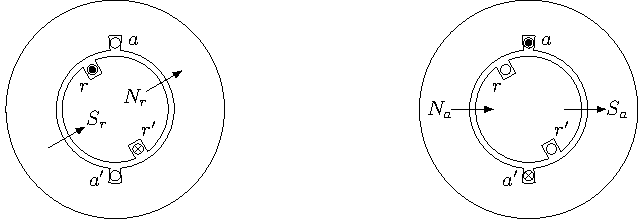
\includegraphics{figRotatingMachPrinciplesStatorAndRotorMagneticPoles}
\begin{subfigure}{0.45\textwidth}
\centering
\begin{tikzpicture}
\stator{2}{90}
\slotEmptyCircle{90}
\slotEmptyCircle{270}
\draw node at (90-15:\sRi+2*\gap){$a$};
\draw node at (-90-15:\sRi+2*\gap){$a'$};
%
%ROTOR
\pgfmathsetmacro{\pTheta}{165}
\pgfmathsetmacro{\pX}{0}
\pgfmathsetmacro{\pY}{0.25}
\pgfmathsetmacro{\rTilt}{30}
\rotor{2}{\rTilt}
%rotor dot
\draw (\rTilt+90:\rR-\delR/2) circle (2.5pt);
\draw[fill] (\rTilt+90:\rR-\delR/2) circle (1.5pt); 
%rotor cross
\draw (\rTilt-90:\rR-\delR/2) circle (2.5pt);
\draw (\rTilt-90:\rR-\delR/2)++(45:2.2pt)--++(-135:4.4pt);
\draw (\rTilt-90:\rR-\delR/2)++(-45:2.2pt)--++(135:4.4pt); 
%
\draw[-latex] (\rTilt:\rR cm-0.3 cm)node[shift={(180+\rTilt:0.2cm)}]{$N_r$}--++(\rTilt:0.7cm);
\draw[latex-] (180+\rTilt:\rR cm-0.3 cm)node[shift={(\rTilt:0.25cm)}]{$S_r$}--++(180+\rTilt:0.7cm);
%text)
\draw node at (\rTilt+90+25:\rR-\pY){$r$};
\draw node at (\rTilt-90+30:\rR-\pY){$r'$};
\end{tikzpicture}
\caption{}
\end{subfigure}%
\begin{subfigure}{0.45\textwidth}
\centering
\begin{tikzpicture}
\pgfmathsetmacro{\sRi}{0.8*\sRi}
\pgfmathsetmacro{\rR}{\sRi-\gap}
\stator{2}{90}
\slotDot{90}
\slotCross{270}
\draw node at (90-15:\sRi+2*\gap){$a$};
\draw node at (-90-15:\sRi+2*\gap){$a'$};
%
\draw[-latex] (0:\rR cm-0.3 cm)--++(0:0.7cm)node[xshift=0.2cm]{$S_a$};
\draw[latex-] (180:\rR cm-0.3 cm)--++(180:0.7cm)node[xshift=-0.2cm]{$N_a$};
%ROTOR
\pgfmathsetmacro{\pTheta}{165}
\pgfmathsetmacro{\pX}{0}
\pgfmathsetmacro{\pY}{0.25}
\pgfmathsetmacro{\rTilt}{30}
\rotor{2}{\rTilt}
%rotor no current
\draw (\rTilt+90:\rR-\delR/2) circle (2.5pt);
\draw (\rTilt-90:\rR-\delR/2) circle (2.5pt);
%text
\draw node at (\rTilt+90+25:\rR-\pY){$r$};
\draw node at (\rTilt-90+30:\rR-\pY){$r'$};
\end{tikzpicture}
\caption{}
\end{subfigure}%
\caption{لچھوں کے قطبین۔}
\label{شکل_گھومتے_مشین_لچھوں_کی_قطبین}
\end{figure}

اگرچہ شکل \حوالہ{شکل_گھومتے_مشین_لچھوں_کی_قطبین} میں  گچھ لچھے دکھائے گئے ہیں،  درحقیقت دونوں لچھوں کے مقناطیسی دباو سائن-نما  ہیں اور تیر کے نشان ان مقناطیسی دباو کی امواج کی چوٹیوں کو ظاہر کرتے ہیں۔

شکل \حوالہ{شکل_گھومتے_مشین_خلائی_درز_مجموعی_دباو}  میں دونوں لچھوں کو برقی رو فراہم کی گئی  ہے۔ دونوں لچھوں کے مخالف قطبین کے بیچ قوت کشش پایا جائے  گا جس کی بنا دونوں لچھے ایک ہی رخ ہونے کی کوشش کریں گے۔
\begin{figure}
\centering
%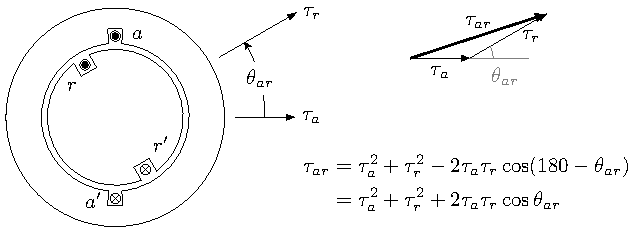
\includegraphics{figRotatingMachPrinciplesCombinedStatorAndRotorMMF}
\begin{tikzpicture}
\stator{2}{90}
\slotDot{90}
\slotCross{270}
\draw node at (90-15:\sRi+2*\gap){$a$};
\draw node at (-90-15:\sRi+2*\gap){$a'$};
%
%ROTOR
\pgfmathsetmacro{\pTheta}{165}
\pgfmathsetmacro{\pX}{0}
\pgfmathsetmacro{\pY}{0.25}
\pgfmathsetmacro{\rTilt}{30}
\rotor{2}{\rTilt}
%rotor dot
\draw (\rTilt+90:\rR-\delR/2) circle (2.5pt);
\draw[fill] (\rTilt+90:\rR-\delR/2) circle (1.5pt); 
%rotor cross
\draw (\rTilt-90:\rR-\delR/2) circle (2.5pt);
\draw (\rTilt-90:\rR-\delR/2)++(45:2.2pt)--++(-135:4.4pt);
\draw (\rTilt-90:\rR-\delR/2)++(-45:2.2pt)--++(135:4.4pt); 
%text
\draw node at (\rTilt+90+25:\rR-\pY){$r$};
\draw node at (\rTilt-90+30:\rR-\pY){$r'$};
%
\draw[-latex](0:1.1*\sRo)--++(0:1cm)node[right]{$\tau_a$};
\draw[-latex](\rTilt:1.1*\sRo)--++(\rTilt:1.5cm)node[right]{$\tau_r$};
\draw[-stealth] (0:1.1*\sRo cm+0.5cm) arc (0:\rTilt:1.1*\sRo cm +0.5 cm);
\draw node[fill=white] at (\rTilt/2:1.1*\sRo cm+0.5 cm){$\theta_{ar}$};
%text
\draw (3 cm,-0.5 cm) node[below right] {$
\begin{aligned}
\tau_{ar}&=\tau_a^2+\tau_r^2-2 \tau_a \tau_r \cos (180-\theta_{ar})\\
&=\tau_a^2+\tau_r^2+2 \tau_a \tau_r \cos \theta_{ar}
\end{aligned}
$};
%
\begin{scope}[xshift=5 cm,yshift=1cm]
\draw[-latex] (0,0)--++(0:1 cm)coordinate(aTip)node[below,pos=0.5]{$\tau_a$};
\draw[-latex] (aTip)--++(\rTilt:1.5 cm)coordinate(rTip)node[below,pos=0.8]{$\tau_r$};
\draw[-latex,thick](0,0)--(rTip)node[above,pos=0.5]{$\tau_{ar}$};
%angle
\draw[](aTip)--++(1cm,0);
\draw[](aTip)++(0.4cm,0)node[shift={(0.2cm,-0.3cm)}]{$\theta_{ar}$} arc (0:\rTilt:0.4 cm);
\end{scope}
\end{tikzpicture}
\caption{خلائی درز میں مجموعی مقناطیسی دباو۔}
\label{شکل_گھومتے_مشین_خلائی_درز_مجموعی_دباو}
\end{figure}

واضح رہے کہ  دونوں لچھے (مقناطیس) کوشش کریں گے کہ \عددیء{\theta_{ar}} صفر کے برابر ہو یعنی ان کا میکانی قوت مروڑ  \عددیء{\theta_{ar}} کے مخالف رخ ہو گا۔ یہی مساوات \حوالہ{مساوات_گھومتے_مشین_مروڑ_بذریعہ_کوتوانائی}  کہتی  ہے ۔

لچھوں  کے مقناطیسی دباو کو  مقناطیسی محور کے رخ  \عددیء{\سمتیہ{\tau}_a} اور \عددیء{\سمتیہ{\tau}_r} سے ظاہر کیا گیا ہے  جہاں \عددیء{\tau_a} اور \عددیء{\tau_r} سائن نما مقناطیسی دباو کی چوٹیوں کے برابر ہیں۔   خلائی درز میں کل مقناطیسی دباو \عددیء{\سمتیہ{\tau}_{ar}} ان  کا مجموعہ ہو گا جس کا طول \عددیء{\tau_{ar}} کلیہ کوسائن \حاشیہب{cosine law}  سے حاصل ہو گا:
\begin{gather}
\begin{aligned}\label{مساوات_گھومتے_مشین_مربع_کل_دباو}
\tau_{ar}^2&=\tau_a^2+\tau_r^2-2\tau_a \tau_r \cos (180\degree-\theta_{ar})\\
&=\tau_a^2+\tau_r^2+2\tau_a \tau_r \cos \theta_{ar}
\end{aligned}
\end{gather}
خلائی درز میں کل مقناطیسی دباو \عددی{\tau_{ar}} درج ذیل مقناطیسی شدت \عددیء{H_{ar}} پیدا کرے گا جہاں \عددی{l_g} کلائی درز کی لمبائی ہے۔
\begin{align}
\tau_{ar}=H_{ar} l_g
\end{align}

\عددیء{H_{ar}} مقناطیسی شدت کی چوٹی کو ظاہر کرتا ہے۔  خلاء میں جس مقام پر مقناطیسی شدت \عددیء{H} ہو وہاں مقناطیسی ہم-توانائی کی کثافت \عددیء{\tfrac{\mu_0}{2}H^2} ہوتی ہے۔ خلائی درز میں اوسط ہم-توانائی کی کثافت،  درز میں \عددیء{H^2} کی اوسط کو \عددیء{\tfrac{\mu_0}{2}} سے ضرب کر کے حاصل ہو گا۔ کسی بھی سائن نما موج \عددیء{H=H_0 \cos \theta} کے \عددیء{H^2} کا اوسط \عددیء{H_{\textup{اوسط}}^2}  حاصل کرتے ہیں:
\begin{gather}
\begin{aligned}
H_{\textup{اوسط}}^2&=\frac{1}{\pi} \int_{-\frac{\pi}{2}}^{+\frac{\pi}{2}} H^2 \dif \theta\\
&=\frac{1}{\pi} \int_{-\frac{\pi}{2}}^{+\frac{\pi}{2}} H_0^2 \cos^2 \theta \dif \theta\\
&=\frac{H_0^2}{\pi} \int_{-\frac{\pi}{2}}^{+\frac{\pi}{2}} \frac{1+\cos 2 \theta}{2} \dif \theta\\
&=\frac{H_0^2}{\pi}  \left.  \frac{\theta +\frac{\sin 2 \theta}{2}}{2} \right|_{-\frac{\pi}{2}}^{+\frac{\pi}{2}}\\
&=\frac{H_0^2}{2}
\end{aligned}
\end{gather}
یوں خلائی درز میں اوسط ہم-توانائی کی کثافت \عددیء{\tfrac{\mu_0}{2}\tfrac{H_{ar}^2}{2}} ہو گی۔ خلائی درز میں اوسط ہم-توانائی کو خلاء کے حجم سے ضرب کر کے درز میں  کل ہم-توانائی \عددی{W_m'}  حاصل ہو گی:
\begin{align}
W_m'=\frac{\mu_0}{2} \frac{H_{ar}^2}{2} 2 \pi r l_g l=\frac{\mu_0 \pi r l}{2l_g} \tau_{ar}^2
\end{align}
اس مساوات میں خلائی درز کی رداسی لمبائی \عددیء{l_g}  اور دھرے\حاشیہب{axis} کے رخ محوری لمبائی\حاشیہب{axial length} \عددیء{l} ہے۔ محور سے خلائی درز  کا اوسط رداسی فاصلہ \عددیء{r} ہے۔ مزید \عددیء{r\gg l_g} تصور کیا گیا ہے جس کی بنا درز میں رداسی رخ،  کثافت مقناطیسی بہاو کی تبدیلی  نظر انداز کی جا سکتی ہے۔ اس مساوات کو ہم مساوات \حوالہ{مساوات_گھومتے_مشین_مربع_کل_دباو}  کی مدد سے درج ذیل لکھ سکتے ہیں۔
\begin{align}
W_m'=\frac{\mu_0 \pi r l}{2 l_g} \left(\tau_a^2+\tau_r^2+2\tau_a \tau_r \cos \theta_{ar} \right) 
\end{align}
یوں میکانی قوت مروڑ درج ذیل ہو گا۔
\begin{align}\label{مساوات_گھومتے_مشین_مروڑ_کوتوانائی_سے}
T_m=\frac{\partial W_m'}{\partial \theta_{ar}}=-\frac{\mu_0 \pi r l}{l_g} \tau_a \tau_r \sin \theta_{ar}
\end{align}
مساوات \حوالہ{مساوات_گھومتے_مشین_مروڑ_کوتوانائی_سے} میں قوت مروڑ  دو قطبی مشین کے لئے حاصل کی گئی۔\عددیء{P} قطبی مشین کے لئے یہ مساوات ہر جوڑی قطب کی میکانی قوت مروڑ دیتی ہے لہٰذا \عددی{P} قطبی مشین کی قوت مروڑ \عددی{\tfrac{P}{2}} گنّا ہو گی:
\begin{align}\label{مساوات_گھومتے_مشین_مروڑ_بذریعہ_کوتوانائی_الف}
T_m=-\frac{P}{2}\frac{\mu_0 \pi r l}{l_g} \tau_a \tau_r \sin \theta_{ar}
\end{align}
مساوات \حوالہ{مساوات_گھومتے_مشین_مروڑ_بذریعہ_کوتوانائی_الف} ایک اہم مساوات ہے جس کے مطابق مشین کی میکانی قوت مروڑ، ساکن اور گھومتے لچھوں کے مقناطیسی دباو کی چوٹیوں اور  دونوں کے بیچ برقی زاویہ \عددیء{\theta_{ar}} کے سائن کی  راست متناسب ہو گی۔ منفی میکانی قوت مروڑ کا مطلب ہے کہ یہ زاویہ  \عددیء{\theta_{ar}} کے مخالف رخ ہو گی یعنی میکانی قوت مروڑ اس زاویہ کو کم کرنے کی کوشش کرے گی۔ مشین کے ساکن اور گھومتے حصوں پر ایک دوسرے کے  برابر لیکن مخالف رخ  میکانی قوت مروڑ ہو گی البتہ ساکن حصے کی قوت مروڑ مشین کے وجود کے ذریعہ زمین تک منتقل ہو گی جبکہ گھومتے حصے کی میکانی قوت مروڑ اس حصہ کو متحرک  کرتی  ہے۔

چونکہ مقناطیسی دباو لچھے کے  برقی رو کا راست متناسب ہے لہٰذا  \عددیء{\tau_a} اور \عددیء{i_a} آپس میں  راست متناسب ہوں گے  جبکہ \عددیء{\tau_r} اور \عددیء{i_r} آپس میں  راست متناسب ہوں گے۔ یوں ظاہر ہوتا ہے کہ مساوات \حوالہ{مساوات_گھومتے_مشین_مروڑ_بذریعہ_کوتوانائی}  اور \حوالہ{مساوات_گھومتے_مشین_مروڑ_بذریعہ_کوتوانائی_الف}  ایک دوسرے جیسے ہیں۔ درحقیقت یہ ثابت کیا جا سکتا ہے کہ یہ دونوں بالکل ایک جیسے  ہیں۔

شکل \حوالہ{شکل_گھومتے_مشین_بہاو_کے_زاویے}  میں دوبارہ ساکن اور گھومتے لچھوں کے مقناطیسی دباو دکھائے گئے ہیں۔ شکل-ا کی تکون \عددیء{\Delta AEC} اور \عددیء{\Delta BEC} میں \عددیء{CE} مشترک ہے جو  درج ذیل ہو گا۔
\begin{align}
CE=\tau_r \sin \theta_{ar}=\tau_{ar} \sin \theta_a
\end{align}
اس مساوات کی مدد سے مساوات \حوالہ{مساوات_گھومتے_مشین_مروڑ_بذریعہ_کوتوانائی_الف}  کو درج ذیل لکھا جا سکتا ہے۔
\begin{align}\label{مساوات_گھومتے_مشین_مروڑ_بذریعہ_کوتوانائی_ب}
T_m=-\frac{P}{2}\frac{\mu_0 \pi r l}{l_g} \tau_a \tau_{ar}  \sin \theta_a
\end{align}
%
\begin{figure}
\centering
%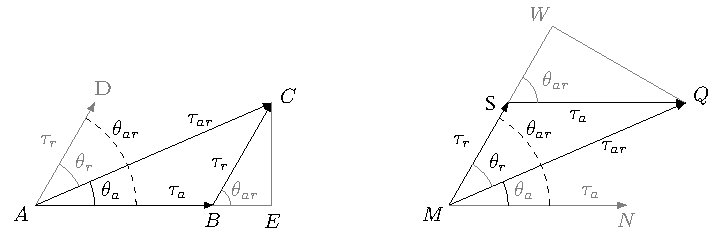
\includegraphics{figRotatingMachPrinciplesFluxAngles}
\begin{subfigure}{0.45\textwidth}
\centering
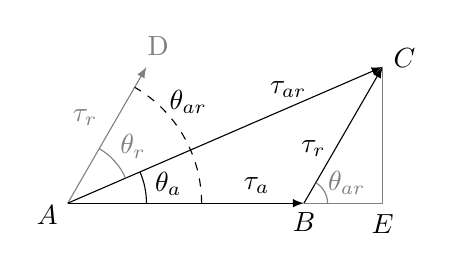
\begin{tikzpicture}
\draw[-latex](0,0)node[shift={(210:0.3cm)}]{$A$}--++(0:3 cm)coordinate(aTip)node[above,pos=0.8]{$\tau_a$}node[below]{$B$};
\draw[gray,-latex](0,0)--++(60:2 cm)node[above left,pos=0.5]{$\tau_r$}node[shift={(60:0.3 cm)}]{D};
\draw[-latex](aTip)--++(60:2cm)coordinate(rTip)node[left,pos=0.4]{$\tau_r$};
\draw[-latex](0,0)--(rTip)node[above,pos=0.7]{$\tau_{ar}$}node[shift={(23:0.3cm)}]{$C$}node[yshift=-2cm]{$E$};
\draw[gray](aTip)-|(rTip);
\draw[gray](aTip)++(0.3,0) arc (0:60:0.3 cm);
\draw[gray] (aTip)++(25:0.6 cm) node{$\theta_{ar}$};
%angles
\draw(0:1 cm) arc (0:23.413:1 cm);
\draw (11:1.3 cm) node{$\theta_{a}$};
%
\draw[gray](23.413:0.8 cm) arc (23.413:60:0.8 cm);
\draw[gray] (41:1.1 cm) node{$\theta_{r}$};
%
\draw[dashed](0:1.7 cm) arc (0:60:1.7cm);
\draw (40:2cm) node{$\theta_{ar}$};
\end{tikzpicture}
\caption{}
\end{subfigure}%
\begin{subfigure}{0.45\textwidth}
\centering
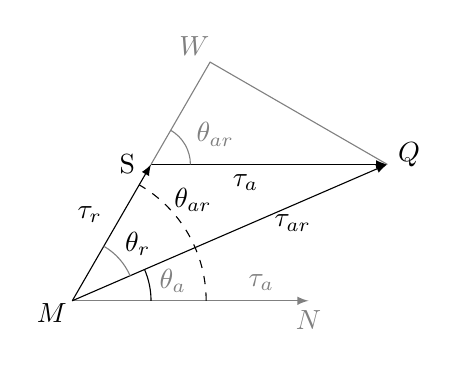
\begin{tikzpicture}
\draw[gray,-latex](0,0)node[black,shift={(210:0.3cm)}]{$M$}--++(0:3 cm)coordinate(aTip)node[gray,above,pos=0.8]{$\tau_a$}node[below]{$N$};
\draw[-latex](0,0)--++(60:2 cm)node[above left,pos=0.5]{$\tau_r$}coordinate(rTipR)node[shift={(180:0.3 cm)}]{S};
\draw[-latex](rTipR)--++(0:3 cm)coordinate(aTip)node[below,pos=0.4]{$\tau_a$};
\draw[-latex](0,0)--(aTip)node[below,pos=0.7]{$\tau_{ar}$}node[shift={(23:0.3cm)}]{$Q$};
\draw[gray](rTipR)--++(60:1.5 cm)node[shift={(-0.2,0.2)}]{$W$}--(aTip);
%angles
\draw(0:1 cm) arc (0:23.413:1 cm);
\draw (11:1.3 cm) node[gray]{$\theta_{a}$};
%
\draw[gray](23.413:0.8 cm) arc (23.413:60:0.8 cm);
\draw (41:1.1 cm) node{$\theta_{r}$};
%
\draw[dashed](0:1.7 cm) arc (0:60:1.7cm);
\draw (40:2cm) node{$\theta_{ar}$};
%
\draw[gray](rTipR)++(0.5,0) arc (0:60:0.5);
\draw[gray](rTipR)++(25:0.9)node{$\theta_{ar}$};
\end{tikzpicture}
\caption{}
\end{subfigure}%
\caption{مقناطیسی بہاو اور ان کے زاویے۔}
\label{شکل_گھومتے_مشین_بہاو_کے_زاویے}
\end{figure}
اسی طرح شکل \حوالہ{شکل_گھومتے_مشین_بہاو_کے_زاویے}-ب  کی تکون \عددیء{\Delta MWQ} اور تکون \عددیء{\Delta SWQ} میں \عددیء{WQ}  مشترک ہے جو درج ذیل ہو گا۔
\begin{align}
WQ=\tau_a \sin \theta_{ar}=\tau_{ar} \sin \theta_r
\end{align}
اس مساوات کی مدد سے مساوات \حوالہ{مساوات_گھومتے_مشین_مروڑ_بذریعہ_کوتوانائی_الف}  کو درج ذیل لکھا جا سکتا ہے۔
\begin{align}\label{مساوات_گھومتے_مشین_مروڑ_بذریعہ_کوتوانائی_پ}
T_m=-\frac{P}{2}\frac{\mu_0 \pi r l}{l_g} \tau_r \tau_{ar}  \sin \theta_r
\end{align}
مساوات \حوالہ{مساوات_گھومتے_مشین_مروڑ_بذریعہ_کوتوانائی_الف}،  مساوات \حوالہ{مساوات_گھومتے_مشین_مروڑ_بذریعہ_کوتوانائی_ب}  اور مساوات \حوالہ{مساوات_گھومتے_مشین_مروڑ_بذریعہ_کوتوانائی_پ}  کو ایک ساتھ لکھتے ہیں۔
\begin{gather}
\begin{aligned}\label{مساوات_گھومتے_مشین_مروڑ_بذریعہ_کوتوانائی_ت}
T_m&=-\frac{P}{2}\frac{\mu_0 \pi r l}{l_g} \tau_a \tau_r \sin \theta_{ar}\\
T_m&=-\frac{P}{2}\frac{\mu_0 \pi r l}{l_g} \tau_a \tau_{ar}  \sin \theta_a\\
T_m&=-\frac{P}{2}\frac{\mu_0 \pi r l}{l_g} \tau_r \tau_{ar}  \sin \theta_r
\end{aligned}
\end{gather}
ان مساوات سے  واضح ہے کہ میکانی قوت مروڑ کو دونوں لچھوں کے مقناطیسی دباو اور ان کے بیچ زاویہ کی صورت میں،  یا کسی ایک لچھے کے مقناطیسی دباو، کل مقناطیسی دباو اور ان کے بیچ زاویہ کی صورت میں لکھا جا سکتا ہے۔

اس بات کو یوں بیان کیا جا سکتا ہے کہ میکانی قوت مروڑ دو مقناطیسی دباو کی آپس میں ردعمل کی وجہ سے پیدا اور مقناطیسی دباو کی چوٹیوں اور ان کے بیچ زاویہ پر منحصر ہوتا ہے۔

مقناطیسی دباو، مقناطیسی شدت، کثافت مقناطیسی بہاو اور مقناطیسی بہاو  آپس میں تعلق رکھتے ہیں جنہیں مختلف طریقوں سے لکھا جا سکتا ہے۔ مثلاً خلائی درز میں کل مقناطیسی دباو \عددیء{\tau_{ar}} اور  درز میں  کثافت مقناطیسی بہاو \عددیء{B_{ar}} کا تعلق
\begin{align}
B_{ar}=\frac{\mu_0 \tau_{ar}}{l_g}
\end{align}
استعمال کر کے مساوات \حوالہ{مساوات_گھومتے_مشین_مروڑ_بذریعہ_کوتوانائی_ت}  کے آخری جزو کو درج ذیل لکھا جا سکتا ہے۔
\begin{align}\label{مساوات_گھومنے_مووڑ_بناوٹی_حدیں}
T_m=-\frac{P}{2} \pi r l \tau_r B_{ar} \sin \theta_r
\end{align}
مقناطیسی مشینوں کی  قالبی مقناطیسی مستقل \عددیء{\mu}  کی محدود قیمت کی بنا قالب میں کثافت مقناطیسی بہاو تقریباً ایک ٹسلا تک ہی بڑھائی جا سکتی ہے۔  مشین کی بناوٹ کے  وقت اس حد کو مد نظر رکھنا ہو گا۔ اسی طرح گھومتے لچھے کا مقناطیسی دباو اس لچھے میں برقی رو پر منحصر ہوتا ہے۔ اس برقی رو سے لچھے کی مزاحمت میں برقی توانائی ضائع ہوتی ہے جس سے لچھا گرم ہوتا ہے۔ برقی رو کو اس حد تک بڑھایا جا سکتا ہے جہاں تک لچھے کو ٹھنڈا رکھنا ممکن ہو۔ یوں مقناطیسی دباو کو ایک حد  سے نیچے رکھنا ہو گا۔ مساوات \حوالہ{مساوات_گھومنے_مووڑ_بناوٹی_حدیں} میں  \عددی{B_{ar}} اور \عددی{\tau_r} دونوں صریحاً موجود ہیں لہٰذا مشین کی بناوٹ کے نقطہ نظر سے یہ ایک اہم مساوات ہے۔ 

 مساوات \حوالہ{مساوات_گھومنے_مووڑ_بناوٹی_حدیں} کی دوسری اہم صورت دیکھتے ہیں۔  قطب پر اوسط کثافت مقناطیسی بہاو \عددیء{B_{\textup{اوسط}}} اور قطب کے رقبہ  \عددیء{A_P}
\begin{align}
B_{\textup{اوسط}}&=\frac{1}{\pi} \int_{-\frac{\pi}{2}}^{+\frac{\pi}{2}} B_0 \cos \theta \dif \theta=\frac{2 B_0}{\pi}\\
A_P&=\frac{2\pi rl}{P}
\end{align}
 کا حاصل ضرب قطب پر مقناطیسی بہاو \عددیء{\phi_P} ہوتا ہے لہٰذا
\begin{align}
\phi_P=\frac{2 B_0}{\pi}\frac{2\pi rl}{P}
\end{align}
اور
\begin{align}\label{مساوات_گھومتے_مشین_مروڑ_اور_بہاو}
T_m=-\frac{\pi}{2} \left(\frac{P}{2} \right)^2 \phi_{ar} \tau_r \sin \theta_r
\end{align}
ہوں گے۔ مساوات \حوالہ{مساوات_گھومتے_مشین_مروڑ_اور_بہاو} معاصر مشینوں  کے لئے بہت کار آمد ہے۔
